\singlespacing
\chapter{Bilan de C de la tourbière de La Guette}
\label{ch:ch3}

\minitoc

\newpage
\doublespacing
\section{Introduction}
Les tourbières jouent un rôle important de stockage du carbone à l'échelle globale (cf chapitre~\ref{ch:ch1}).
En outre, ces écosystèmes ont une diversité importante que ce soit dans leur fonctionnement naturel ou les perturbations qu'elles subissent.
Cependant il existe peu d'estimations de leur bilan de carbone prenant en compte à la fois la contribution du \coo, du \chh et du COD.
La majorité des écosystèmes tourbeux pour lesquels un bilan de carbone a été estimé se situe sous les hautes latitudes de l'hémisphère nord comme en Suède \citep{waddington2000,peichl2014}, en Finlande \citep{Alm1997}, au Canada \citep{trudeau2014}.
Les estimations du bilan de carbone de tourbières situées plus au sud, notamment en Europe, sont plus rares (exemple d'une tourbière du Jura français, \citealp{bortoluzzi2006a}). 
De nombreuses études ont été faites sur les tourbières au Canada, mais le climat y est différent, avec des hivers plus froids pour des latitudes équivalentes.
L'étude de ces écosystèmes présents à la limite sud de leur extension est importante.
En effet, ils expérimentent des conditions plus extrêmes que les autres et qui, sans être identiques, peuvent se rapprocher de celles que subiront certains écosystèmes tourbeux suite au réchauffement climatique.

Plus spécifiquement, le site d'étude, la tourbière de La Guette, est représentative d'une grande partie des tourbières vis-à-vis des perturbations qu'elle subit : drainage et envahissement par une végétation vasculaire (les caractéristiques du site sont détaillées dans le chapitre~\ref{ch:ch2}).
On s'attend à ce que cet envahissement se traduise par une aération du milieu plus importante, liée au développement des racines.
Cette aération favoriserait une RE élevée et un fonctionnement en source de carbone.

Le \textbf{premier objectif} de ce chapitre est donc d'\textbf{établir le bilan de C} de la tourbière de La Guette, afin de mieux comprendre comment fonctionne cet écosystème et de mettre en perspective ce fonctionnement par rapport aux tourbières des hautes latitudes.

Le \textbf{second objectif} est de \textbf{caractériser la variabilité spatiale} de ces flux de GES à travers ce bilan de C.
En effet les tourbières sont des écosystèmes avec des conditions environnementales qui peuvent varier dans l'espace.
Par exemple le niveau de la nappe d'eau peut, à cause de variation micro-topographique, être plus ou moins élevé, immerger la surface du sol avec des zones d'eau libre ou au contraire être quelques dizaines de centimètres sous la surface du sol.
La conséquence de ces variations est l'existence de micro-environnements différents qui abritent des communautés végétales et microbiennes différentes.
Finalement les variations des conditions environnementales contrôlant les flux, entraînent la variation des flux.
Estimer ces variations est donc nécessaire afin de préciser dans quelle mesure elles influent sur le bilan de C.

\section{Procédure expérimentale et analytique}

Cette partie contient la description de la stratégie d'échantillonnage et le détail des méthodes de mesure, les méthodes de chambres utilisées pour la mesure de flux de GES ont été détaillées dans la partie~\ref{sec:clsd_chbr_method}.
Elle explicite également le calcul de variables élaborées utilisées par la suite, détaille le principe permettant l'estimation du bilan de carbone du site à l'échelle saisonnière et décrit la stratégie d'étude de la variabilité spatiale.
Enfin elle précise comment sont calculées les erreurs associées aux flux et bilans.

\subsection{Protocole d'observation}

En juin 2011, 20 placettes ont été installées selon un échantillonnage aléatoire stratifié:
La surface de la tourbière active (\SI{13}{\hectare}) a été divisée selon une grille de 20 mailles et un point, choisi aléatoirement dans chaque maille, localise chaque placette (Figure~\ref{fig:carteVS}).
La taille de la maille a été ajustée de manière à avoir vingt carrés sur la surface de la tourbière.
Cette méthode permet de conserver un échantillonnage aléatoire tout en ayant une représentativité spatiale homogène du site. 
Les placettes, délimitées par des piquets, occupent une surface de \SI{4}{\square\metre} (2$\times$\SI{2}{\metre}).
Usuellement, les placettes sont séparées en groupes micro-topographiques (Figure~\ref{fig:microtopo}), avec des embases positionnées sur les buttes (\textit{hummock}), les trous (\textit{hollows}) et les zones d'eau libre (\textit{pool}) \citep{Alm1997,waddington2000}.
Ou encore selon différents traitements, réhabilité/non réhabilité, exploité/non exploité, manipulé/non manipulé \citep{bortoluzzi2006a,strack2013}.
Cette méthodologie présente l'avantage de permettre une distinction fine des capacités sources/puits entre ces traitements.
Cependant elle implique généralement un placement des embases proches les unes des autres au sein d'un même traitement, limitant la représentativité spatiale des mesures.
Le placement des 20 embases sur l'ensemble du site, sa taille l'autorisant, permet de gagner en représentativité spatiale.
Sur ces placettes ont été réalisées des mesures de \textbf{flux de gaz} et de \textbf{variables environnementales}.

\begin{figure}
\centering
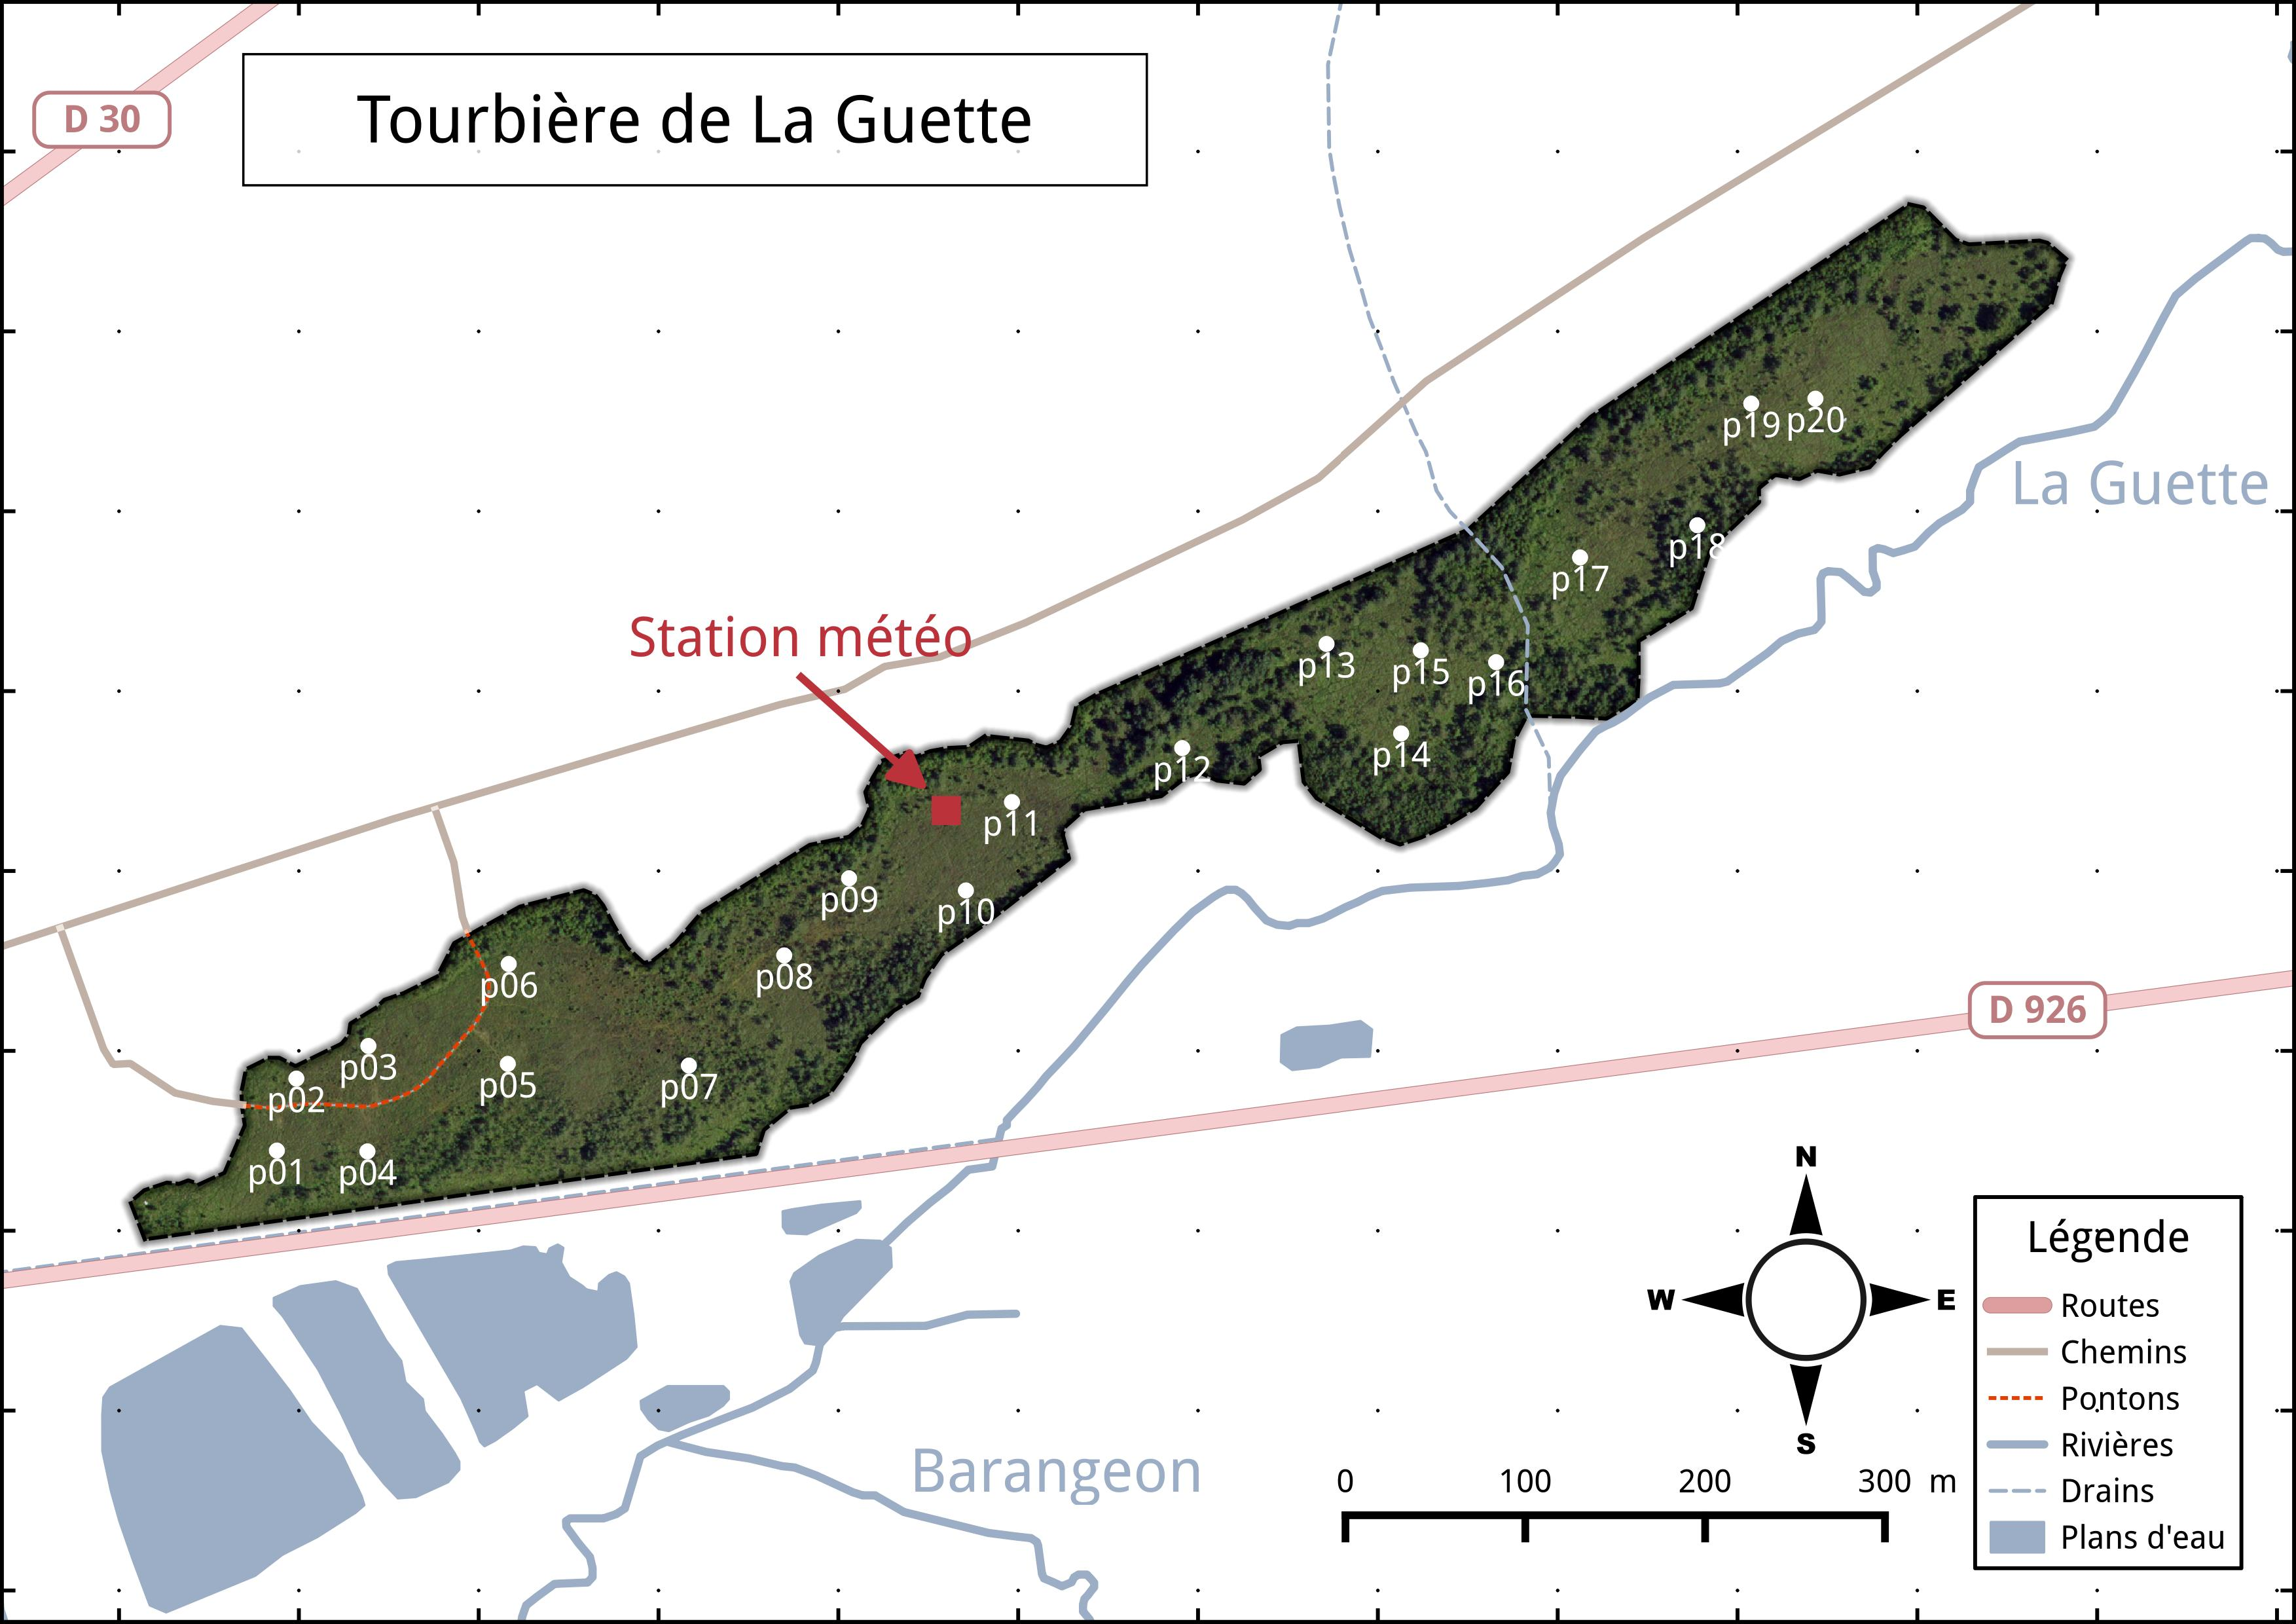
\includegraphics[width=\textwidth]{chap3/carteVS}
\caption{Répartition des 20 placettes de mesures suivant un échantillonnage aléatoire stratifié.}
\label{fig:carteVS}
\end{figure}

\subsubsection{Mesures des flux de gaz}

Les mesures des flux de \coo et de \chh ont été effectuées en utilisant les méthodes de chambres décrites dans la partie~\ref{sec:clsd_chbr_method}.
À l'intérieur de chaque placette ont été installés de façon permanente un piézomètre et une embase permettant la mesure des flux de gaz (les embases sont décrites dans le chapitre~\ref{ch:ch2}, partie~\ref{subsec:ss_mes_co2}).

Initialement, les flux de \coo, \chh et N\textsubscript{2}O devaient être mesurés et étudiés (Tableau~\ref{table:ls_var}).
Cependant, suite à des tests préliminaires effectués sur la tourbière montrant des émissions très faibles de N$_{2}$O, ce gaz n'a pas été étudié.
Les mesures de \coo ont été effectuées de mars 2013 à février 2015, avec une fréquence quasiment mensuelle (20 campagnes, pour 24 mois de mesures, sur les 20 placettes). 
Chaque campagne de mesures s'étend sur deux journées et nécessite la présence de deux personnes afin de pouvoir mesurer l'ensemble des 20 placettes.
Les mesures de \chh ont été effectuées avec une fréquence et sur un nombre d'embases inférieurs (12 campagnes, 5 embases).
Ceci a été déterminé par la difficulté de déploiement \textit{in-situ} de l'instrument SPIRIT : il est lourd, difficilement transportable dans un milieu tourbeux et nécessite entre chaque déplacement un temps de mise en marche/arrêt important (plus de \SI{30}{\minute}).
Les mesures se sont donc limitées aux placettes accessibles depuis le ponton (placette n°1 à 6, figure~\ref{fig:carteVS}).

\subsubsection{Mesures du COD}

Des échantillons d'eau ont été prélevés à l'exutoire de la tourbière, et leur concentration en COD a été mesurée moins de 24 heures après le prélèvement.
Les analyses de COD ont été faites, après filtration à \SI{0.45}{\micro\metre}, en utilisant la technique dite NPOC (\textit{Non Purgeable Organic Carbon}) dans laquelle le carbone inorganique présent dans l'échantillon est transformé en \coo par l'ajout d'un acide puis évacué (purgé) avant que l'échantillon ne soit injecté dans un four et analysé par un détecteur Infra-rouge.

\subsubsection{Mesures des variables environnementales}


\begin{table}
\centering
\caption{Liste des variables acquises. Les données acquises manuellement sont réalisées sur les 20 placettes, tandis que les données acquises automatiquement sont réalisées par la station météorologique (1 seul point).}
\label{table:ls_var}
\begin{tabular}{llll}
\toprule
& variable & type d'acquisition & fréquence \\
\midrule
\multicolumn{4}{l}{Flux} \\ [+.5ex]
& \coo & manuelle & mensuelle \\
& \chh & manuelle & mensuelle \\[+1ex]
\multicolumn{4}{l}{Physique} \\ [+.5ex]
& rayonnement photosynthétique actif & manuelle & mensuelle \\
& température air & manuelle & mensuelle \\
& température sol & manuelle & mensuelle \\
& température air & automatique & horaire \\
& température sol & automatique & horaire \\[+1ex]
\multicolumn{4}{l}{Hydrologie} \\ [+.5ex]
& niveau de nappe & manuelle & mensuelle \\
& niveau de nappe & automatique & horaire \\
& conductivité & manuelle & mensuelle \\
& pH & manuelle & mensuelle \\
& COD & manuelle & mensuelle \\
& teneur en eau & manuelle & mensuelle \\[+1ex]
\multicolumn{4}{l}{Végétation} \\ [+.5ex]
& pourcentage de recouvrement végétal & manuelle & mensuelle \\[+1ex]
\multicolumn{4}{l}{Météorologie} \\ [+.5ex]
& pluviométrie & automatique & horaire \\
& pression atmosphérique & automatique & horaire \\
& humidité de l'air & automatique & horaire \\
& rayonnement solaire & automatique & horaire \\
& vent (vitesse et direction) & automatique & horaire \\
\bottomrule
\end{tabular}
\end{table}


Les variables environnementales mesurés manuellement sont la pression atmosphérique, le rayonnement photosynthétique actif (\textit{photosyntheticaly active radiation}, PAR), les températures du sol à différentes profondeurs, la végétation (pourcentage de recouvrement), le niveau de la nappe d'eau (Tableau~\ref{table:ls_var}).
La pression atmosphérique est mesurée au début et à la fin des mesures de flux.
Le PAR est mesuré au début et à la fin des mesures de l'ENE.
Le recouvrement de végétation est estimé visuellement.
Des prélèvements d'eau ont été effectués chaque mois pour mesurer le pH et la conductivité (mesures effectuées sur le terrain après les mesures de flux).
Les échantillons d'eau prélevés dans les 20 placettes ont été congelés pour la mesure ultérieure de la concentration en carbone organique dissout (COD).
Dans les tourbières la quantité de carbone inorganique est généralement considérée comme négligeable \citep{worrall2009}.

L'ensemble de ces mesures nécessitant d'accéder aux placettes régulièrement, des planches de bois ont été utilisées comme pontons mobiles pour limiter les perturbations. La dispersion des placettes sur l'ensemble du site a rendu impossible une installation plus permanente.

Les mesures automatiquement acquises via la station météo installée sur le site depuis 2010 sont la température de l'air, la température de la tourbe à \num{-5}, \num{-10}, \num{-20} et \SI{-40}{\centi\metre} de profondeur, la vitesse et la direction du vent, l'humidité relative de l'air, le rayonnement solaire, et la pression atmosphérique (Tableau~\ref{table:ls_var}).

\subsection{Variables élaborées utilisées}

Les mesures de recouvrement de la végétation ont été sommées par strate végétale.
On utilisera donc RSM, RSH, RSA pour distinguer respectivement les recouvrements de la strate muscinale (\textit{Sphagnum spp.}), herbacée (\textit{Molinia caerula} et \textit{Eriophorum augustifolium}) et arbustive (\textit{Erica tetralix} et \textit{Calluna vulgaris}).
Un indice de végétation, représentant la quantité de végétation présente dans une embase est également calculé de la façon suivante : 

\begin{equation}
IV = \frac{RSM + RSA + RSH}{\sum R{max}}
\end{equation}

Avec :
\begin{itemize}
\item $\sum R_{max}$ La somme des pourcentages de recouvrement maximum par strates.
\item RSM le pourcentage de recouvrement de la strate muscinale mesuré
\item RSH le pourcentage de recouvrement de la strate herbacée mesuré
\item RSA le pourcentage de recouvrement de la strate arbustive mesuré
\end{itemize}

Le niveau de nappe est composé de deux mesures, l'une du haut du piézomètre jusqu'au niveau de la nappe et l'autre du haut du pièzomètre jusqu'à la surface du sol. 
Par la suite, et en l'absence de précisions, le niveau de nappe se réfère à la différence entre ces deux mesures et donc à la distance entre la surface du sol et le niveau de la nappe (négative sous la surface du sol et inversement).
En cas de présence de Sphaignes, le haut des capitulums est pris comme référence (z=0).

\subsection{Estimation des flux de GES dans le bilan de C}

L'estimation des flux de GES pour calculer un bilan de carbone se fait en trois étapes.
La première consiste à établir des relations empiriques entre les flux et un ou plusieurs variables environnementales.
C'est la phase de \textbf{calibration}.
La seconde, l'\textbf{évaluation}, teste la pertinence de ces relations sur un jeu de données indépendantes.
La troisième, l'\textbf{interpolation}, utilise ces relations empiriques et les données acquises à plus haute fréquence, pour intégrer dans le temps les mesures ponctuelles sur l'ensemble des deux années de mesure. 
La chronique ainsi reconstituée permet ensuite d'estimer les quantités de carbone annuelles déplacées via les différents flux et d'en calculer leur bilan.

\subsubsection{Calibration}

Pour estimer le bilan de carbone du site il est donc nécessaire d'établir des modèles reliant des flux mesurés ponctuellement avec des variables explicatives mesurées à haute fréquence (par exemple entre la respiration de l'écosystème et la température de l'air).
Pour établir ces modèles empiriques, les données acquises ont été moyennées par campagne de mesures ; ceci permettant, dans un premier temps, de s'affranchir de la variabilité spatiale des flux et ne considérer que la variabilité temporelle.
Les relations entre flux et variables environnementales ont ensuite été étudiées deux à deux, notamment en réalisant une analyse en composante principale (ACP).
Cette analyse permet de déterminer quelles sont les relations entre les variables et plus particulièrement quelles sont celles qui déterminent le plus les flux de GES.
Le nombre de données acquises pour le \coo et le \chh étant différent, une ACP a été réalisée pour chacun de ces gaz (Annexe~\ref{sec:acp}).
Une fois le facteur de contrôle prépondérant d'un gaz établi, grâce à l'ACP et à la littérature, une relation empirique est établie entre les deux.
Elles sont évaluées à l'aide du coefficient de détermination ajusté (R\textsuperscript{2}) et de la racine carré de l'erreur quadratique normalisée par la moyenne (\textit{Normalised Root Mean Square Error}, NRMSE).
Le R$^{2}$ est utilisé comme indicateur de la proportion de la variabilité des données expliquée par le modèle, sa valeur est comprise entre 0 et 1 (pour les équations linéaires) : 

$$ R^{2}_{non~ajust\acute{e}} = 1 - \frac{\sum(y-\hat{y})^2}{\sum(y-\bar{y})^2} $$ 

Avec : 
\begin{itemize}
\item $R^{2}_{non~ajust\acute{e}}$ : le R\textsuperscript{2} non ajusté
\item $y$ : données mesurées
\item $\hat{y}$ : données modélisées
\item $\bar{y}$ : la moyenne des données mesurées
\end{itemize}

$$ R^{2} = 1 - (1-R^{2}_{non~ajust\acute{e}})\frac{n-1}{n-p-1} $$ 

Avec : 
\begin{itemize}
\item $R^{2}$ : le R\textsuperscript{2} ajusté
\item $R^{2}_{non~ajust\acute{e}}$ : le R\textsuperscript{2} non ajusté
\item $n$ : le nombre d'observations
\item $p$ : nombre de variables explicatives
\end{itemize}

La RMSE et sa normalisation par la moyenne NRMSE sont utilisées comme indicateur de l'écart entre les données mesurées et les données modélisées :

$$ RMSE = \sqrt{\frac{\sum(y - \hat{y})^2}{n}} $$

$$ NRMSE = 100 \times \frac{RMSE}{\bar{y}} $$

Avec les notations précédentes et : 
\begin{itemize}
\item $n$ : le nombre d'observations
\end{itemize}
Les résidus\footnote{Les résidus sont définit comme la différence entre les valeurs mesurées et celles calculées par un modèle.} sont également étudiés dans le but d'éviter un biais ou une hétéroscédasticité\footnote{On parle d'homoscédasticité lorsque la variance de l'erreur d'une variable est constante, et l'hétéroscédasticité lorsque qu'elle ne l'est pas} dans les données (Figure~\ref{fig:ref_resid}).

\begin{figure}[!htb]
\centering
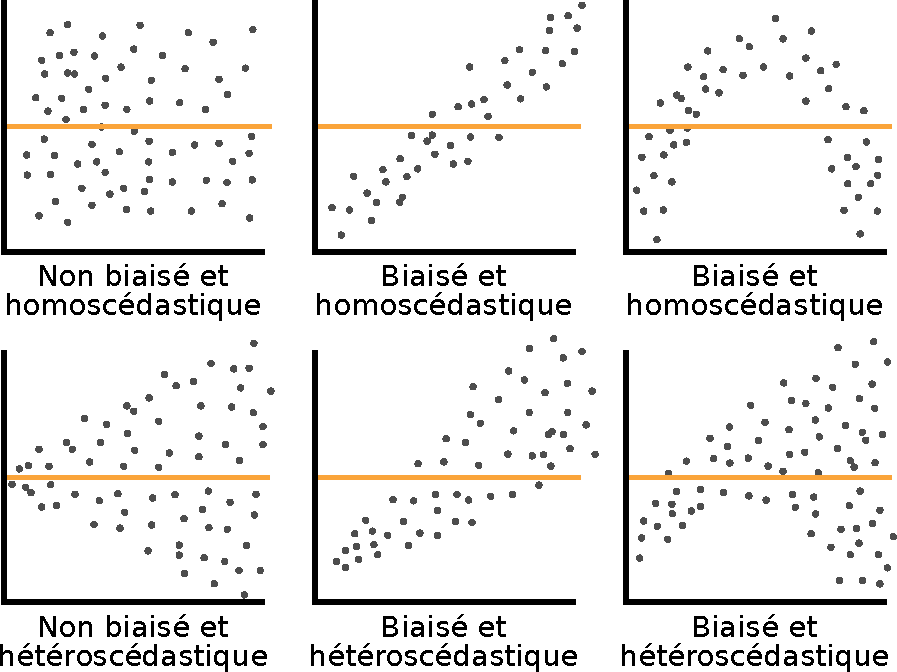
\includegraphics[width=\textwidth]{chap3/ref_resid}
\caption{Cas idéaux de distribution des résidus. Modifié d'après source inconnue, repris de : \url{https://danieljhocking.wordpress.com/2011/07/18/model-validation-interpreting-residual-plots/}}
\label{fig:ref_resid}
\end{figure}

Puis les résidus de ces modèles de base ont été étudiés en fonction des variables environnementales restantes.
Dans le cas où une tendance est visible avec l'un d'entre eux, le facteur est ajouté \citep{bortoluzzi2006a}.
En plus des indicateurs précédents, la pertinence de l'ajout d'un paramètre est évalué à l'aide du  critère d'information d'Akaike (\textit{Akaike Information Criterion}, AIC) \citep{akaike1974,burnham2002} :

$$ AIC = -2 \times log(L) + 2\times k $$ 

Avec :
\begin{itemize}
\item $L$ : le maximum de la fonction de vraisemblance
\item $k$ : le nombre de paramètres à estimer
\item $\bar{y}$ : la moyenne des données mesurées
\end{itemize}

L'AIC est un indicateur qui permet de déterminer si l'ajout d'un paramètre dans un modèle est pertinent (autrement dit, si l'ajout d'un paramètre vaut l'information qu'il apporte), afin d'éviter de le sur-ajuster.
Pour cela on considère la valeur la plus faible de l'AIC comme le meilleur indicateur.

La température a été choisie comme base de départ à la construction des modèles de RE et PPB, car (i) c'est le facteur de contrôle le plus souvent invoqué dans la littérature et (ii) les corrélations avec les flux étaient les plus fortes (cf ACP, annexe~\ref{sec:acp}).

\begin{center}
\begin{minipage}{.85\textwidth}
\setlength{\parindent}{-10pt}%
\onehalfspacing
\textbf{Remarque :} La RE, et l'ENE sont des flux mesurés directement sur le terrain à l'inverse de la PPB.
Cette dernière est déduite des deux flux précédents en utilisant l'équation $PPB = ENE - RE$.
Elle sera néanmoins appelée PPB mesurée, par opposition aux flux modélisés.
Afin d'établir le bilan de carbone tout en gardant une discrimination entre les flux entrants et sortants de l'écosystème la RE et la PPB ont été estimés séparément.
\end{minipage}
\end{center}

Concernant la respiration de l'écosystème, les températures utilisées dans la littérature sont variables.
La température la plus utilisée est la température du sol à \SI{-5}{\centi\metre}  \citep{ballantyne2014}.
D'autres auteurs utilisent aussi la température de l'air et la température du sol à \SI{-10}{\centi\metre} \citep{bortoluzzi2006a,kim1992}.
L'utilisation de ces profondeurs est justifiée par le fait que dans la tourbe, la respiration du sol est la plus importante au dessus du niveau de l'eau et donc en surface \citep{Luo200661}.
C'est également en surface que se situent la majorité des racines \citep{rydin2013c}.
La respiration des racines contribue à la respiration de l'écosystème pour 35 à \SI{60}{\percent} \citep{silvola1996,crow2005}.

Il ne semble pas émerger de consensus dans la littérature quant aux facteurs contrôlant les émissions de \chh.
Différents facteurs sont utilisés comme la température \citep{alm1999,bubier1995b}, le niveau de la nappe \citep{bubier1993a} ou encore la végétation \citep{bortoluzzi2006a}.
Ces facteurs peuvent être utilisés seuls ou conjointement.

\subsubsection{Évaluation}

Après la phase de calibration, les facteurs de contrôle utilisés dans les modèles ont été évalués à l'aide de données indépendantes acquises en 2014, dans le cadre d'un suivi expérimental mis en place sur la tourbière de La Guette pour le projet CARBIODIV (cf annexe~\ref{sec:carbiodiv}).
Les méthodes de mesures des flux de \coo et de \chh sont strictement identiques (ainsi que les opérateurs) à celles utilisées pour établir le bilan de carbone.
En revanche le positionnement des placettes est beaucoup plus classique : proches les unes des autres, et avec différents traitements.
Afin de pouvoir les comparer, seules les placettes de contrôles, (n'ayant donc subi aucune manipulation) de cette expérimentation seront utilisées, soit 4 placettes dans une station en amont et 4 en aval de la tourbière de La Guette.
Le terme d'évaluation est ici préféré à celui de validation car le nouveau jeu de données utilisé, bien qu'indépendant de celui utilisé pour la calibration, n'a pas été acquis de manière strictement identique, notamment au niveau de la représentativité spatiale (répartition des embases sur le site).

\subsubsection{Interpolation}

Enfin les variables environnementales ont été interpolés à une fréquence horaire identique à celle de la station météo présente sur le site:
pour des données dont l'acquisition est manuelle uniquement, comme la végétation, une interpolation linéaire est faite entre les points de mesures.
Pour les données acquises à la fois automatiquement par la station météorologique et manuellement, comme la température de l'air ou de la tourbe, l'interpolation est faite à partir de la relation entre les mesures continues et ponctuelles.
Les flux sont ensuite recalculés (en \si{\micro\mole\per\square\meter\per\hour}) à l'échelle horaire sur les deux années de mesure puis sommés afin d'estimer les bilans de carbone.
Ces bilans sont par la suite exprimés en \si{\gram C m^{-2}} par période de temps à l'année, sauf quand précisé.

Le détail des équations utilisées et de la qualité des différents modèles est présenté dans la partie résultats.

\subsection{Estimation des flux de carbone organique dissout dans le bilan de C}

En plus des flux gazeux, les flux de COD sont pris en compte dans le bilan de carbone.
Le flux de COD entrant dans la tourbière est estimé à partir des précipitations et de leur concentration en COD.
La concentration en COD des eaux de pluie est généralement comprise entre \num{0.5} et \SI{2.5}{\milli\gram\per\litre}\citep{sigg2014}.
Le flux de COD sortant est calculé à partir des résultats  du modèle de \citet{binet2013} permettant d'estimer une quantité d'eau sortant à l'exutoire du bassin versant de l'écosystème et des concentrations en COD mesurées pendant les deux années de mesure.

\begin{equation}
\label{eq:COD}
F_{COD} = \overbrace{(P\times[COD]_{P})}^{C entrant}-\overbrace{(D\times[COD]_{E})}^{C sortant}
\end{equation}

Avec :
\begin{itemize}
\item $F_{COD}$ : le flux de COD
\item $P$ : les précipitations en \si{\litre\per\square\metre}
\item $[COD]_{P}$ : la concentration en COD des précipitations (fixé à \SI{1}{\mgl})
\item $D$ : la décharge en eau du système à l'exutoire (quantité d'eau qui sort du bassin versant en \si{\litre})
\item $[COD]_{E}$ : la concentration en COD de l'eau à l'exutoire 
\end{itemize}

\subsection{Variabilité spatiale des flux et du bilan de carbone}

La variabilité spatiale des flux a été caractérisée en utilisant deux approches.
La première consiste à calibrer par placette les modèles sélectionnés lors de la modélisation à l'échelle de l'écosystème.
Cette opération permet ainsi de calculer des flux par placette.
L'inconvénient de cette méthode est le faible nombre de points utilisés pour chaque calibration, ce qui peut conduire à une erreur importante sur l'estimation des paramètres voire à la non convergence des modèles.
La seconde approche permet de pallier en partie ce problème en calibrant les modèles à partir de groupes de placettes.
Ces ensembles ont été faits en regroupant les placettes ayant la composition végétale la plus proche.
Ce choix se justifie par le fait que la végétation joue un rôle important sur les flux de carbone (photosynthèse, transport).
La température, plus facile à mesurer, et le niveau de la nappe, qui n'a que peu varié, semblaient des choix moins pertinents. 
Le partitionnement à été fait par classification hiérarchique ascendante.
C'est une méthode déterministe qui consiste, à partir de l'ensemble des individus (ici nos différentes placettes de mesure), à les regrouper en classes de plus en plus grandes.
Les points sont regroupés par similarité, les deux points les plus proches sont fusionnés, puis les deux suivants et ce jusqu'à ce qu'il ne reste qu'une seule classe.
Cette classification est généralement représentée par un dendrogramme.
Elle a été appliquée sur les recouvrements végétaux mesurés et permet de distinguer quatre groupes (Figure~\ref{fig:tree}).
Le nom de ces groupes (Chaméphyte ligneux, Graminoïde, Hétérogène et Bryophytes) reflète la végétation majoritaire.

\begin{figure}[t]
\centering
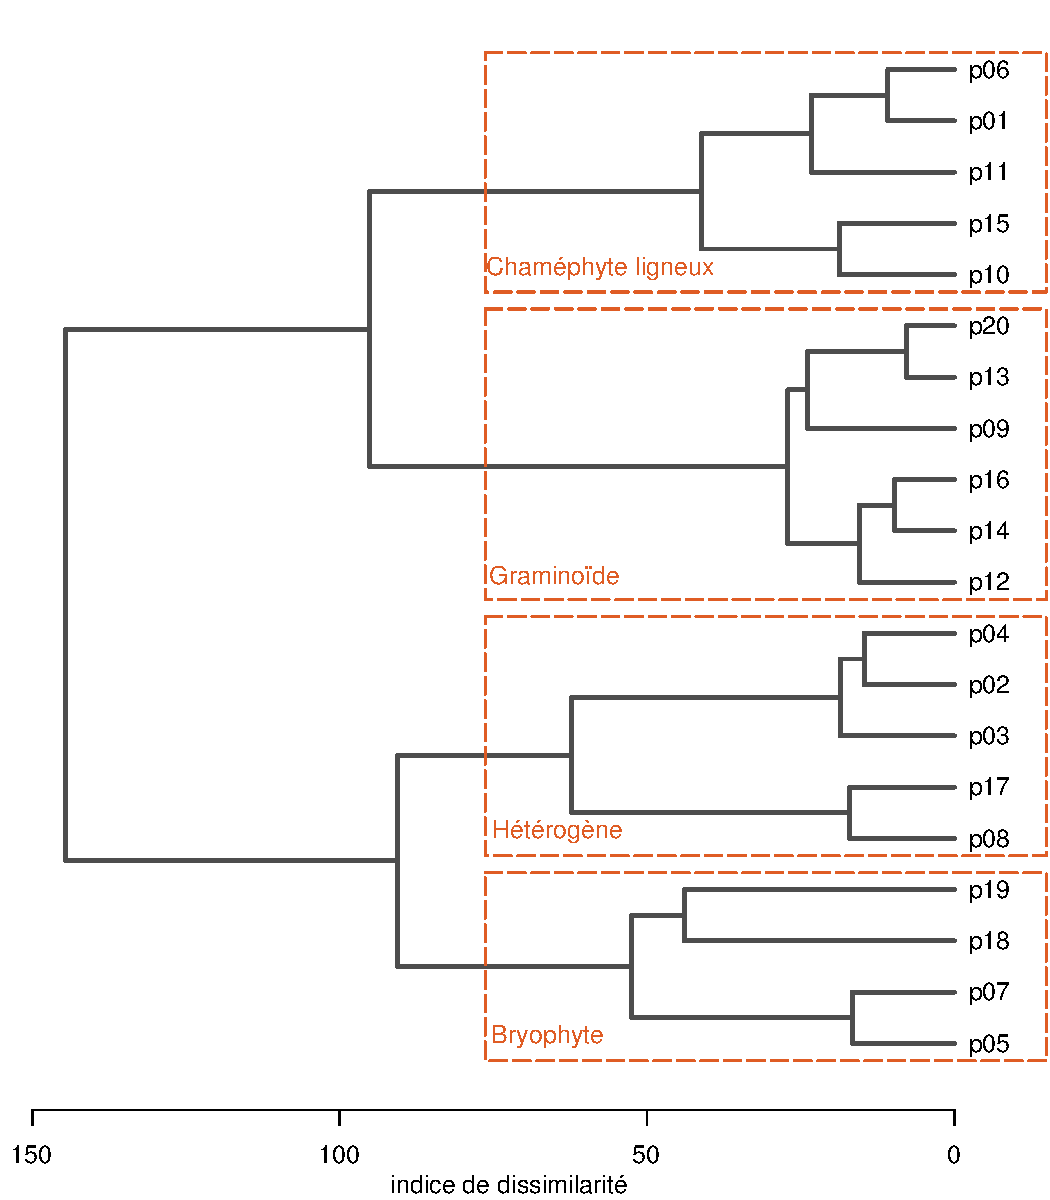
\includegraphics[width=.8\textwidth]{chap3/tree}
\caption{Partitionnement des placettes en fonction de leur similarité en termes de composition végétale (pourcentage des strates muscinales, herbacées et arbustives). L'algorithme Lance-Williams est utilisé avec une matrice de distance euclidienne.}
\label{fig:tree}
\end{figure}


\subsection{Estimation de l'erreur associée aux flux et aux bilans}
\label{subsec:erreur_bilan}

Pour chaque flux, l'erreur sur le bilan annuel est calculé en multipliant ce flux par l'erreur quadratique normalisée, calculée lors de la calibration.
Pour les bilans, l'erreur associée est calculée comme la somme des erreurs associées aux flux composant le bilan.
Chacune de ces erreurs est pondérée en fonction de leur importance relative par rapport à la somme des flux en valeur absolue \citep{waddington2000}.

\begin{equation}
E_{(bilan)} = (\chi_{PPB} \times NRMSE_{PPB}) + (\chi_{RE} \times NRMSE_{RE}) + (\chi_{\fchh} \times NRMSE_{\fchh})
\end{equation}

Avec : 
\begin{itemize}
\item $E_{(bilan)}$ l'erreur associée au bilan
\item $\chi_{flux}$ la fraction du flux par rapport à la somme en valeur absolue de tous les flux compris dans le bilan
\item $NRMSE_{flux}$ la racine carrée de l'erreur quadratique normalisée à la moyenne associée au flux
\end{itemize}

Ces erreurs ne sont qu'une part de l'erreur totale qui devrait être associée à ces flux. Elle ne considère pas les erreurs aléatoires et systématiques liées aux mesures, qui sont supposées négligeables par rapport à l'erreur provenant de l'estimation des paramètres des équations et de la variablité spatiale des flux.


\section{Résultats}

\subsection{Cinétique des variables environnementales et des flux de GES}

\subsubsection{Variables environnementales}

\begin{figure}
\centering
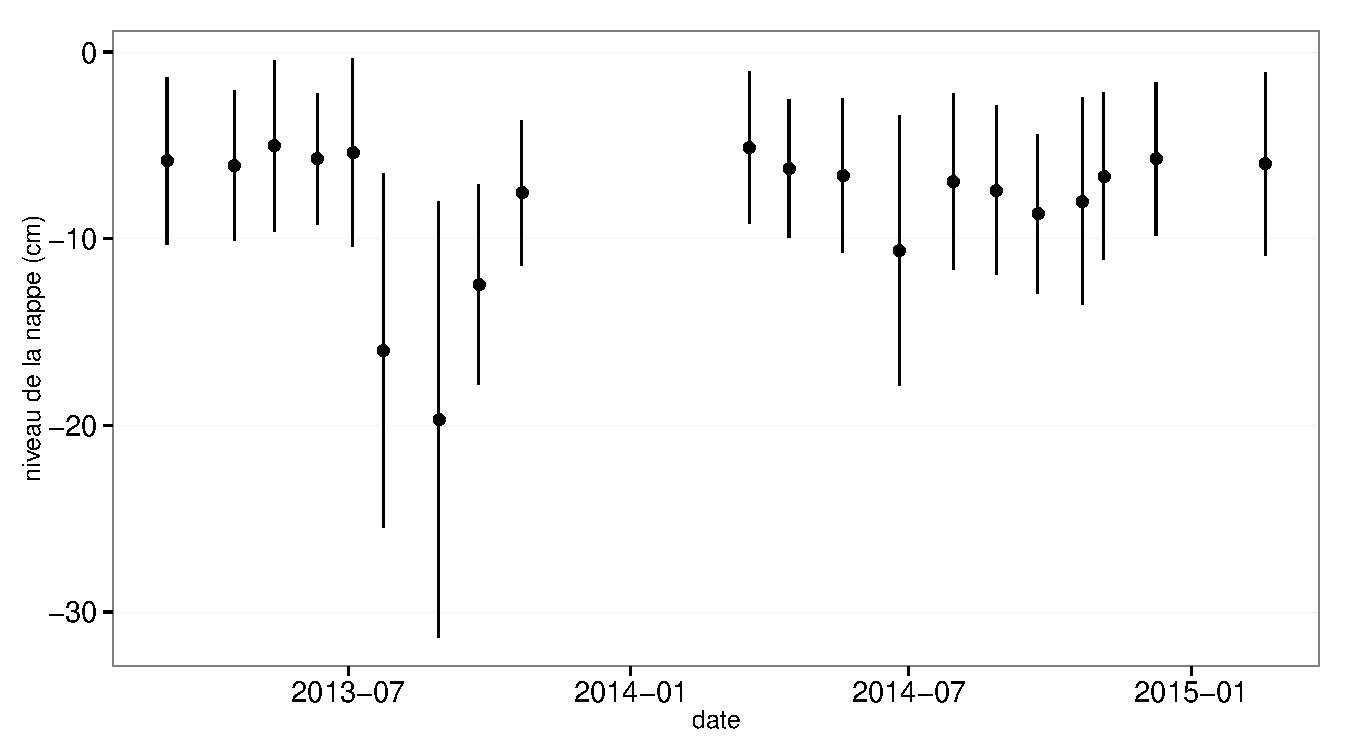
\includegraphics[width=1.15\textwidth, center]{chap3/WTL_mean_evolution}
\caption{Variabilité temporelle du niveau moyen de la nappe mesuré dans les 20 placettes entre mars 2013 et février 2015. Les valeurs correspondent à la distance entre le niveau de nappe et la surface du sol (en cm).}
\label{fig:WTL_mean_evolution}
\end{figure}

L'évolution du niveau de la nappe d'eau mesuré manuellement dans les 20 placettes est marquée par un étiage d'une vingtaine de centimètres en moyenne en 2013 et l'absence d'un étiage net en 2014 (Figure~\ref{fig:WTL_mean_evolution}).
Le niveau de la nappe moyen ne descend pas en dessous de \SI{-10}{\cm} avec \num{-9.2(76)} et \SI{-7.1(48)}{\centi\metre} respectivement pour 2013 et 2014.
Ces observations sont cohérentes avec les mesures acquises automatiquement et à plus haute fréquence (Figure~\ref{fig:WTL}) et confirment l'étiage particulièrement important de ces deux années par rapport aux précédentes.

\begin{figure}
\centering
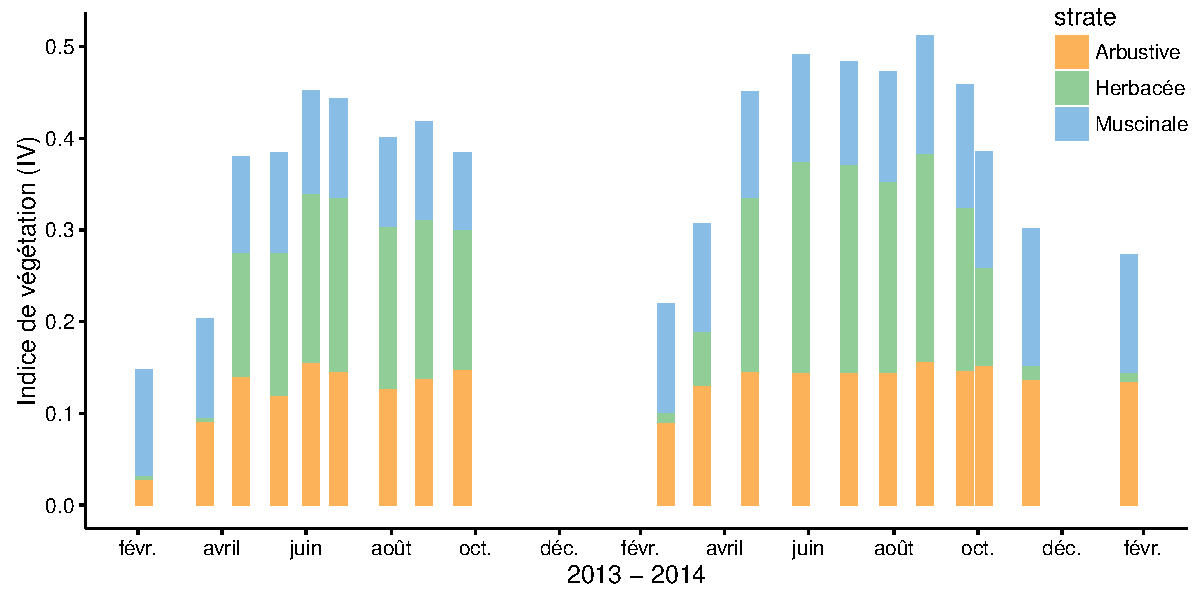
\includegraphics[width=1\textwidth, center]{chap3/veg_evol}
\caption{Variabilité de la valeur et de la composition (proportion des différentes strates végétales) de l'indice de végétation (IV) au cours du temps entre mars 2013 et février 2015, 
Évolution de la végétation à travers l'indice de végétation et des strates qui le composent}
\label{fig:veg_evol}
\end{figure}

L'évolution saisonnière de la végétation sur la tourbière de La Guette est visible (Figure~\ref{fig:veg_evol}).
Cette variabilité est majoritairement contrôlée par la strate herbacée qui hiverne à la fin de la saison de végétation, perdant ses parties aériennes, à l'inverse des chaméphytes ligneux et des bryophytes.
La saison de végétation, pour les herbacées, a commencé un peu plus tôt en 2014 (Figure~\ref{fig:veg_evol}) avec une végétation qui commence à croître en avril tandis qu'il faut attendre la campagne de mai en 2013.
L'indice de végétation est également légèrement plus important en 2014.

\begin{figure}
\centering
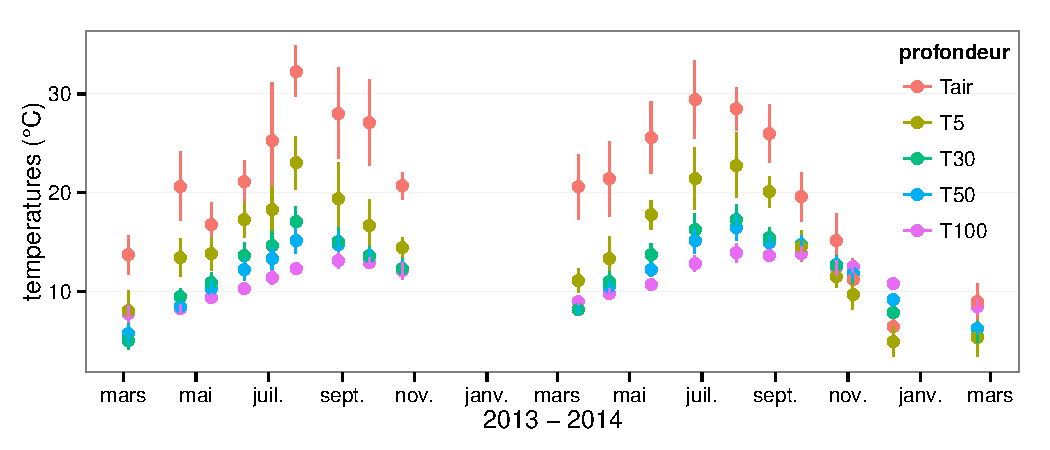
\includegraphics[width=1\textwidth, center]{chap3/T_mean_evolution}
\caption{Variabilité temporelle des moyennes des températures de l'air et du sol à \SIlist{-5;-30;-50;-100}{\centi\metre} mesurées dans les 20 placettes entre mars 2013 et février 2015}
\label{fig:T_mean_evolution}
\end{figure}

La température de l'air mesurée manuellement dans les 20 placettes montre une variabilité saisonnière comprise entre 6 et \SI{32}{\degreeCelsius} cohérente avec celle mesurée par la station météorologique. 
La variabilité saisonnière de la température est également visible quand elle est mesurée dans le sol avec un amortissement et une diminution de la variabilité spatiale avec la profondeur : les températures varient de 5 à \SI{17}{\degreeCelsius} et de 8 à \SI{14}{\degreeCelsius} à \num{-30} et \SI{-100}{\centi\metre} respectivement (Figure~\ref{fig:T_mean_evolution}).

\begin{figure}
\centering
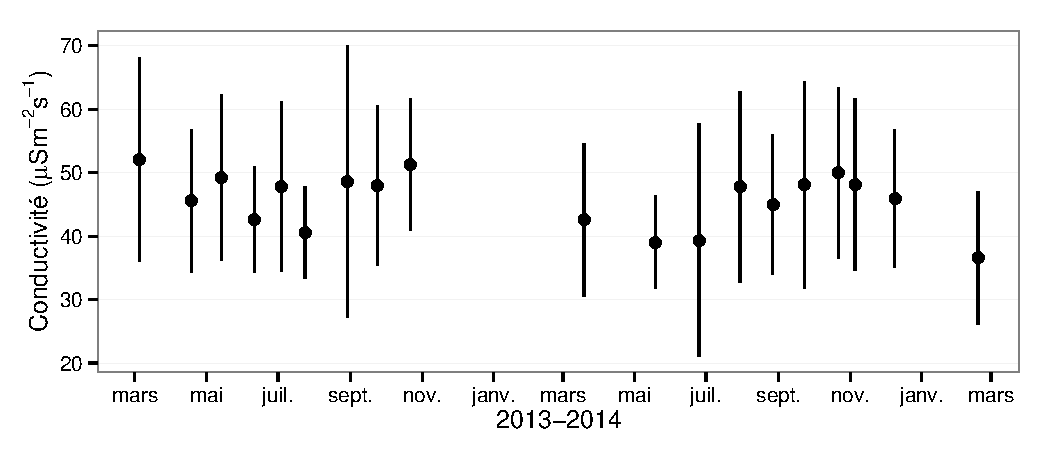
\includegraphics[width=1\textwidth, center]{chap3/cond_mean_evolution}
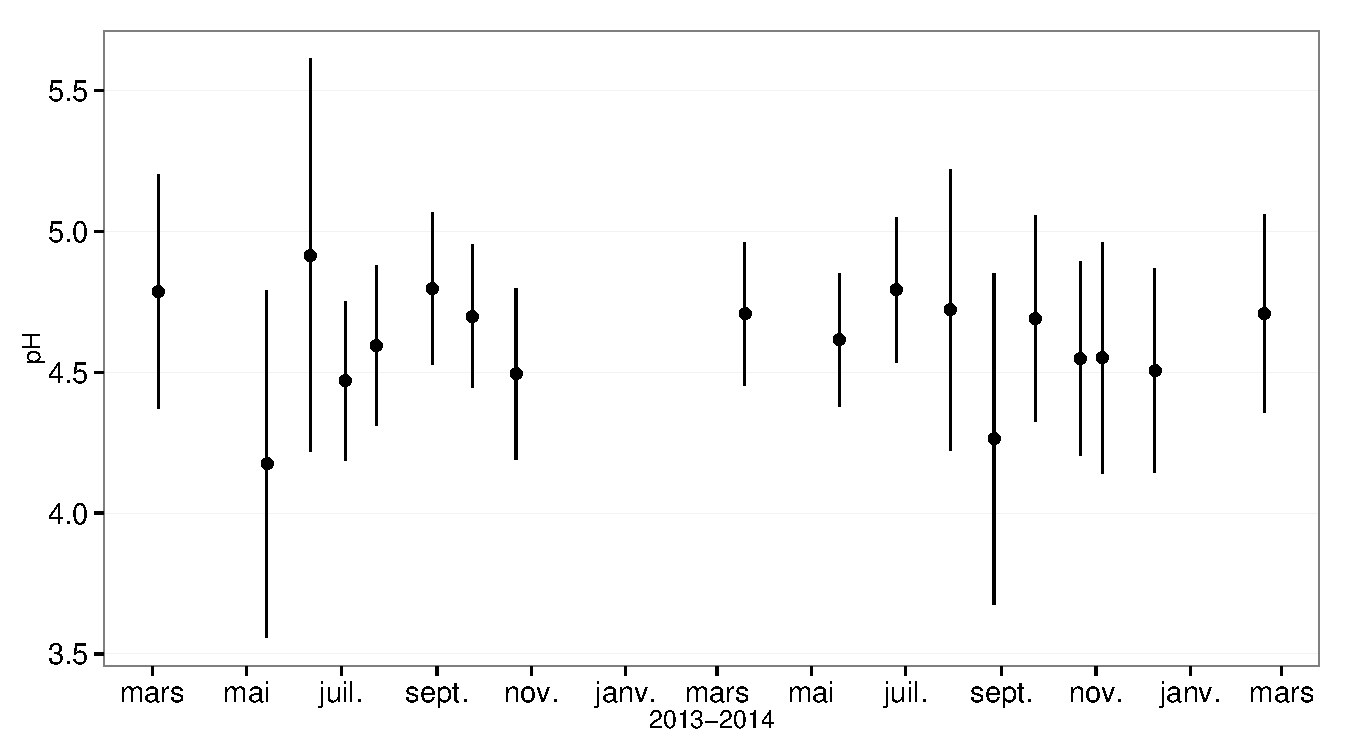
\includegraphics[width=1\textwidth, center]{chap3/pH_mean_evolution}
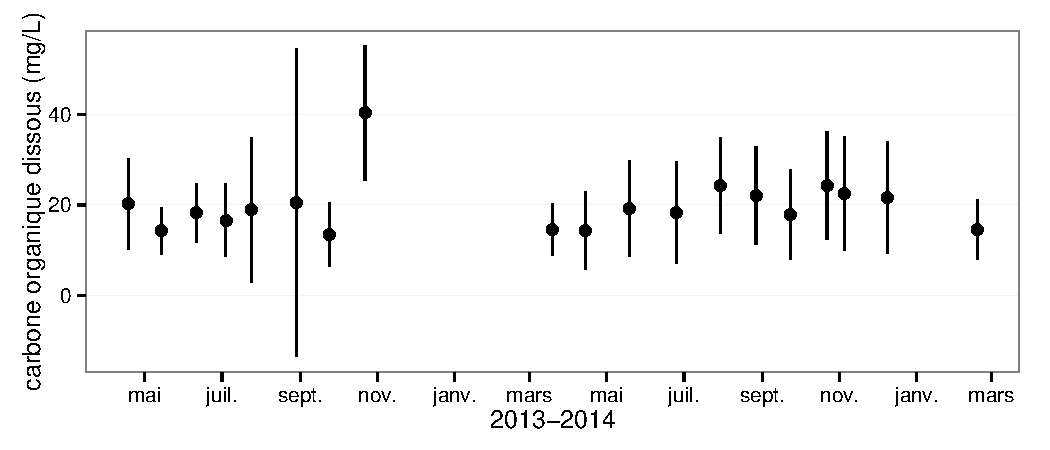
\includegraphics[width=1\textwidth, center]{chap3/NPOC_mean_evolution}
\caption{Variabilité temporelle des moyennes de la conductivité (A), du pH (B) et du carbone organique dissout (C) mesurés dans l'eau des piézomètres entre mars 2013 et février 2015.}
\label{fig:wtr_phychim}
\end{figure}

La conductivité moyenne mesurée dans l'eau des piézomètres des 20 placettes sur le site varie entre \num{35} et \SI{55}{\usml} (Figure~\ref{fig:wtr_phychim}--A).
En moyenne les valeurs de pH mesurées dans les placettes sont comprises entre 4 et 5 (Figure~\ref{fig:wtr_phychim}--B).
Ces valeurs sont cohérentes avec la classification en \textit{poor-fen} du site.
Les concentrations en carbone organique dissout des eaux prélevées dans les piézomètres sont comprises en moyenne entre \num{10} et \SI{30}{\milli\gram\per\liter} à l'exception d'un point en octobre 2013 (Figure~\ref{fig:wtr_phychim}--C).

\subsubsection{Flux de carbone}

\begin{figure}
	\centering
	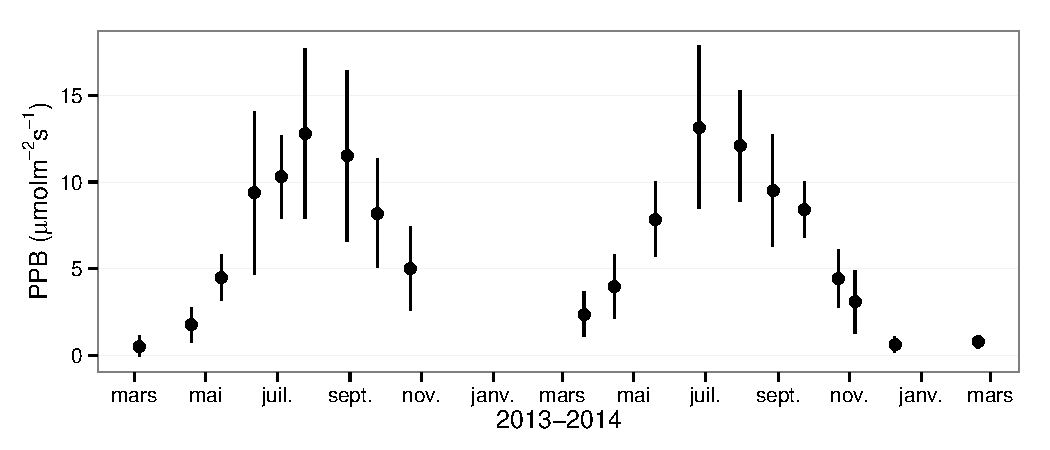
\includegraphics[width=1\textwidth, center]{chap3/GPP_evolution_avg}
	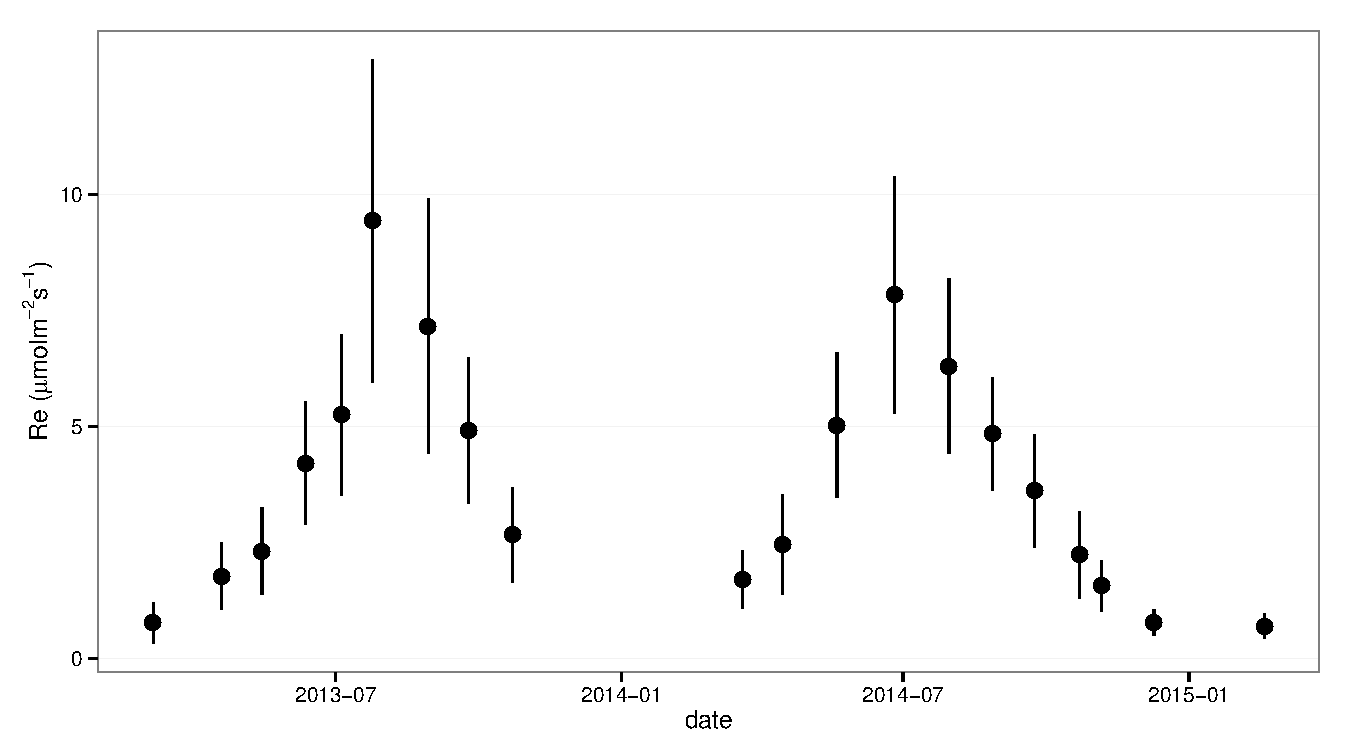
\includegraphics[width=1\textwidth, center]{chap3/ER_evolution_avg}
	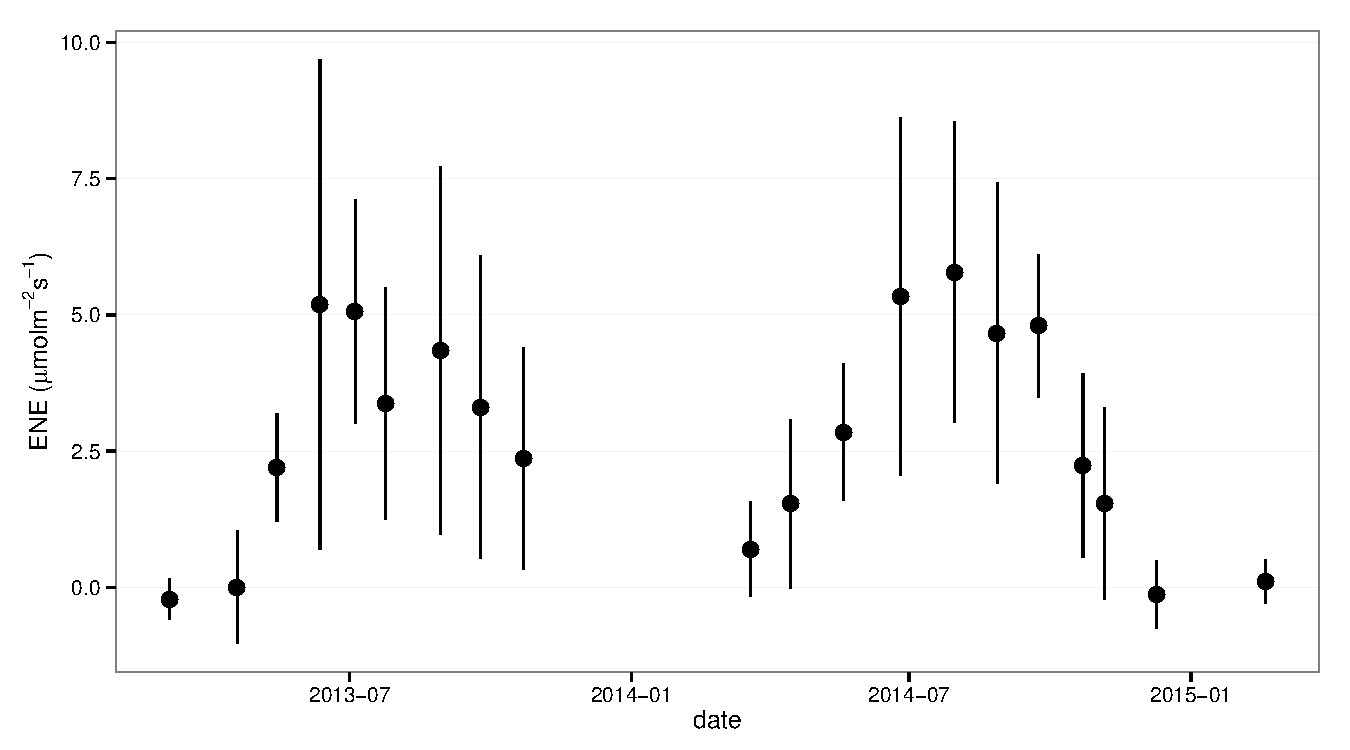
\includegraphics[width=1\textwidth, center]{chap3/NEE_evolution_avg}
\caption{Variabilité temporelle des flux de \coo moyen mesurés sur les 20 placettes entre mars 2013 et février 2015. Avec la PPB (A), la RE (B) et l'ENE (C) ; les barres d'erreur représentent l'écart type.}
\label{fig:flux_evolution_avg}
\end{figure}

Comme pour les variables environnementales, des mesures de \coo ont été effectuées de mars 2013 à février 2015.
De novembre 2013 à février 2014 les mesures ont été interrompues suite à des problèmes techniques.
Cependant les deux saisons de végétation ont pu être mesurées dans leur ensemble, permettant d'avoir un jeu de données représentatif sur le fonctionnement de l'écosystème.

En 2013, les valeurs de la \textbf{PPB} (flux de \coo entrant dans l'écosystème) augmentent au printemps et une partie de l'été avec un maximum de \SI{12.80(491)}{\uml} atteint fin juillet, avant de diminuer à partir d'août (Figure~\ref{fig:flux_evolution_avg}--A).
En 2014 la PPB maximale est atteinte fin juin (\SI{13.16(470)}{\uml}), soit environ un mois plus tôt que l'année précédente.
Pendant la deuxième partie de l'été et l'automne les valeurs décroissent jusqu'à être proches de 0.
En moyenne les valeurs de la PPB sont de \SI{7.12(519)}{\uml} en 2013 et de \SI{6.56(472)}{\uml} en 2014.

La \textbf{RE} (flux de \coo sortant de l'écosystème) en 2013 augmente pendant le printemps et une partie de l'été (Figure~\ref{fig:flux_evolution_avg}--B).
Elle atteint \SI{9.43(348)}{\uml}, son maximum, en juillet avant de diminuer.
En 2014 la RE atteint, comme la PPB, son maximum plus tôt, en juin avec une valeur moyenne de \SI{7.83(255)}{\uml} avant de décroître en automne et en hiver où elle approche de valeurs nulles.
Les valeurs moyennes de RE sont de \SI{4.27(316)}{\uml} en 2013, donc légèrement supérieures à celles de 2014 : \SI{3.63(256)}{\uml}.

En 2013 les valeurs de l'\textbf{ENE} (bilan des flux de \coo entrant et sortant, les valeurs négatives correspondent à une source de carbone et les valeurs positives à un puits) montrent un maximum en juin, atteignant \SI{5.19(451)}{\uml} puis elles diminuent jusqu'à la fin de l'année  (Figure~\ref{fig:flux_evolution_avg}--C).
Cependant, cette baisse est moins uniforme que celle des deux flux précédents, avec notamment une augmentation de l'ENE entre juillet et août 2013.
En 2014, l'ENE maximum est atteinte en juillet avec \SI{5.79(277)}{\uml}.
Les valeurs moyennes annuelles de l'ENE sont très proches et sont de \SI{2.85(305)}{\uml} pour 2013 et \SI{2.93(277)}{\uml} pour 2014.
À noter également que pour l'ensemble des flux, l'écart type augmente avec les valeurs mesurées.

Les flux de \textbf{\chh}, comme ceux du \coo, montrent une variabilité saisonnière importante, même si les flux de \chh mesurés sont un ordre de grandeur en dessous de ceux mesurés pour le \coo (Figure~\ref{fig:CH4_evolution_avg}).
À l'inverse de ce dernier, les flux de \chh mesurés en 2013 sont nettement inférieurs à ceux mesurés en 2014 avec une moyenne de \num{0.04(003)} et de \SI{0.10(008)}{\uml} respectivement.
Les valeurs moyennes maximales atteignent \num{0.078} en 2013 et \SI{0.196}{\uml} en 2014.

\begin{figure}
\centering
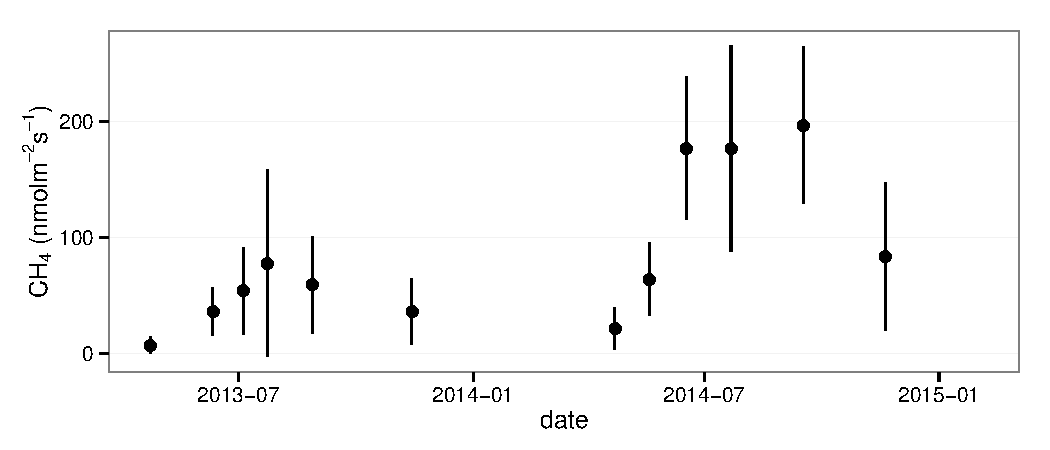
\includegraphics[width=1.15\textwidth, center]{chap3/CH4_evolution_avg}
\caption{Évolution des flux de \chh moyens sur cinq placettes entre mars 2013 et février 2015. Les barres d'erreur représentent l'écart type.}
\label{fig:CH4_evolution_avg}
\end{figure}

\subsubsection{Relations entre flux gazeux et variables environnementales}

\begin{figure}[!htb]
\centering
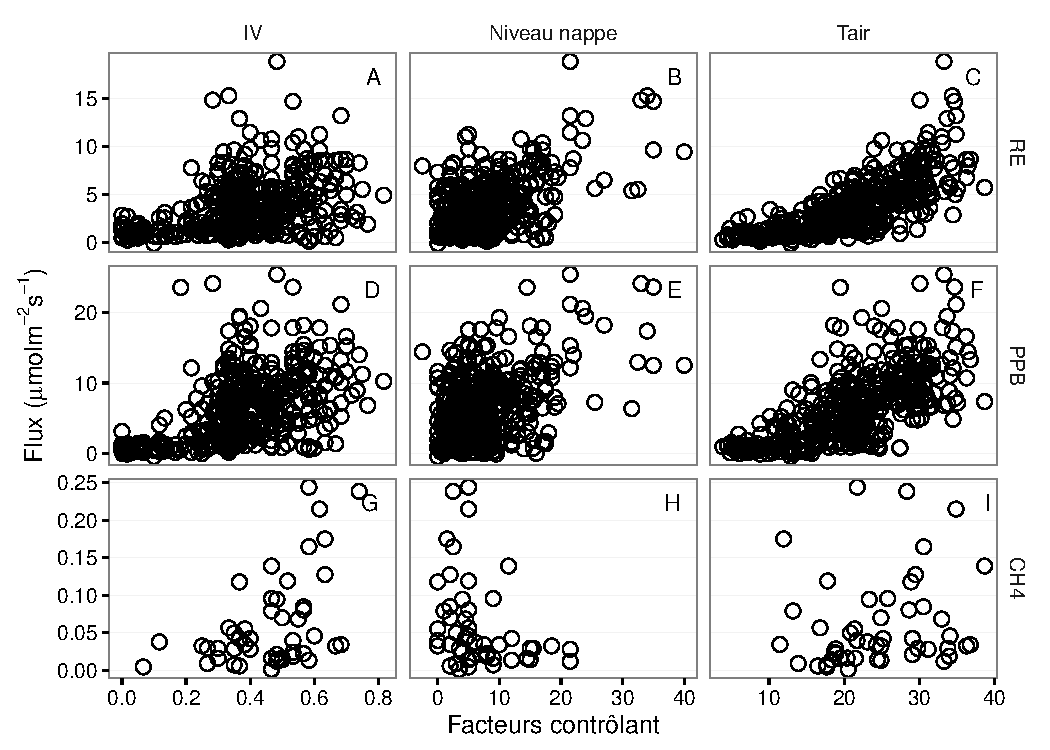
\includegraphics[width=\textwidth]{chap3/Fl_FC}
\caption{Relations entre les flux de gaz (exprimés en \si{\uml}) et une sélection de variables environnementales : l'indice de végétation à droite (IV, sans unité), le niveau de la nappe d'eau au milieu (cm) et la température de l'air (Tair en \si{\degreeCelsius})}
\label{fig:Fl_FC}
\end{figure}

Comme précisé précédemment, le niveau de la nappe d'eau a très peu varié pendant les deux années de mesures, hormis un faible étiage d'août à octobre 2013.
De ce fait aucune relation claire n'est identifiable entre les flux et le niveau de la nappe que ce soit pour le \coo (PPB et RE) ou le \chh (Figure~\ref{fig:Fl_FC}--B,E et H, coefficient de corrélation: r=0,5, r=0,4, et r=-0,3 respectivement).
La relation entre les flux de carbone (PPB et Re) et la température de l'air est de type exponentielle (Figure~\ref{fig:Fl_FC}--C et F, r=0,7 pour les deux).
Une tendance similaire est visible entre les flux de PPB et l'indice de végétation (IV), et dans une moindre mesure pour RE et \chh (Figure~\ref{fig:Fl_FC}--A,D et G, r=0,4, r=0,5 et r=0,5 respectivement).
Pour le \chh, aucune tendance n'est visible avec la température (r=0,2) ou le niveau de la nappe, même si pour ce dernier il semble y avoir un maximum d'émission entre 0 et \SI{-10}{\centi\metre}.
Les flux de \chh montrent une tendance exponentielle avec l'indice de végétation.

L'ensemble de ces observations sont cohérentes avec les résultats des ACP (Annexe~\ref{sec:carbiodiv}).

\subsection{Estimation des flux de GES}

\subsubsection{Production primaire brute}

L'estimation de la PPB se fait en deux étapes.
Dans un premier temps on estime le potentiel maximum de photosynthèse à un instant donné dans des conditions de lumière saturante (PPBsat).
Ce potentiel peut varier avec les conditions environnementales et a été déterminé en utilisant une équation qui relie la vitesse de transport des électrons photosynthétiques à lumière saturante à la température \citep{june2004} :

\begin{equation}\label{eq:juneTair}
PPBsat = a * exp\left(\frac{Tair - b}{c}\right)^2
\end{equation}

Avec :
\begin{itemize}
\item $a$ : vitesse de transport des électrons photosynthétiques à lumière saturante (\si{\uml})
\item $b$ : température optimale pour ce transport (\si{\degreeCelsius})
\item $c$ : différence de température à laquelle PBBsat vaut e$^{-1}$ de sa valeur à la température optimale (\si{\degreeCelsius})
\end{itemize}

À partir de ce potentiel à lumière saturante, la PPB est estimée en prenant en compte la luminosité.
On a utilisé l'équation~\ref{eq:PPB_bubier} proposée par \citep{bubier1998} et utilisée par de nombreux auteurs \citep{bortoluzzi2006a,worrall2009}:

\begin{equation} \label{eq:PPB_bubier}
PPB = \frac{PPBsat * i * PAR}{PPBsat + i * PAR}
\end{equation}

\begin{figure} %[!htb]
\centering
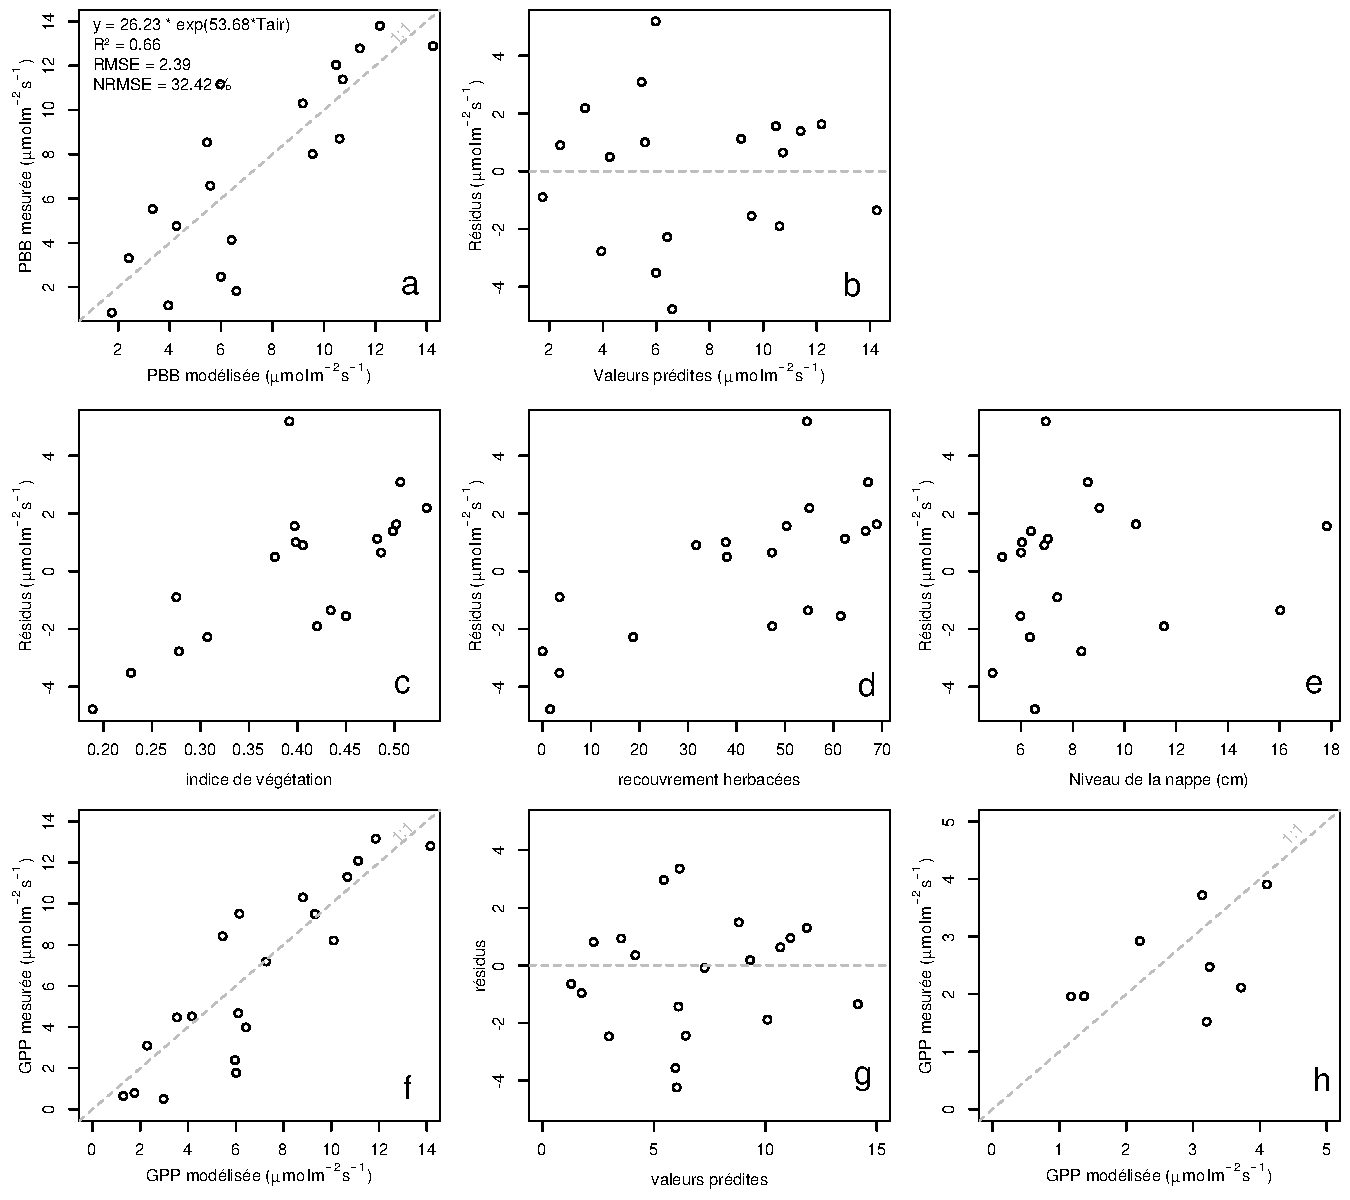
\includegraphics[width=1.15\textwidth, center]{chap3/mdl_GPP_Tair}
\caption{Résultats de la calibration de la PPB. En haut la PPBsat (équation~\ref{eq:juneTair} avec la représentativité du modèle et la distribution des résidus (graphes a et b). Au milieu les tendances entre les résidus de cette équation et l'indice de végétation, le pourcentage de recouvrement de la strate herbacée et le niveau de la nappe (graphes c, d et e). Et en bas la PPB (équation~\ref{eq:PPB_bubier}), sa représentativité et la distribution des résidus de l'équation (graphes f et g) et l'évaluation sur un jeu de données indépendant (graphe h, annexe~\ref{sec:carbiodiv}).}
\label{fig:mdl_GPP_Tair}
\end{figure}

L'utilisation de l'équation de June seule, avec la température de l'air comme variable explicative de la PPBsat, permet d'expliquer 66 \% des variations observées avec une NRMSE de \SI{32}{\percent} (Figure~\ref{fig:mdl_GPP_Tair}-a) et un AIC de 95 (Tableau~\ref{table:mdl_par}).
Les résidus de ce modèle se répartissent de façon relativement homogène et non biaisée (Figure~\ref{fig:mdl_GPP_Tair}-b).
Corrélés avec l'indice de végétation IV, ils présentent une tendance linéaire croissante (Figure~\ref{fig:mdl_GPP_Tair}-c).
On observe la même tendance avec le recouvrement de la strate herbacée avec une dispersion des points plus importante (Figure~\ref{fig:mdl_GPP_Tair}-d).
Par contre aucune relation n'est visible avec le niveau de la nappe d'eau (Figure~\ref{fig:mdl_GPP_Tair}-e).
Le pourcentage de recouvrement des sphaignes (non présenté) ne montre également aucune tendance avec les résidus de cette équation.
La PPB calculée à partir des équations~\ref{eq:juneTair} et \ref{eq:PPB_bubier} a une NRMSE de \SI{31}{\percent}, du même ordre de grandeur que celle de PPBsat (Figure~\ref{fig:mdl_GPP_Tair}-f) et les résidus se répartissent de façon relativement homogène et non biaisée (Figure~\ref{fig:mdl_GPP_Tair}-g).
Cependant l'évaluation du modèle sur les données de tests a une NRMSE plus forte qui atteint \SI{47}{\percent}(Figure~\ref{fig:mdl_GPP_Tair}-h).
Par ailleurs une forte incertitude est présente concernant l'estimation des paramètres qui ont tous une erreur standard importante (parfois plus importante que la valeur du paramètre) et une faible significativité (Tableau~\ref{table:mdl_par}).
Afin de prendre en compte la tendance linéaire entre les résidus et l'indice de végétation (IV) nous avons adapté le modèle, à la manière de \citet{bortoluzzi2006a}, pour y intégrer une fonction linéaire de la végétation :

\begin{equation}\label{eq:juneTairIV}
PPBsat = (a * IV + d) * exp\left(\frac{T - b}{c}\right)^2
\end{equation}

\begin{figure} %[!htb]
\centering
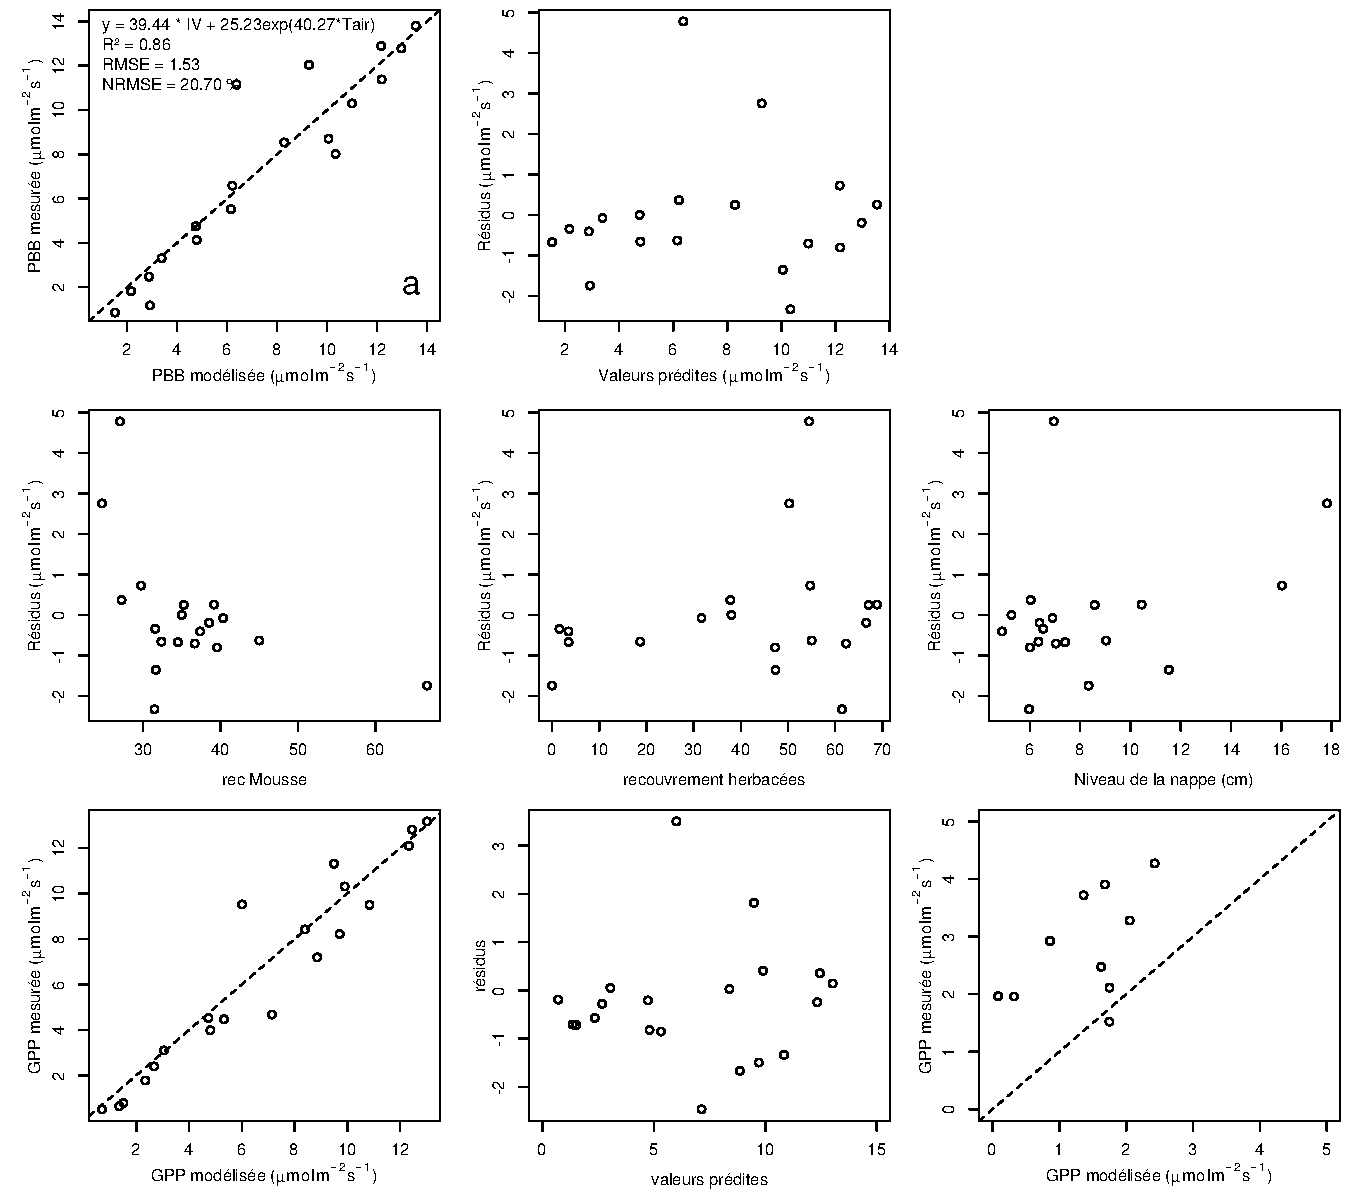
\includegraphics[width=1.15\textwidth, center]{chap3/mdl_GPP_TairIV}
\caption{Résultats de la calibration de la PPB en prenant en compte la végétation. En haut la PPBsat (équation~\ref{eq:juneTairIV} avec la représentativité du modèle et la distribution des résidus (graphes a et b). Au milieu les tendances entre les résidus de cette équation et l'indice de végétation, le pourcentage de recouvrement de la strate herbacée et le niveau de la nappe (graphes c, d et e). Et en bas la PPB (équation~\ref{eq:PPB_bubier}), sa représentativité et la distribution des résidus de l'équation (graphes f et g) et l'évaluation sur un jeu de données indépendant (graphe h, annexe~\ref{sec:carbiodiv}).}
\label{fig:mdl_GPP_TairIV}
\end{figure}

Cette nouvelle équation permet d'expliquer une part plus importante des variations de PPBsat (R$^{2}$ = 0,85) et augmente la proximité entre les données mesurées et les données modélisées : la NRMSE diminue à \SI{21}{\percent} (Figure~\ref{fig:mdl_GPP_TairIV}-a).
Par ailleurs son AIC est plus faible que pour l'équation précédente : 80 (Tableau~\ref{table:mdl_par}).
Les résidus de cette équation semblent répartis de façon moins homogène que précédemment.
Avec notamment un resserrement des points autour de zéro à l'exception d'un point de valeur supérieure à \num{4} (Figure~\ref{fig:mdl_GPP_TairIV}-b).
Le biais reste malgré tout faible au regard de l'amélioration apportée.
Aucune tendance claire ne se dégage des résidus lorsqu'ils sont mis en relation avec des variables telles que les recouvrements végétaux (que ce soit celui des sphaignes ou des herbacées), ou le niveau de la nappe d'eau (Figure~\ref{fig:mdl_GPP_TairIV}--c,d,e).
Comme précédemment, la NRMSE de la PPB, de \SI{19}{\percent}, est du même ordre de grandeur que celle de PPBsat (Figure~\ref{fig:mdl_GPP_TairIV}--f).
La NRMSE de PPBsat et PPB diminue avec la prise en compte de l'indice de végétation lors de la calibration.
En revanche, l'évaluation sur les données de test de ce dernier modèle montre une NRMSE importante (\SI{58}{\percent}), supérieure à celle du modèle ne prenant pas en compte la végétation (Figure~\ref{fig:mdl_GPP_TairIV}--h).
Cette évaluation montre également une tendance importante à sous-estimer les valeurs mesurées.
Néanmoins ce modèle, intégrant la végétation, permet de diminuer de façon importante l'erreur associée à l'estimation des paramètres de l'équation.

Dans la suite du texte le modèle permettant d'estimer la PPB à partir des équations~\ref{eq:juneTair} et \ref{eq:PPB_bubier} sera nommé \textbf{PPB-1} et celui utilisant les équations~\ref{eq:PPB_bubier} et \ref{eq:juneTairIV} sera nommée \textbf{PPB-2}.


\begin{table}
\centering
\caption{Valeur des paramètres des équations utilisées pour modéliser les flux et sensibilité relative (en \%) des flux en réponse à une variation de $\pm$\SI{10}{\percent} de chacun des paramètres des modèles.}
\label{table:mdl_par}
\begin{tabular}{llcccccc}\toprule

& par & valeur & se & pval & \SI{-10}{\percent} & +\SI{+10}{\percent} & AIC \\ \midrule
\multicolumn{7}{l}{PPB-1 -- équations~\ref{eq:juneTair} et \ref{eq:PPB_bubier}} & 95 \\ [+.5ex]
& a & 26.23 & 62.07 & 0.68 & -9.7 & +9.6 & \\
& b & 53.68 & 61.27 & 0.39 & +43.7 &-35.1 & \\
& c & 27.21 & 28.56 & 0.35 &-22.5 & +21.9 & \\
& i &  1.84 & 21.6  & 0.93 & -0.4 &  +0.4 & \\[+1ex]
\multicolumn{7}{l}{PPB-2 -- équations~\ref{eq:juneTairIV} et \ref{eq:PPB_bubier}} & 80 \\ [+.5ex]
& a & 39.44 & 18.89 & 0.05 & -11.8 & +11.5 &\\
& b & 40.27 & 19.11 & 0.05 & +15.8 & -17.2 &\\
& c & 25.23 & 14.35 & 0.1 & -8.1 & +6.7 &\\
& d & -3.73 & 3.49 & 0.3 & +2.8 & -2.8 &\\
& i &  0.26 & 0.25 & 0.31 & -1.3 & +1.1 &\\[+1ex]
\multicolumn{7}{l}{RE-1 -- équation~\ref{eq:RE_T}} & 47 \\ [+.5ex]
& a & 0.34 & 0.08 & 0 & -10 & +10 &\\
& b & 0.10 & 0.01 & 0 & -22.6 & +29.9 &\\[+1ex]
\multicolumn{7}{l}{RE-2 -- équation~\ref{eq:RE_TIV}} & 37 \\ [+.5ex]
& a & 0.92 & 0.34 & 0.02 & -7.3 & +7.3 &\\
& b & 0.09 & 0.01 & 0.00 & -19.5 & 24.7 &\\
& c & 0.14 & 0.09 & 0.14 & +2.7 & -2.7  &\\[+1ex]
\multicolumn{7}{l}{RE-3 -- équation~\ref{eq:RE_TH}} & 35  \\ [+.5ex]
& a & 0 & 0 & 0.01 & -3.9 & +3.9 &\\
& b & 0.08 & 0.01 & 0 & -18.8 & +23.6 &\\
& c & 0.33 & 0.06 & 0 & -6.1 & +6.1 &\\[+1ex]
\multicolumn{7}{l}{FCH4 -- équation~\ref{eq:CH4_H}}  &\\ [+.5ex]
& a & 0 & 0 & 0.48 & -10 & +10 &\\
& b & 13.01 & 2.82 & 0 & -43.9 & +79.2 & \\[+1ex]
\bottomrule
\end{tabular}
\end{table}

\subsubsection{Respiration de l'écosystème}

\begin{figure} %[!htb]
\centering
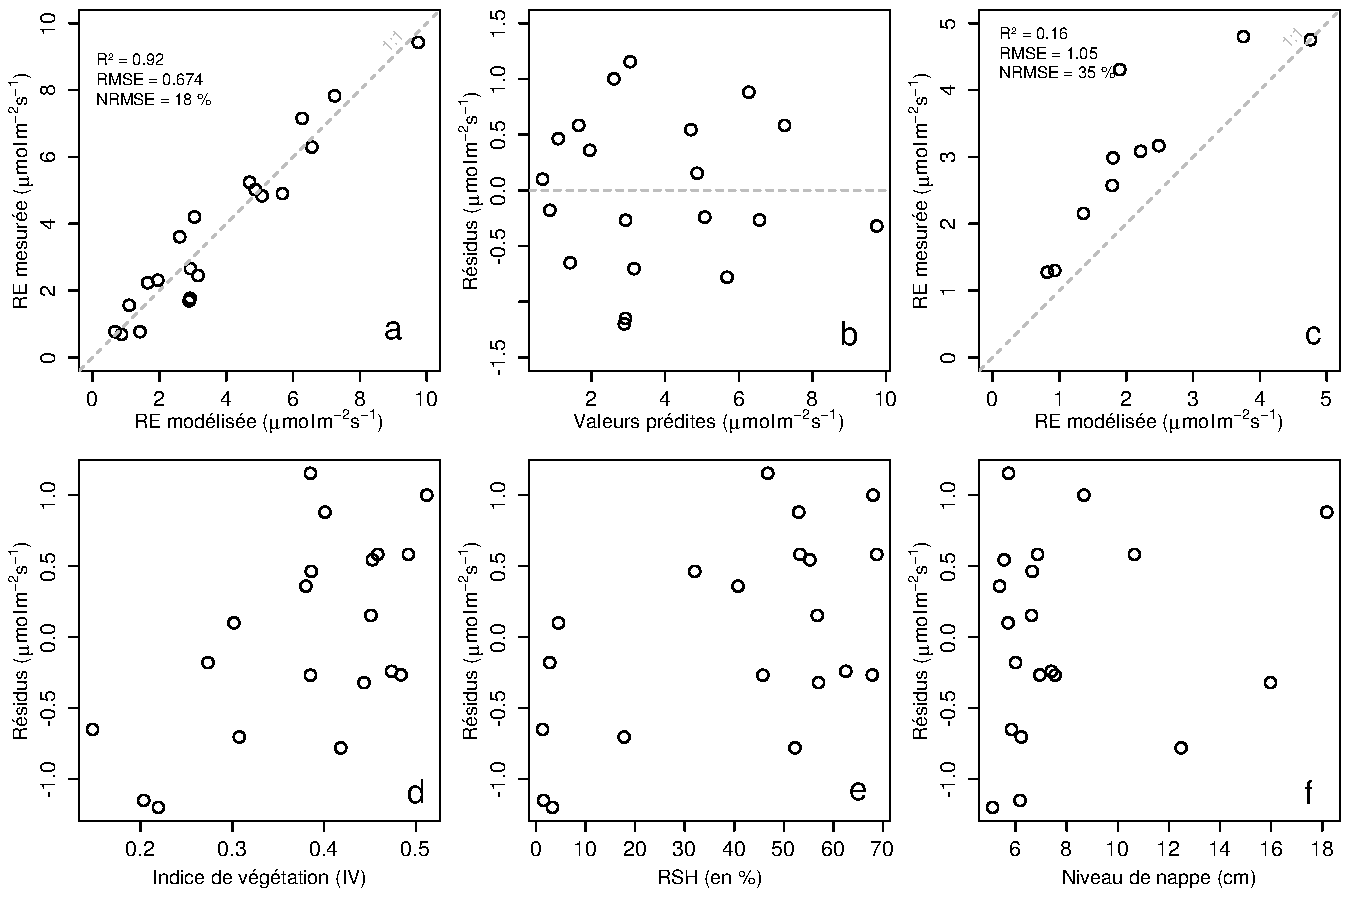
\includegraphics[width=1.05\textwidth, center]{chap3/mdl_ER_Tair}
\caption{\label{fig:mdl_ER_Tair}
Calibration de la RE utilisant l'équation~\ref{eq:RE_T}. En haut la représentativité du modèle et la distribution des résidus (graphes a et b), ainsi que son évaluation sur un jeu de données indépendant (graphe c, annexe~\ref{sec:carbiodiv}). En bas les tendances entre les résidus de cette équation et l'indice de végétation, le pourcentage de recouvrement de la strate herbacée et le niveau de la nappe (graphes c, d et e).}
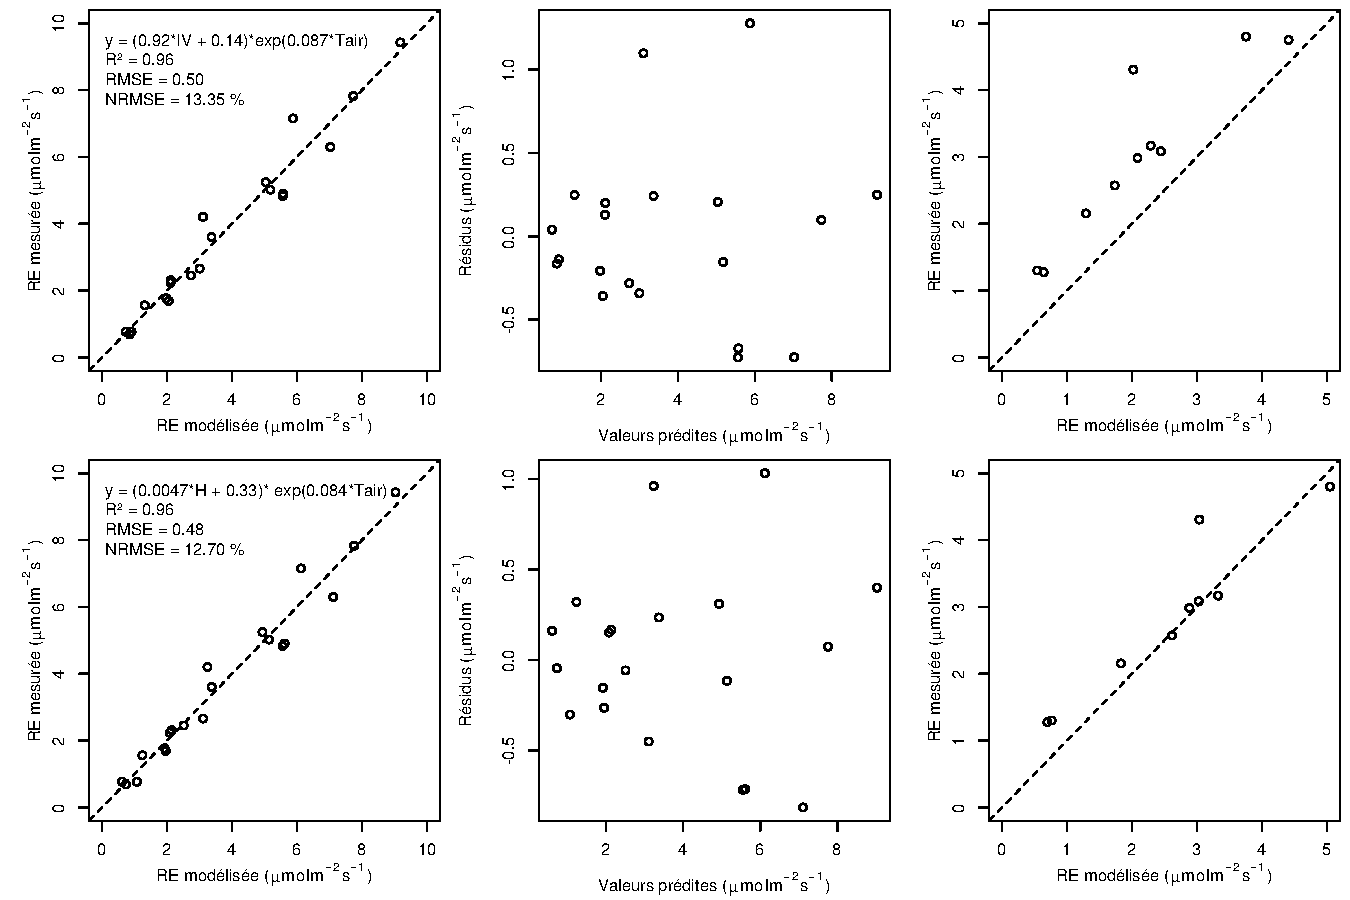
\includegraphics[width=1.05\textwidth, center]{chap3/mdl_ER_Tair_IVH}
\caption{\label{fig:ER_mdl_TairIVH}Calibration de la RE prenant en compte la végétation en utilisant l'équation~\ref{eq:RE_TIV}, en haut, et l'équation~\ref{eq:RE_TH} en bas. Avec la représentativité des modèles et la distribution de leurs résidus (graphes a et b pour le premier et d et e pour le second), ainsi que leur évaluation sur un jeu de données indépendant (graphe c et f, annexe~\ref{sec:carbiodiv}).}
\end{figure}

La relation exponentielle entre la RE et la température est reconnue \citep{luo2006}, et la RE est estimée avec l'équation :

\begin{equation} \label{eq:RE_T}
RE = a*exp(b*T)
\end{equation}

La température de l'air utilisée dans un modèle exponentiel permet d'expliquer \SI{90}{\percent} des variations de la respiration de l'écosystème avec une NRMSE de \SI{18}{\percent} (Figure~\ref{fig:mdl_ER_Tair}--a) et un AIC de 47.
Les résidus de cette équation sont répartis de façon non-biaisée (Figure~\ref{fig:mdl_ER_Tair}--b).
L'évaluation de ce modèle montre une NRMSE de \SI{35}{\percent} avec une tendance à sous-estimer les valeurs mesurées (Figure~\ref{fig:mdl_ER_Tair}--c).
Une légère tendance, est visible entre les résidus et l'indice de végétation ainsi qu'avec le recouvrement de la strate herbacée (Figure~\ref{fig:mdl_ER_Tair}--d,e) mais pas avec le niveau de la nappe (Figure~\ref{fig:mdl_ER_Tair}--f).
Très souvent utilisée, la température à \SI{-5}{\centi\metre} donne des résultats proches mais moins bons notamment avec une hétéroscédasticité des résidus (Annexe~\ref{sec:calib_flux}, figure~\ref{fig:RE_T5}).
On adapte l'équation~\ref{eq:RE_T} pour intégrer le signal de végétation de deux façon, avec l'IV :

\begin{equation} \label{eq:RE_TIV}
RE = (a*IV + c)*exp(b*T)
\end{equation}

Et avec le seul pourcentage de recouvrement des herbacées (RSH) qui contrôle en grande partie l'IV (Figure~\ref{fig:veg_evol})

\begin{equation} \label{eq:RE_TH}
RE = (a*RSH + c)*exp(b*T)
\end{equation}

Les calibrations de ces nouvelles équations sont présentées dans la figure~\ref{fig:ER_mdl_TairIVH}-a,b et \ref{fig:ER_mdl_TairIVH}-d,e respectivement.
Dans les deux cas, la NRMSE diminue pour avoisiner \SI{13}{\percent}, avec des résidus qui se répartissent de façon non-biaisée.
L'AIC diminue également jusqu'à 37 et 35 respectivement pour les équations~\ref{eq:RE_TIV} et \ref{eq:RE_TH}.
L'évaluation de ces deux équations montre cependant des différences :
d'une part l'équation~\ref{eq:RE_TIV} ne permet pas de diminuer la NRMSE (\SI{34}{\percent}) et est très proche des \SI{35}{\percent} calculés pour l'évaluation du modèle n'intégrant pas la végétation (Figure~\ref{fig:ER_mdl_TairIVH}--c).
D'autre part l'évaluation de l'équation~\ref{eq:RE_TH} montre une NRMSE plus faible de \SI{23}{\percent} (Figure~\ref{fig:ER_mdl_TairIVH}--f).
Les paramètres des différentes équations sont présentés dans le tableau~\ref{table:mdl_par} ; les modèles \textbf{RE-1}, \textbf{RE-2}, et \textbf{RE-3} correspondent respectivement aux équations~\ref{eq:RE_T}, \ref{eq:RE_TIV} et \ref{eq:RE_TH}.
À l'inverse de la PPB les paramètres des modèles de la RE ont, à l'exception du paramètre c du modèle RE-2, une significativité importante (p-value < 0,05) et une NRMSE faible (Tableau~\ref{table:mdl_par}).

\subsubsection{Flux de \chh}

\begin{wrapfigure}{r}[35pt]{0.55\textwidth}
\centering
\vspace{-40pt}
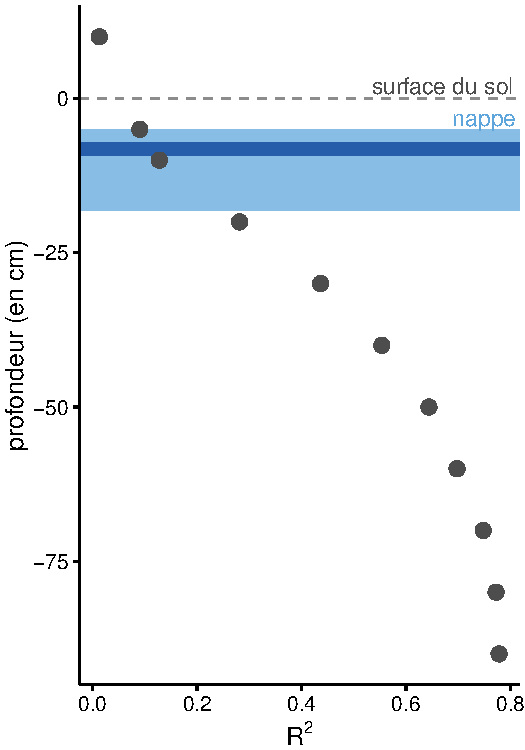
\includegraphics[width=.5\textwidth]{chap3/CH4_T_exp}
\caption{Évolution du R\textsuperscript{2} de l'équation $F_{CH_{4}} = a\times exp(b\times Temp\acute{e}rature)$ avec la profondeur. La ligne de tirets gris représente la surface du sol. La zone bleu clair représente la gamme des niveaux moyens relevés sur le site et la zone bleu foncé le niveau moyen pour l'année 2013 et 2014.}
\label{fig:CH4_T}
\end{wrapfigure}

Les relations entre les variables environnementales mesurées et les flux de \chh sont moins claires que celles concernant le \coo.
La corrélation la plus importante est liée à la végétation (Figure~\ref{fig:Fl_FC}).
Les flux de \chh ne montrent pas de tendance à augmenter de façon exponentielle avec la température de l'air.
Cependant cette relation se renforce d'autant plus que l'on utilise des températures mesurées à forte profondeur (Figure~\ref{fig:CH4_T}).
Souvent utilisées, les températures proches du niveau de nappe ont des R\textsuperscript{2} inférieurs à \num{0.50}.
Au delà, les R\textsuperscript{2} sont supérieurs à \num{0.50}, mais l'ensemble des placettes n'est plus représenté, certaines placettes n'ayant pas une épaisseur de tourbe supérieure ou égale à \SI{30}{\centi\metre}.
Le \chh ne montre pas de relation particulière avec le niveau de la nappe.
Les relations entre les flux de \chh et la végétation étant les plus significatives, elles ont été modélisées avec l'équation suivante :

\begin{equation} \label{eq:CH4_H}
F_{CH_{4}} = a*exp(b*IV)
\end{equation}

Avec les données acquises, l'indice de végétation est le meilleur prédicteur (Figure~\ref{fig:CH4_mdl}), car il explique \SI{78}{\percent} de la variabilité des flux \chh avec une NRMSE de \SI{32}{\percent} (Figure~\ref{fig:CH4_mdl}--a).
Aucune tendance ne semble se dégager entre les résidus de cette équation et les variables mesurées (Figure~\ref{fig:CH4_mdl}--d,e,f).

L'évaluation de cette équation montre une tendance à sous-estimer les flux de \chh et une NRMSE qui double par rapport à la phase de calibration en atteignant \SI{68}{\percent} (Figure~\ref{fig:CH4_mdl}--c).
Les détails de l'estimation des paramètres de l'équation~\ref{eq:CH4_H} sont visibles dans le tableau~\ref{table:mdl_par} sous le nom FCH4.

\begin{figure}
\centering
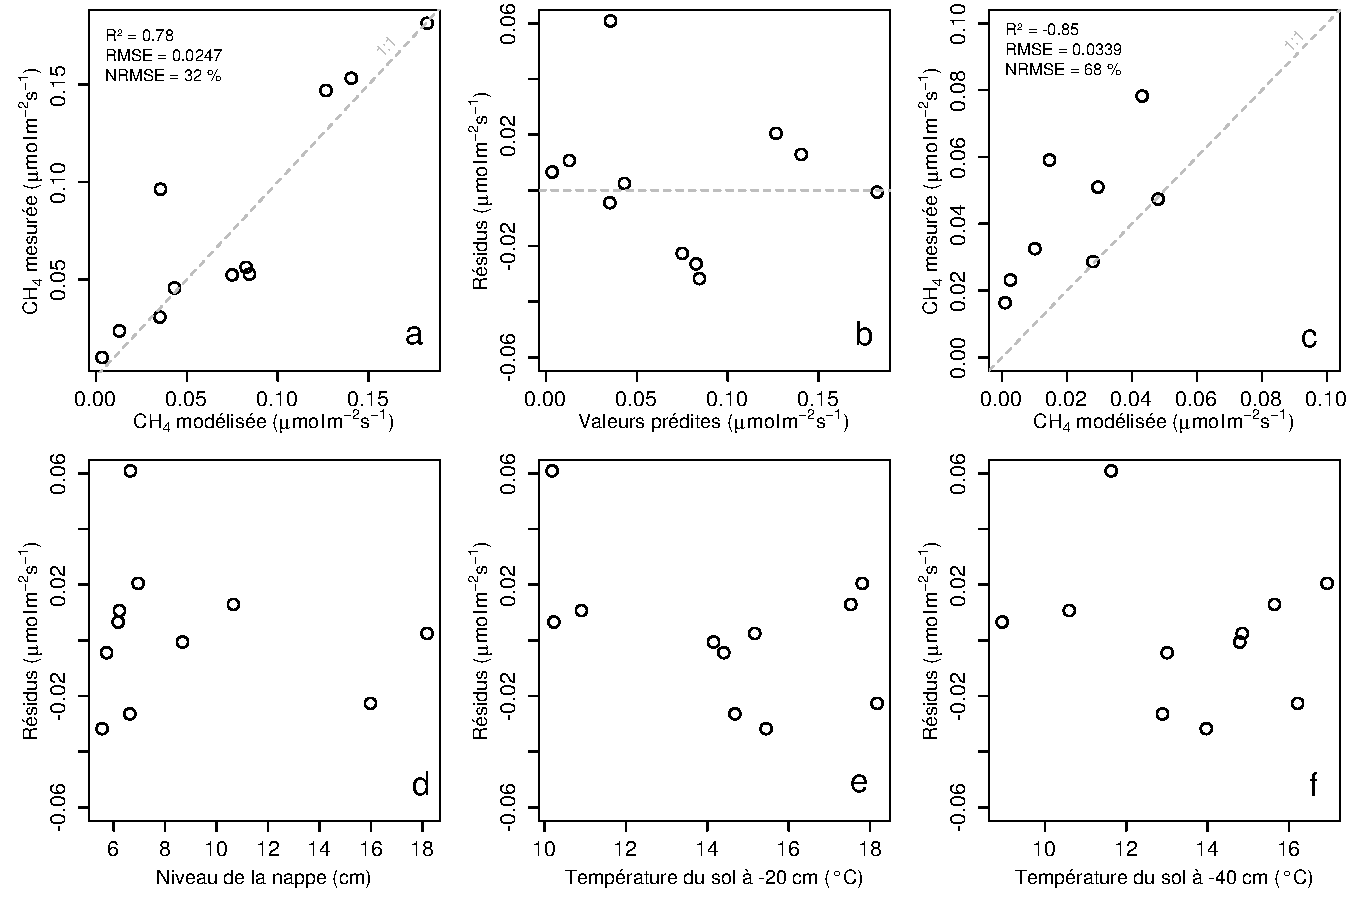
\includegraphics[width=1.15\textwidth, center]{chap3/mdl_CH4_IV}
\caption{Calibration des flux de \chh avec la végétation en utilisant l'équation~\ref{eq:CH4_H}. Avec la représentativité des modèles et la distribution des résidus de l'équation (graphes a et b), l'évaluation sur un jeu de données indépendant (graphe c) et les tendances des résidus de l'équation avec le niveau de la nappe la température du sol à \num{-20} et \SI{-40}{\centi\metre} (graphe d, e et f).}
\label{fig:CH4_mdl}
\end{figure}

\subsection{Le bilan de carbone à l'échelle de l'écosystème}

\begin{figure}[!hbt]
\centering
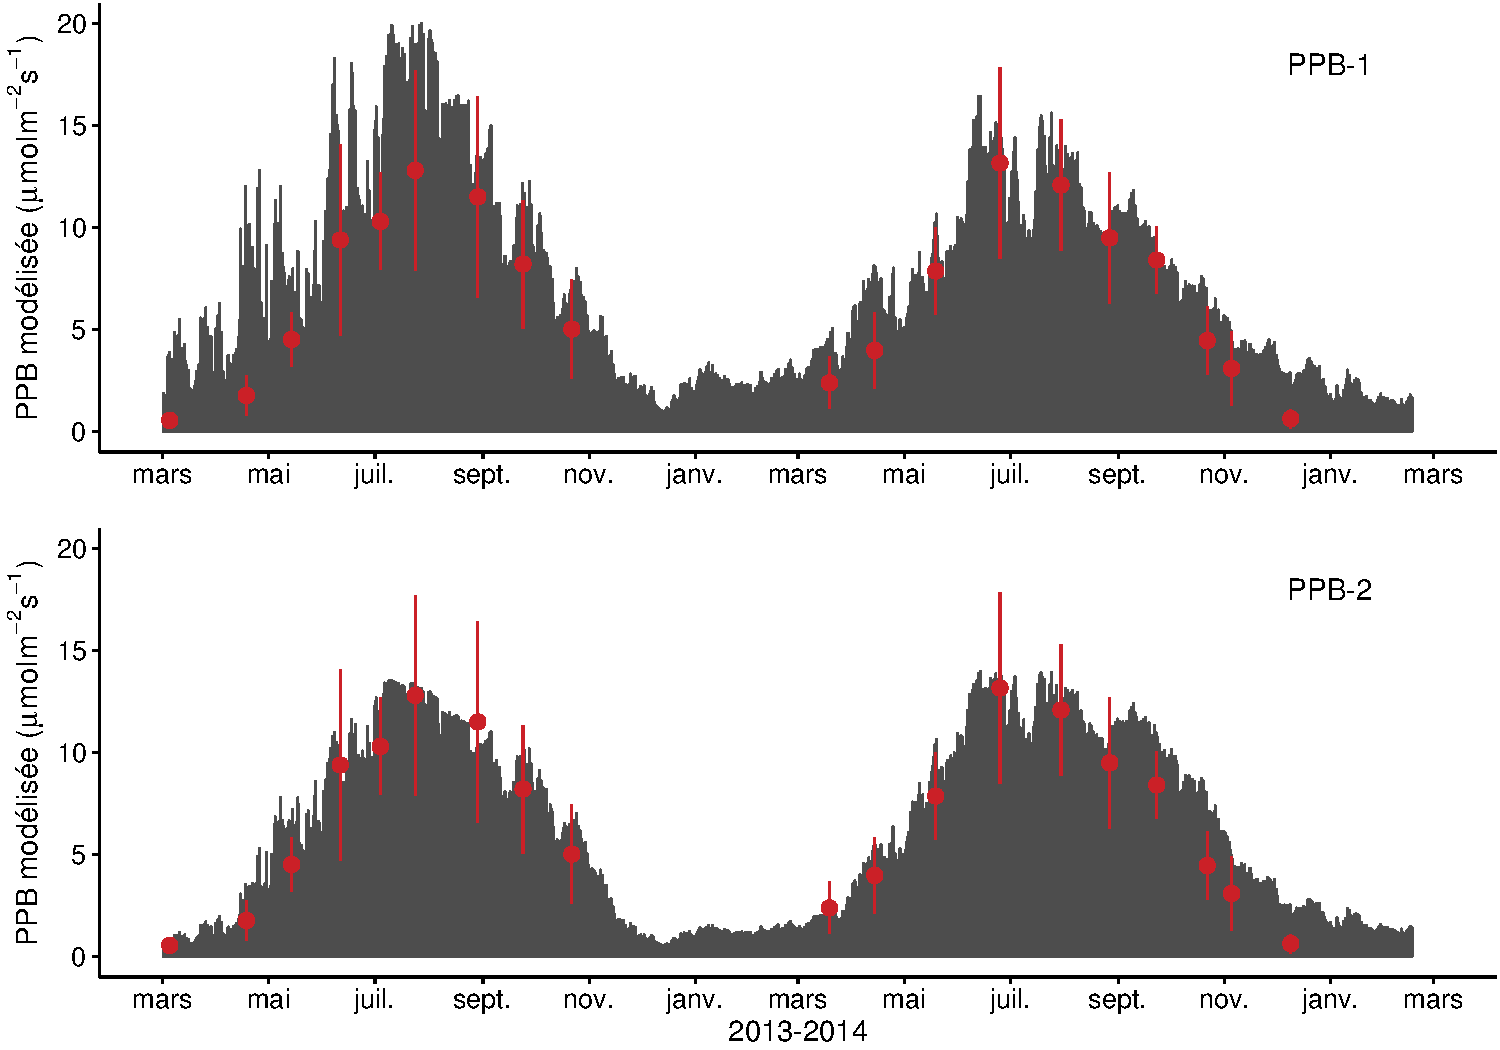
\includegraphics[width=1\textwidth, center]{chap3/BdC_GPP_interp}
\caption{Flux de \coo interpolé à l'heure à partir de PPB-1 (en haut) et PPB-2 (en bas). Les points rouges représentent les moyennes des mesures mensuelles et leur écart type}
\label{fig:BdC_GPP_interp}
\end{figure}

\begin{figure}
\centering
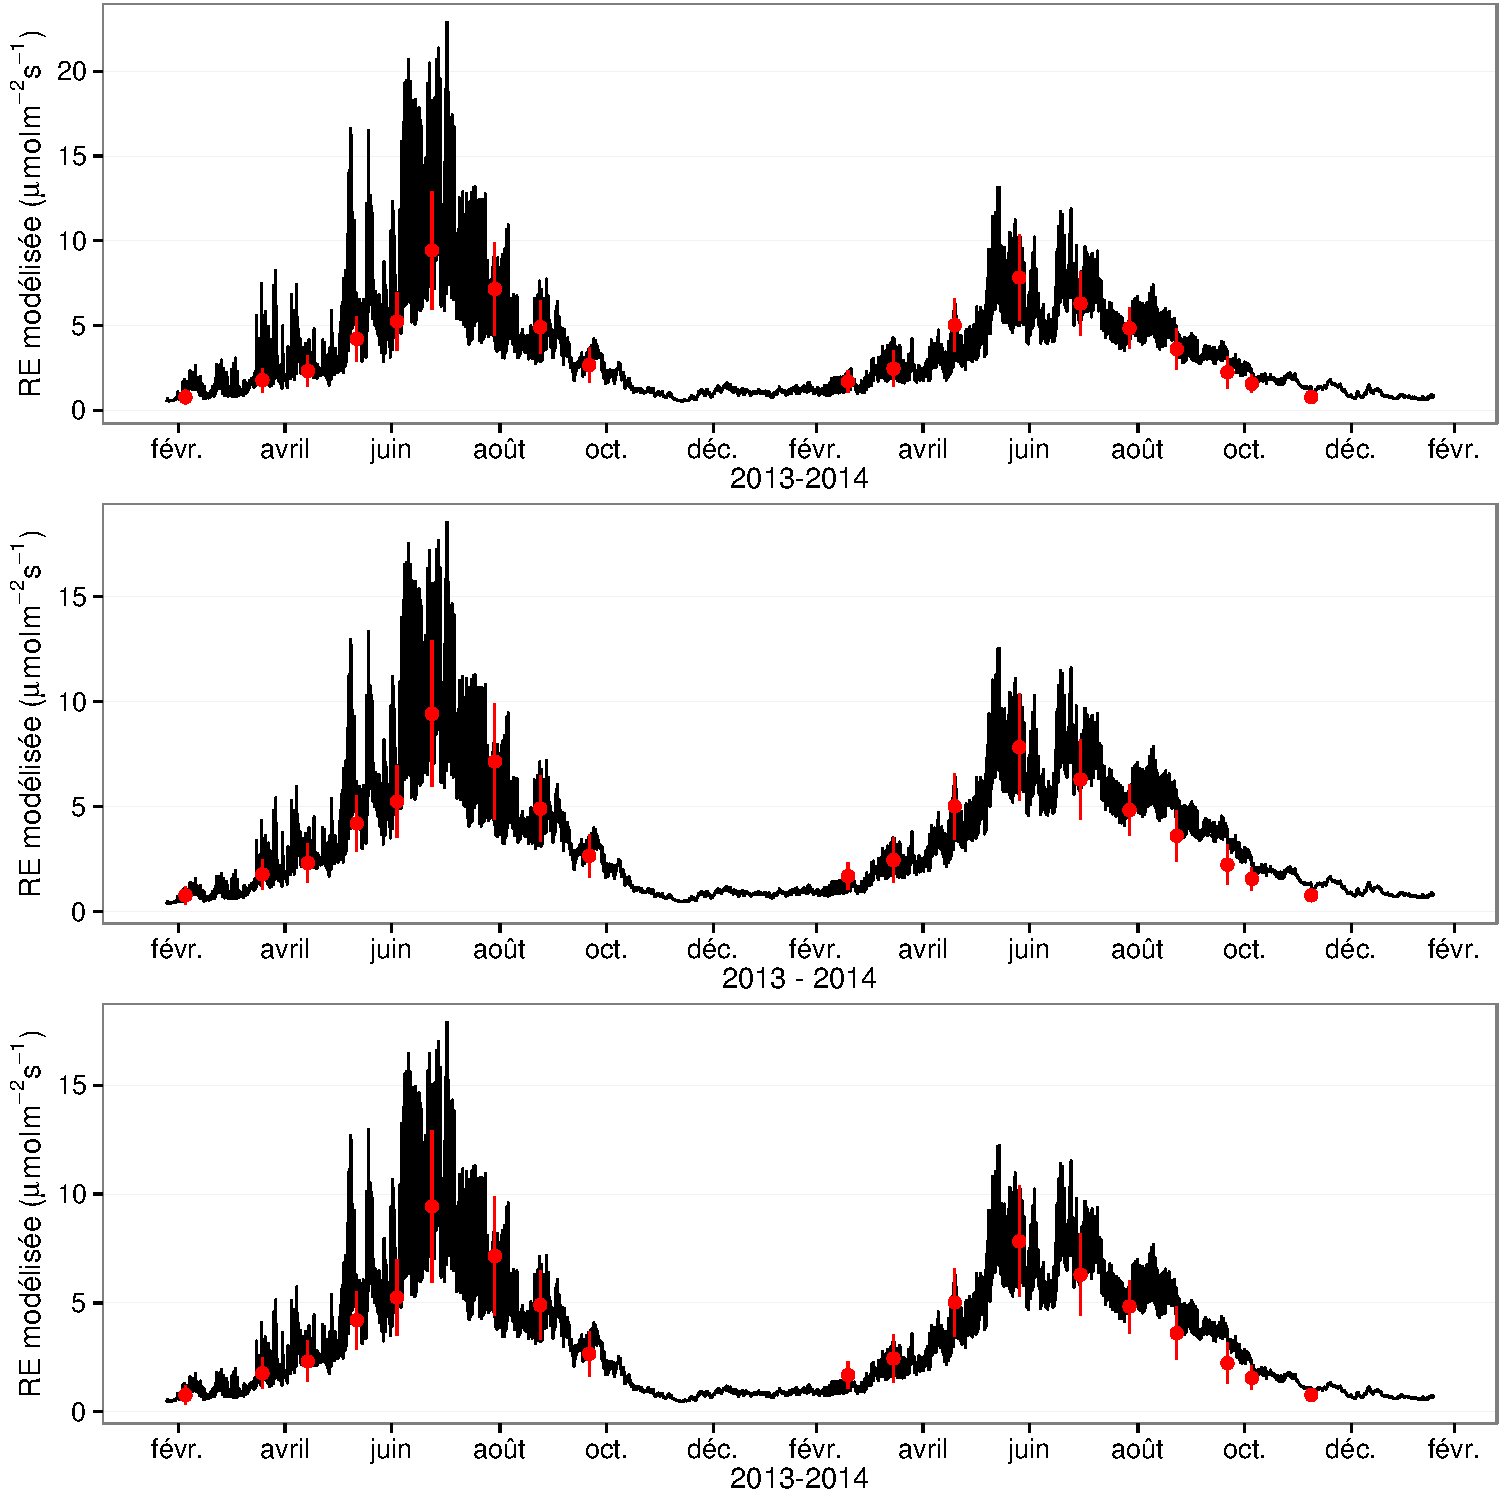
\includegraphics[width=1\textwidth, center]{chap3/BdC_ER_interp}
\caption{Flux de \coo interpolé à l'heure à partir de RE-1 (en haut), RE-2 (au milieu) et RE-3 (en bas). Les points rouges représentent les moyennes des mesures mensuelles et leur écart type}
\label{fig:BdC_ER_interp}
\end{figure}

\begin{figure}
\centering
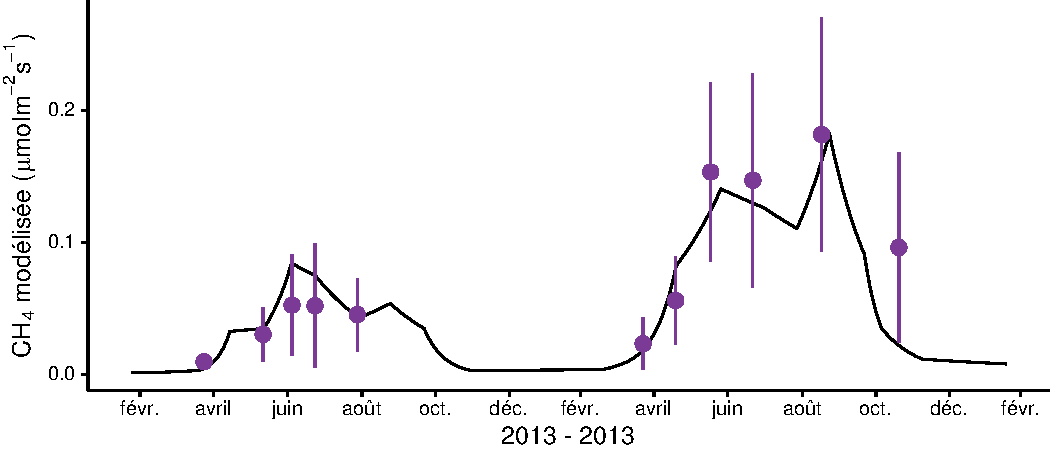
\includegraphics[width=1\textwidth, center]{chap3/CH4_BdCitp_IVcov}
\caption{Flux de \chh interpolé à partir de FCH4. Les points rouges représentent les moyennes des mesures mensuelles et leur écart type}
\label{fig:BdC_CH4_interp}
\end{figure}

Les interpolations des flux de PPB montrent une variabilité saisonnière proche de celle mesurée sur le terrain (Figure~\ref{fig:BdC_GPP_interp}). 
Les surfaces grises présentes sur la figure~\ref{fig:BdC_GPP_interp} sont liées au fait que la PPB tombe à zéro toutes les nuits.
Globalement le modèle PPB-2 semble mieux représenter les moyennes des flux mesurés sur le site.
Dans les deux cas les modèles semblent sur-estimer les valeurs de PPB mesurées fin 2014 et sous-estimer la PPB en été (en 2013 principalement pour PPB-1 et les 2 années pour PPB-2).

Pour la RE, l'interpolation reproduit également les variations saisonnières mesurées (Figure~\ref{fig:BdC_ER_interp}).
Les gammes de valeurs mesurées sont très proches des gammes interpolées :
les valeurs interpolées fluctuent dans les limites des barres d'erreurs.
L'interpolation des flux de la RE est très proche quel que soit le modèle utilisé (Figure~\ref{fig:BdC_ER_interp}).
L'intégration de la végétation dans les modèles RE-2 et RE-3 diminue les valeurs maximum de la RE modélisée en 2013 par rapport au modèle RE-1.

Les flux de \chh interpolés (Figure~\ref{fig:BdC_CH4_interp}) suivent également une cyclicité saisonnière.
Dans l'ensemble l'estimation du \chh semble rendre compte de la différence de flux mesuré en 2013 et en 2014.

La différence sur les cumuls quand les modèles de RE utilisent ou non la végétation est moindre : environ \SI{26}{\gcma} (tableau~\ref{table:bdc}).

\begin{table}
\centering
\caption{Cumul annuel des flux par année et moyen sur les deux années, en \si{\gcma}, en fonction des modèles utilisés. Les équations correspondent à celles détaillée dans le texte. L'incertitude associée à chaque flux est estimé à partir de la NRMSE.}
\label{table:flux}
\begin{tabular}{llllll}\toprule
Modèle & Flux & Équation(s) & 2013 & 2014 & Moyen \\ \midrule
PPB-1 & PPB & \ref{eq:juneTair} et \ref{eq:PPB_bubier} & 1322 $\pm$ 410 & 1258 $\pm$ 390 & 1290 $\pm$ 400 \\
PPB-2 & & \ref{eq:juneTairIV} et \ref{eq:PPB_bubier} & 957 $\pm$ 182 & 1184 $\pm$ 225 & 1070 $\pm$ 203 \\[+1.5ex]
RE-1 & RE & \ref{eq:RE_T} & 1337 $\pm$ 241 & 1235 $\pm$ 222 & 1286 $\pm$ 231 \\
RE-2 & & \ref{eq:RE_TIV} & 1232 $\pm$ 160 & 1310 $\pm$ 170 & 1271 $\pm$ 165\\
RE-3 & & \ref{eq:RE_TH} & 1240 $\pm$ 161 & 1281 $\pm$ 167 & 1261 $\pm$ 164 \\[+1.5ex]
FCH4 & CH4 & \ref{eq:CH4_H} & 10 $\pm$ 3 & 24 $\pm$ 8 & 17 $\pm$ 5 \\[+1.5ex]
FCOD & COD & \ref{eq:COD} & 8 $\pm$ 1  & 16 $\pm$ 1 & 12 $\pm$ 1 \\
\bottomrule
\end{tabular}
\end{table}

\begin{table}
\centering
\caption{Bilan de carbone annuel, en \si{\gcma}, en fonction des modèles utilisés. Les valeurs entre parenthèses représentent l'erreur associée au bilan (son calcul est décrit dans la partie~\ref{subsec:erreur_bilan})}
\label{table:bdc}
\begin{tabular}{llll}\toprule
combinaison de modèles & 2013 & 2014 & moyen \\ \midrule
PPB-1, RE-1, FCH4 &  \num{-33(6)} & \num{-18(0)} & \num{-26(4)} \\
PPB-1, RE-3, FCH4 &  +\num{64(16)} & \num{-64(11)} & +\num{0(3)} \\
PPB-2, RE-1, FCH4 &  \num{-398(70)} & \num{-91(14)} & \num{-245(44)} \\
PPB-2, RE-3, FCH4 &  \num{-301(47)} & \num{-138(20)} & \num{-220(33)} \\
\bottomrule
\end{tabular}
\end{table}

Les flux interpolés à une fréquence horaire puis sommés par année sont présentés dans le tableau~\ref{table:flux} pour les différents modèles utilisés.
Sur les deux années, selon le modèle utilisé, le flux total entrant via la PPB est estimé à 1070 et \SI{1290}{\gcma} pour PPB-2 et PPB-1 respectivement.
On observe une différence entre les deux modèles : 
celui utilisant uniquement la température de l'air (PPB-1) présente un stockage plus important en 2013 qu'en 2014, tandis que le modèle prenant en compte la végétation (PPB-2) stocke moins de carbone en 2013 qu'en 2014.
L'intégration de la végétation minimise également l'incertitude de l'estimation, la divisant approximativement par deux.

L'intégration de la végétation change également la différence entre 2013 et 2014 de la RE.
Lorsque la végétation est intégrée (RE-2 et RE-3) la RE est supérieure en 2014.
Lorsqu'elle ne l'est pas elle est supérieure en 2013.
Ces différences restent inférieures à l'incertitude liée aux flux estimés et on observe une grande proximité dans les valeurs des flux interpolés sur les 2 années, quel  que soit le modèle, avec un écart maximum de \SI{25}{\gcma}.

Les flux de \chh estimés ont une erreur importante et sont beaucoup plus faibles que les flux de la PPB ou de la RE.
Le flux de \chh est au moins deux fois plus important en 2014 qu'en 2013.

Les bilans issus des différentes combinaisons de modèles (à l'exception de RE-2, non présenté car très proche de RE-3) varient de \SI{-245(44)}{\gcma} à \SI{0(3)}{\gcma} stocké dans la tourbière (Tableau~\ref{table:bdc}).
L'intégration de la végétation dans la modélisation de PPB fait baisser les bilans de carbone dans le négatif (système source) au-delà de \SI{-200}{\gcma}, avec une différence entre les bilans de \SI{220}{\gcma} environ.

\subsubsection{Carbone organique dissout}

La quantité de COD sortant de la tourbière est estimée à \SI{8}{\gcma} en 2013 et \SI{16}{\gcma} en 2014 (Tableau~\ref{table:flux}).
Les concentrations moyennes en COD mesurées à l'exutoire sont très proches pour les deux années \num{18.6} et \SI{18.3}{\mgl} respectivement.
Par contre la quantité d'eau sortant de l'écosystème est plus importante en 2014 avec un export aux alentours de \SI{1000}{\cubic\metre} par jour entre octobre 2014 et février 2015 (Figure~\ref{fig:discharge}).

\begin{figure}
\centering
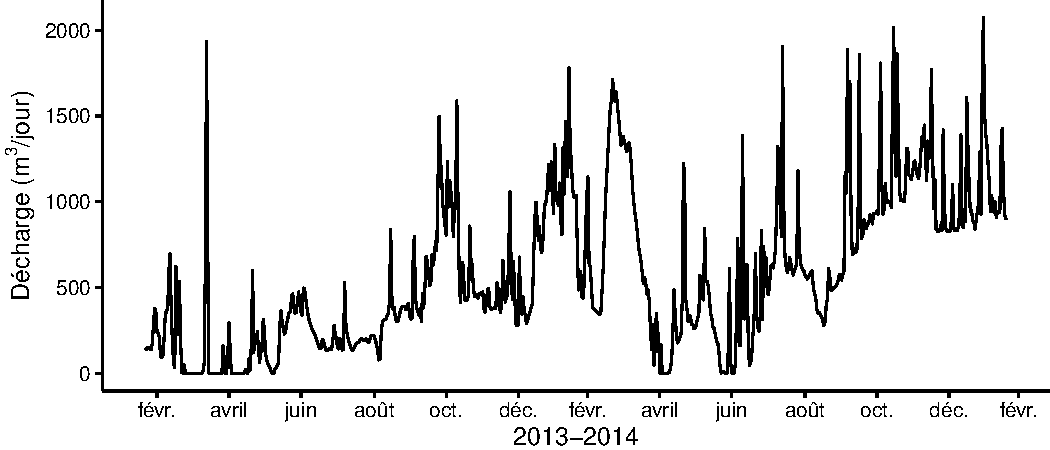
\includegraphics[width=1\textwidth, center]{chap3/discharge}
\caption{Quantité d'eau quittant le bassin versant de la tourbière, modifié d'après \citet{binet2013}.}
\label{fig:discharge}
\end{figure}

\subsubsection{Représentativité locale du bilan de \coo}

Il est possible d'avoir une indication sur la représentativité locale des modèles calibrés à l'échelle de l'écosystème en recalculant les flux mesurés sur chaque placette à l'aide des modèles en question et en recalculant une RMSE (Figure~\ref{fig:repr_loc}).

Que ce soit pour la PPB ou la RE, la placette n°5 a systématiquement une NRMSE significativement plus élevée que les autres (Figure~\ref{fig:repr_loc}).

Pour la PPB et si l'on excepte la placette n°5, les estimations à l'échelle de l'écosystème permettent de représenter les placettes avec une NRMSE comprise entre 20 et \SI{90}{\percent} pour PPB-1 et entre 30 et \SI{100}{\percent} pour PPB-2.
PPB-1 et PPB-2 ont une distribution des valeurs de NRMSE relativement similaire.

La NRMSE de RE-1 est comprise entre 20 et \SI{100}{\percent}, celle de RE-3 entre 20 et \SI{80}{\percent}.
La majorité des placettes ont une NRMSE d'environ \SI{55}{\percent} pour RE-1 et d'environ \SI{40}{\percent} pour RE-3 (Figure~\ref{fig:repr_loc}).
Le modèle RE-3 a des valeurs plus faibles et une distribution plus homogène de la NRMSE que RE-1, avec davantage de placettes en dessous de \SI{50}{\percent} (12 contre 8).

\begin{figure}
\centering
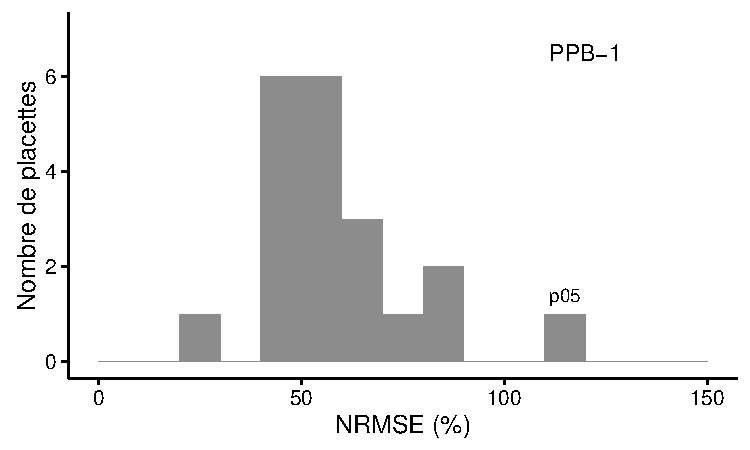
\includegraphics[width=.45\textwidth]{chap3/eco_to_loc_nrmse_PPB1}
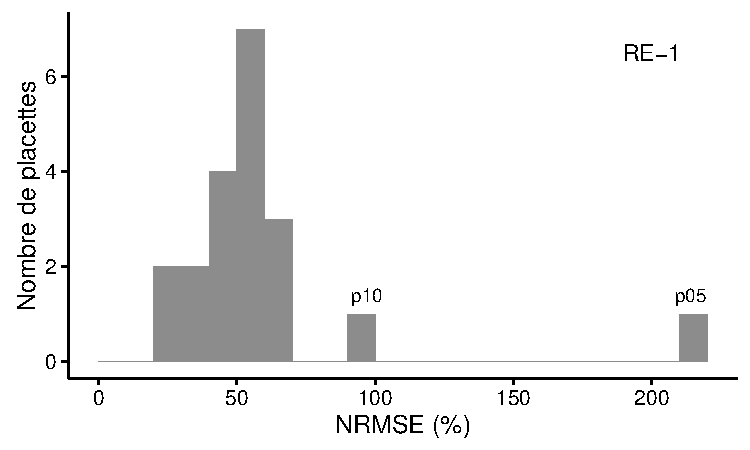
\includegraphics[width=.45\textwidth]{chap3/eco_to_loc_nrmse_RE1}\\
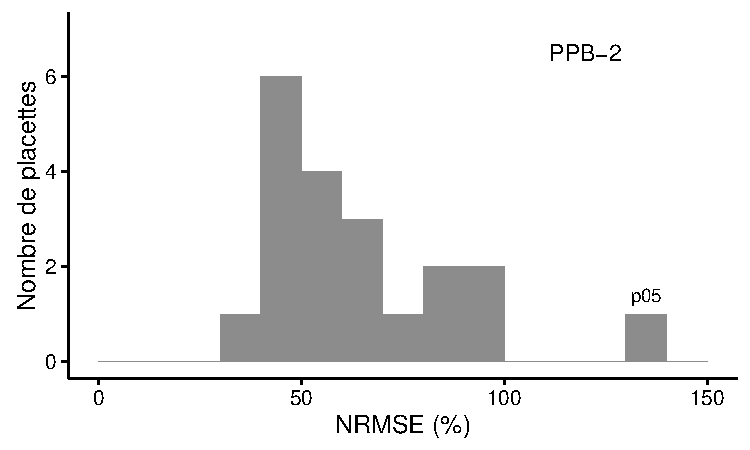
\includegraphics[width=.45\textwidth]{chap3/eco_to_loc_nrmse_PPB2}
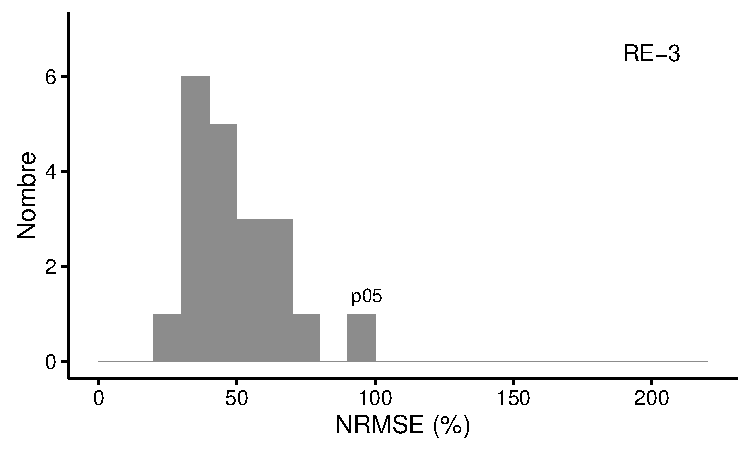
\includegraphics[width=.45\textwidth]{chap3/eco_to_loc_nrmse_RE3}
\caption{Distribution des valeurs de la NRMSE recalculée par placette à partir des modèles calibrés à l'échelle de l'écosystème}
\label{fig:repr_loc}
\end{figure}

\subsection{Variabilité spatiale du bilan de \coo}

\subsubsection{Calibration par groupe de placettes}

La classification hiérarchique a permis de distinguer 4 groupes de végétation (Figure~\ref{fig:tree}).
Dans le groupe Bryophytes, la strate muscinale est majoritaire avec un recouvrement moyen de \SI{91}{\percent}, et des recouvrements inférieurs à \num{35} et \SI{15}{\percent} pour les strates herbacées et arbustives respectivement (Figure~\ref{fig:distrib_grpveg}).
Le groupe Hétérogène est le plus homogène avec un recouvrement moyen des strates muscinales et arbustives de \num{63} et \SI{58}{\percent}.
C'est également le groupe dans lequel il y a le moins d'herbacées (\SI{24}{\percent}).
Dans le groupe Graminoïde, la strate herbacée est majoritaire avec un recouvrement moyen de \SI{63}{\percent}, la strate arbustive est moins présente (\SI{19}{\percent} en moyenne) et la strate muscinale est absente ($\approx$\SI{1}{\percent}).
La strate muscinale est également absente, dans le groupe Chaméphyte ligneux ($\approx$\SI{1}{\percent}), dans lequel la strate herbacée à un recouvrement de \SI{33}{\percent} et la strate arbustive de \SI{65}{\percent}.

Les flux, calculés pour chaque groupe à partir des même équations que celles utilisées à l'échelle de l'écosystème entier, ont des NRMSE plus importantes : de \num{41} à \SI{66}{\percent} pour RE-1 et RE-3 et de \num{39} à \SI{65}{\percent} pour PPB-1 et PPB-2 (Tableau~\ref{table:flux_grp}).

Les flux de RE estimés en regroupant les placettes selon leur végétation sont du même ordre de grandeur que ceux estimés pour l'ensemble de l'écosystème : entre \num{975(648)} et \SI{1453(740)}{\gcma} pour RE-1 et RE-3 (Tableau~\ref{table:flux_grp}).
Les groupes Hétérogène et Chaméphyte ligneux ont des flux similaires pour les deux modèles : \num{1365(670)} et \SI{1237(582)}{\gcma} pour RE-1 et \num{1393(681)} et \SI{1274(576)}{\gcma} pour RE-3.
Ces flux sont les plus proches de ceux estimés à l'échelle de l'écosystème (\num{1286(231)} et \SI{1261(164)}{\gcma} pour RE-1 et RE-3).
La prise en compte de la végétation (RE-3) fait diminuer fortement le flux estimé pour le groupe Graminoïde dont la RE passe de \num{1453(740)} à \SI{1115(455)}{\gcma}.
Parmi l'ensemble des groupes, le groupe Bryophytes à la RE la plus faible quel que soit le modèle considéré : \num{975(648)} et \SI{1023(439)}{\gcma} respectivement pour RE-1 et RE-3.

Concernant la PPB, les estimations des modèles calibrés par groupes sont inférieures à celles calculées à l'échelle de l'écosystème.
Ces relations sont à relativiser en considération des fortes incertitudes (Tableau~\ref{table:flux_grp}, annexe~\ref{sec:mdl_grp_veg}).
Ainsi les estimations par groupes de PPB-1 ont des valeurs comprises entre \num{886(501)} et \SI{1065(465)}{\gcma}, contre \SI{1290(400)}{\gcma} et les estimation de PPB-2 varient de \num{808(387)} à \SI{1277(642)}{\gcma}, par rapport à \SI{1070(203)}{\gcma} à l'échelle de l'écosystème.
Seules la PPB du groupe Graminoïde estimée avec PPB-2 est supérieure aux estimations faites pour l'ensemble des placettes.
À l'inverse de la RE, l'intégration de la végétation augmente, de \num{1056(682)} à \SI{1277(642)}{\gcma}, le flux du groupe Graminoïde.
En revanche, comme pour la RE, le groupe Bryophytes est celui dont les flux sont les plus faibles (\num{886(501)} et \SI{808(387)}{\gcma} pour PPB-1 et PPB-2).

Pour la PPB, les estimations de PPB-1 sont systématiquement inférieures à celles réalisées à l'échelle de l'écosystème.
Pour PPB-2 seul le groupe Graminoïde à une estimation supérieure.
Les différences entre PPB-1 et PPB-2 sont plus importantes que celles observées pour RE, même si la plus grande différence (\num{221}) est observée pour le même groupe, le groupe Graminoïde.
Le groupe Hétérogène a cependant une différence du même ordre de grandeur (\num{189}), tandis que pour les deux autres groupes cette différence est plus faible (78 et 58 respectivement pour les groupes Bryophytes et Chaméphyte ligneux).

\begin{figure}
\centering
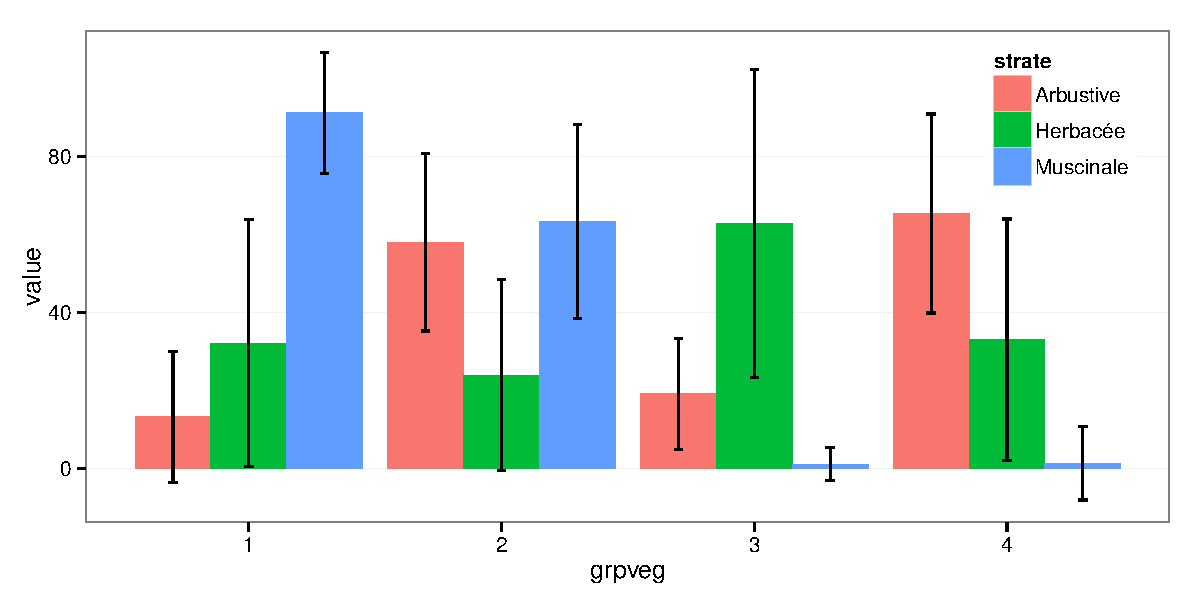
\includegraphics[width=\textwidth]{chap3/distrib_grpveg}
\caption{Recouvrement végétal moyen par strate (en \si{\percent}) des 4 groupes, les groupes sont nommés en fonction de la végétation majoritaire. Les barres d'erreur représentent l'écart type.}
\label{fig:distrib_grpveg}
\end{figure}

En termes de bilan de \coo, les groupes Chaméphyte ligneux et Bryophytes sont ceux qui sont le moins impactés par le choix des modèles (Tableau~\ref{table:bdc_grp}).
Quand la végétation n'est pas prise en compte pour l'estimation de la RE (modèle RE-1), le groupe Bryophytes est celui dont le bilan est le moins négatif.
Quand la végétation est prise en compte (modèle RE-3) c'est le groupe Graminoïde qui perd le moins de carbone (PPB-1, RE-3) voire qui en stocke (PPB-2, RE-3).
Les groupes Hétérogène et Chaméphyte ligneux ont des valeurs de bilan généralement proches quand la végétation n'est pas prise en compte dans l'estimation de la PPB.

\begin{table}
\centering
\caption{Cumul des flux de \coo en \si{\gcma} interpolés par groupe de végétation avec les modèles RE-1 et RE-3 pour la respiration et les modèles PPB-1 et PPB-2 pour la photosynthèse. (Le modèle RE-2, très proche de RE-3 n'a pas été inclus)}
\label{table:flux_grp}
\begin{tabular}{lllllll}\toprule
& \multicolumn{3}{c}{RE} &  \multicolumn{3}{c}{PPB} \\ \cmidrule(lr){2-4} \cmidrule(lr){5-7} 
groupe & valeur & R\textsuperscript{2} & NRMSE & valeur & R\textsuperscript{2} & NRMSE\\ \midrule
& \multicolumn{3}{l}{RE-1} &  \multicolumn{3}{l}{PPB-1} \\
Bryophytes &  \num{975} & \num{0.22} & \num{66.48} & \num{886} & \num{0.42} & \num{56.54} \\
Hétérogène &  \num{1365} & \num{0.58} & \num{49.09} & \num{1065} & \num{0.56} & \num{43.70}  \\
Graminoïde &  \num{1453} & \num{0.56} & \num{50.93}  & \num{1056} & \num{0.42} & \num{64.66} \\
Chaméphyte ligneux &  \num{1237} & \num{0.49} & \num{47.02} & \num{895} & \num{0.31} & \num{58.86}  \\ [+1ex]
& \multicolumn{3}{l}{RE-3} &  \multicolumn{3}{l}{PPB-2} \\
Bryophytes &  \num{1023} & \num{0.68} & \num{42.91} & \num{808} & \num{0.58} & \num{47.92} \\
Hétérogène &  \num{1393} & \num{0.58} & \num{48.88} & \num{876} & \num{0.65} & \num{38.93}  \\
Graminoïde &  \num{1115} & \num{0.72} & \num{40.84}  & \num{1277} & \num{0.65} & \num{50.30} \\
Chaméphyte ligneux &  \num{1274} & \num{0.53} & \num{45.25} & \num{953} & \num{0.46} & \num{52.14}  \\
\bottomrule
\end{tabular}
\end{table}

\begin{table}
\centering
\caption{Bilan de \coo par groupe de végétation (en \si{\gcma}) avec différentes combinaisons de modèles.}
\label{table:bdc_grp}
\begin{tabular}{lllll}  \toprule
Modèles & Bryophytes & Hétérogène & Graminoïde & Chaméphyte ligneux  \\ \midrule
PPB-1, RE-1 &  \num{-90(55)} & \num{-300(140)} & \num{-397(225)} & \num{-341(178)}\\[+1ex]
PPB-1, RE-3 &  \num{-138(67)} & \num{-328(153)} & \num{-59(31)} & \num{-378(193)} \\[+1ex]
PPB-2, RE-1 &  \num{-168(97)} & \num{-489(221)} & \num{-175(89)} & \num{-284(140)} \\[+1ex]
PPB-2, RE-3 &  \num{-216(97)} & \num{-517(233)} & +\num{162(74)} & \num{-321(155)} \\[+1ex]
\bottomrule
\end{tabular}
\end{table}

\subsubsection{Calibration par placette}


\begin{figure}
\centering
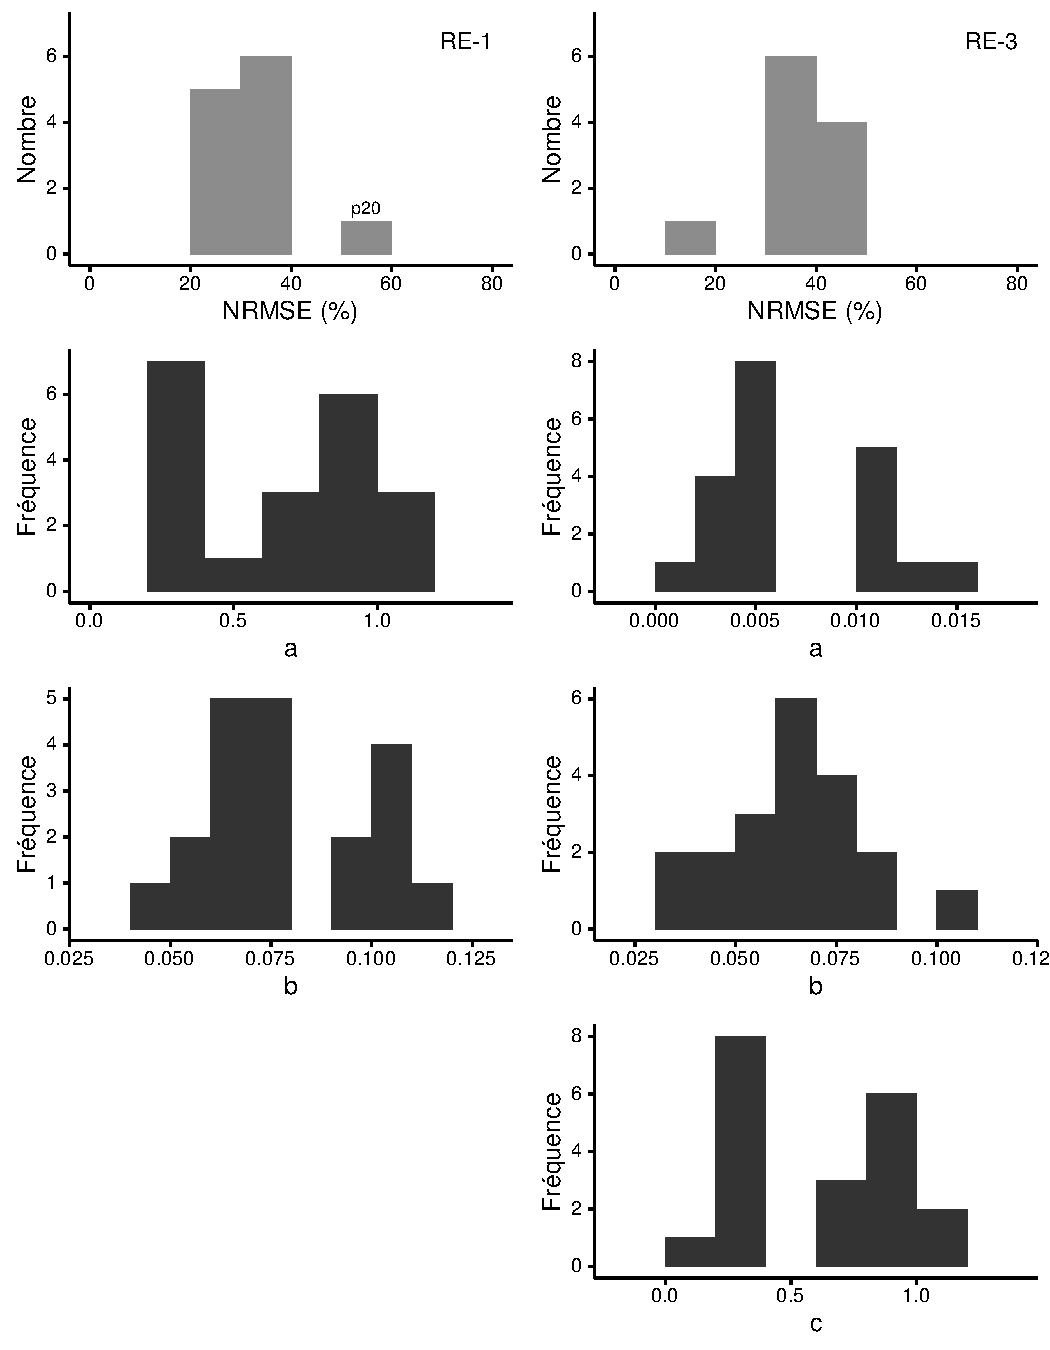
\includegraphics[width=.98\textwidth]{chap3/loc_ER}
\caption{Distribution de la NRMSE, du R\textsuperscript{2} (en gris) et des paramètres (en noir) des modèles RE-1 (à gauche) et RE-3 (à droite) calibrés par placette (N=20). Les lettres sous les graphes correspondent aux paramètres des équations utilisées.}
\label{fig:loc_ER}
\end{figure}

\begin{figure}
\centering
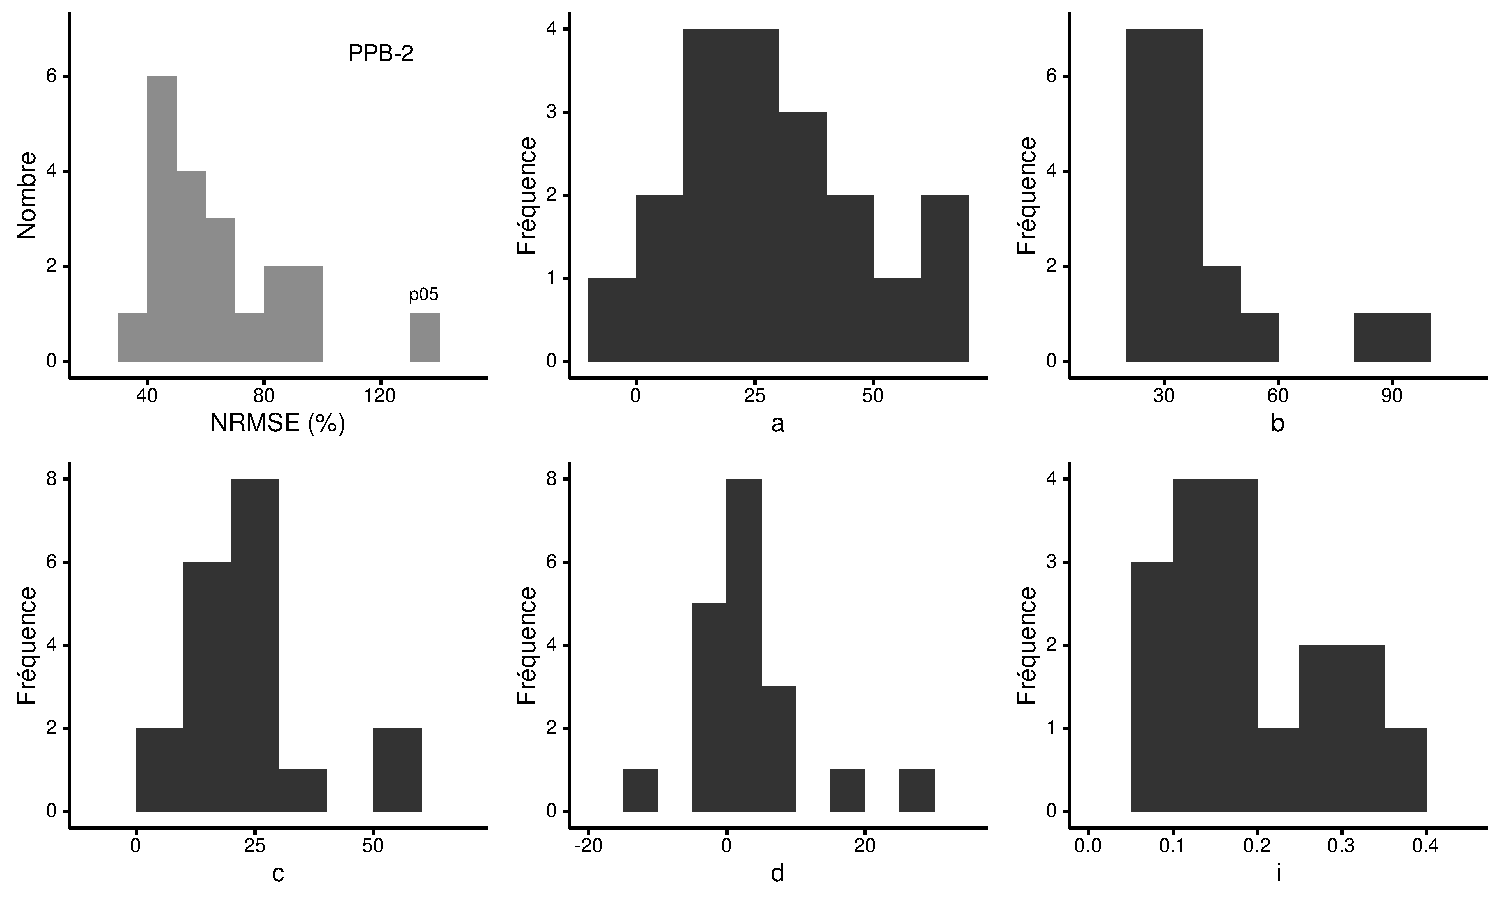
\includegraphics[width=1.15\textwidth, center]{chap3/loc_GPP}
\caption{Distribution de la NRMSE, du R\textsuperscript{2} (en gris) et des paramètres (en noir) du modèle PPB-2 calibré par placette (N=17). Les lettres sous les graphes correspondent aux paramètres des équations utilisées.}
\label{fig:loc_GPP}
\end{figure}

Les modèles RE-1, RE-3 ont pu être calibré pour l'ensemble des 20 placettes et le modèle PPB-2 pour 17 d'entre elles.
Le modèle RE-2, proche de RE-3 n'a pas été calibré.
Quant au modèle PPB-1, la calibration par placette ne convergeant pas pour la moitié d'entre elles, il n'a pas été pris en compte par la suite.
Il faut noter que la dispersion importante de points rend l'estimation des paramètres limitée en termes de significativité.
Par ailleurs que ce soit pour la PPB ou la RE, la placette n°10 semble avoir un comportement particulier.


Les R\textsuperscript{2} du modèle PPB-2, à l'exception de la placette n°10 , varient entre \num{0.5} et \num{0.9}.
La NRMSE se distribue entre 20 et \SI{60}{\percent}, ces valeurs sont supérieures à celles du modèle calibré à l'échelle de l'écosystème (\SI{19}{\percent}, Figure~ \ref{fig:ER_mdl_TairIVH}--d et \ref{fig:loc_GPP}).
Les paramètres du modèle PPB-2 varient de façon importante, entre \num{-6.1} et \num{66} pour a, entre \num{23.9} et \num{90.4} pour b, entre \num{6.2} et \num{60.0} pour c et \num{-10.7} et \num{27.1} pour d.

Toujours à l'exception de la placette n°10, pour les modèles RE-1 et RE-3 on constate une distribution des R\textsuperscript{2} au dessus de \num{0.5}, avec 11 placettes au dessus de \num{0.7} pour RE-1 et 15 pour RE-3.
Les valeurs de leurs NRMSE sont généralement plus élevées que celles obtenues à l'échelle de l'écosystème : entre 20 et \SI{55}{\percent} pour RE-1 (contre \SI{18}{\percent} à l'échelle de l'écosystème) et entre 15 et \SI{50}{\percent} pour RE-3 (contre \SI{13}{\percent}, Figure~\ref{fig:mdl_ER_Tair}--a, \ref{fig:ER_mdl_TairIVH}--d et \ref{fig:loc_ER}).
Les paramètres varient dans des gammes similaires pour RE-1 et RE-3 entre 0 et \num{1.1} pour a (RE-1) et a+c (RE-3) et entre \num{0.04} et \num{0.11} pour le paramètre b.


\begin{figure}
\centering
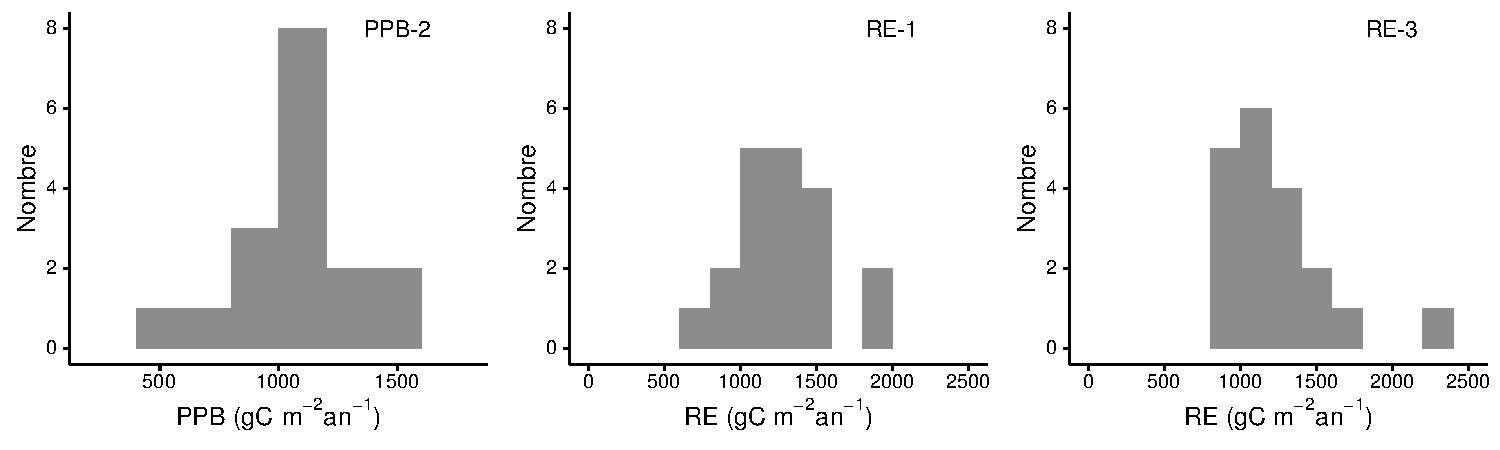
\includegraphics[width=1.15\textwidth, center]{chap3/distrib_flux_p7}
\caption{Distribution des flux estimés par placette en \si{gcma} pour le modèle PPB-2 (à gauche), RE-1 (au milieu) et RE-3 (à droite)}
\label{fig:distrib_fl_p7}
\end{figure}


Sur les deux années, les quantités de carbone assimilées par la PPB (modèle PPB-2) varient entre 507 et \SI{1409}{\gcma}, avec une majorité des placettes autour de \SI{1100}{\gcma} et une moyenne de \SI{1052(238)}{\gcma}.
Pour la RE, la distribution des flux du modèle RE-1 s'échelonne entre 633 et \SI{1832}{\gcma} avec une moyenne de \SI{1275(314)}{\gcma} et entre 828 et \SI{2371}{\gcma} avec une moyenne de \SI{1218(363)}{\gcma} pour le modèle RE-3.

Enfin la répartition spatiale des flux calculés par placette, que ce soit la PPB ou la RE, ne semble pas s'organiser suivant un gradient particulier (Annexe~\ref{sec:carte_flux}).

\section{Discussion}

La discussion de ce chapitre s'articule autour de quatre parties.
La première concerne les \textbf{modèles} calibrés à l'échelle de l'écosystème, leurs différences, leurs qualités respectives.
La seconde détaille les différents \textbf{flux} estimés par ces modèles.
Le(s) \textbf{bilan(s)} de carbone issu(s) de ces flux sont exposés dans la troisième partie.
Enfin, la quatrième partie porte sur la \textbf{variabilité spatiale} des flux.

\subsection{Modèles à l'échelle de l'écosystème}

\subsubsection{PPB}

À l'inverse du modèle PPB-2, le modèle PPB-1 ne prend pas en compte de façon directe la végétation.
L'estimation des paramètres de PPB-1, lors de la phase de calibration, conduit à une incertitude forte : l'erreur standard est supérieure à \SI{60}{\percent} pour les paramètres $a$ et $b$ et à \SI{20}{\percent} pour les paramètres $c$ et $i$ (Tableau~\ref{table:mdl_par}).
Cette incertitude diminue pour PPB-2 avec l'intégration de l'IV, l'erreur est alors inférieure à \SI{20}{\percent} pour l'ensemble des paramètres.
Ces paramètres sont dans la gamme de ceux rapportés par \citet{june2004} : entre \num{23} et \SI{296.5}{\umle} pour la vitesse de transport des électrons photosynthétique à lumière saturante, entre \num{28.4} et \SI{55.7}{\degreeCelsius} pour la température optimale du transport et entre \num{13.9} et \SI{30.2}{\degreeCelsius} pour la différence de température à laquelle PPBsat vaut e\textsuperscript{-1}.
Lors de la phase de calibration, l'intégration de l'IV augmente la significativité des estimations et la représentativité des données mesurées.

Lors de l'évaluation et malgré une végétation similaire, l'augmentation de la NRMSE du modèle PPB-2, intégrant l'IV, est supérieure et dépasse (en valeur absolue) celle du modèle PPB-1. 
L'apport de l'IV dans l'estimation de la PPB n'est donc pas pertinent pour le jeu de données indépendant utilisé.
Par ailleurs, l'intégration de l'IV à un effet beaucoup plus important en 2013 (l'estimation du flux diminue de \SI{365}{\gcma}), qu'en 2014 (diminution de \SI{74}{\gcma}).

Les différences observées selon la façon d'estimer la PPB peuvent paraître importante, néanmoins elles sont du même ordre de grandeur que celles rencontrées par \citet{worrall2009} qui comparent différentes approches pour modéliser des flux de gaz.

L'intégration de la végétation aux modèles d'estimation de la PPB est rarement réalisée \citep{bortoluzzi2006a,gorres2014}, probablement à cause de la difficulté à prendre en compte ce signal.
La diversité des espèces végétales rend difficile la mise en place de protocole de suivi non-destructif généralisable à un grand nombre d'espèces.

Il semble que le modèle PPB-2 soit le plus pertinent pour estimer la PPB sur la tourbière de La Guette.

\subsubsection{RE}

À l'inverse de la PPB, l'intégration de la végétation pour modéliser la RE améliore peu l'estimation de la RE lors de la phase de calibration : la différence entre les valeurs de la NRMSE est de \SI{5}{\percent} (Figures~\ref{fig:mdl_ER_Tair}--a et \ref{fig:ER_mdl_TairIVH}--a,d).
En revanche lors de la phase d'évaluation, l'utilisation du recouvrement des herbacées améliore l'estimation de façon plus importante avec une différence de \SI{11}{\percent} entre les valeurs de NRMSE.
La différence apportée par l'intégration de la végétation (RE-2 ou RE-3) est du même ordre de grandeur en 2013 et en 2014.
Sur les 2 années, l'effet de l'intégration de la végétation est limité avec une différence de \SI{25}{\gcma} au maximum (entre RE-1 et RE-3), soit moins de \SI{2}{\percent} du flux.
L'intérêt de l'évaluation pour la RE ne réside pas tant dans la sélection d'une meilleure estimation des flux.
Elle permet plutôt d'établir s'il est possible d'utiliser ou non un modèle dans un autre contexte.
Ainsi on peut envisager d'utiliser le modèle RE-3 sur d'autres données issues du même site.

Les incertitudes sur l'estimation des paramètres RE sont beaucoup moins importante que celles de la PPB.
L'estimation des paramètres des modèles, à l'exception du paramètre c du modèle RE-2, ont une p-value inférieure à 0,05 (Tableau~\ref{table:mdl_par}).
La NRMSE calculée lors de l'évaluation de ces modèles est certes plus importante que celle issue de la calibration, mais elle reste faible.
Ceci est particulièrement vrai pour le modèle RE-3 ou elle vaut moins de \SI{25}{\percent} (Figure~\ref{fig:ER_mdl_TairIVH}--f).
La RE semble donc mieux contrainte que la PPB, avec une estimation des paramètres plus fiable et une différence entre les estimations issues des différents modèles plus faible.

Le modèle RE-3 semble être le plus pertinent pour estimer la RE sur la tourbière de La Guette

\subsubsection{\fchh}

La calibration des flux de \chh conduit à une erreur du même ordre de grandeur que celle obtenue pour PPB-1 (Figure~\ref{fig:CH4_mdl}). 
L'évaluation du modèle fait doubler la NRMSE et montre sa limite : son utilisation est nécessairement restreinte à cette étude particulière.

\subsection{Les flux annuels à l'échelle de la tourbière de La Guette}

\subsubsection{Représentativité à l'échelle globlale}

\begin{figure}
\centering
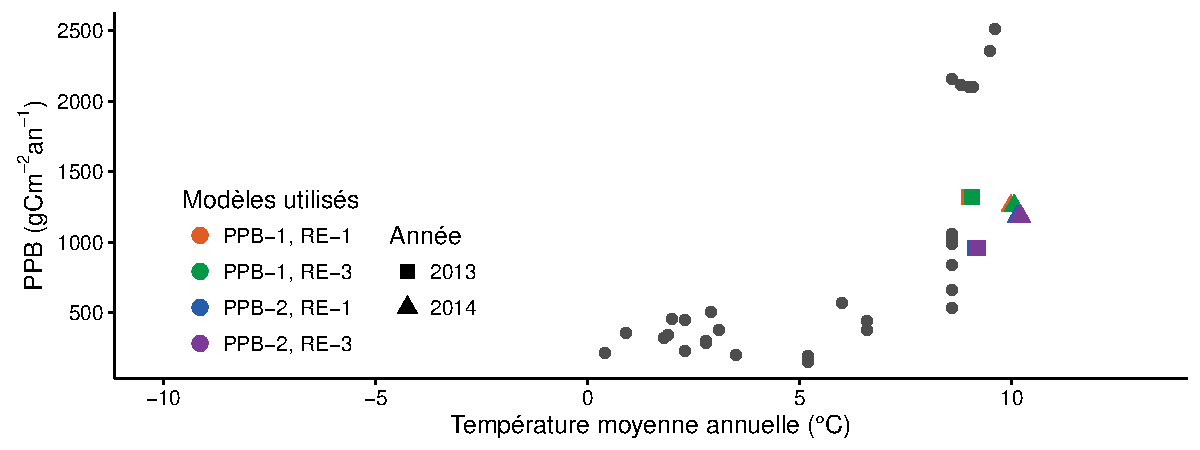
\includegraphics[width=\textwidth]{chap3/bib_vs_ppb}
\caption{Relation entre la production primaire brute (PPB) et la température moyenne annuelle (en °C) dans la littérature (points gris) et pour la tourbière de La Guette. Les couleurs correspondent aux différentes combinaisons de modèles utilisées.}
\label{fig:bib_vs_ppb}
\end{figure}

L'estimation des flux de \textbf{PPB}, est comprise entre 957 et \SI{1322}{\gcma} selon l'année et le modèle utilisé.
Ces valeurs sont élevées, en comparaison avec la PPB estimée par  \citet{trudeau2014} ou \citet{peichl2014} dans des tourbières boréales.
Elles sont respectivement comprises  123 et \SI{131}{\gcma} et entre 203 et \SI{503}{\gcma}.
C'est d'ailleurs dans ces gammes de valeurs, inférieures à celles relevées sur la tourbière de La Guette, que sont comprises la majorité des estimations (Figure~\ref{fig:bib_vs_ppb}).

Une première hypothèse permettant d'expliquer cet écart, est la différence entre les températures moyennes sur les sites :
\SI{-4.3}{\degreeCelsius} et \SI{1.2}{\degreeCelsius} pour \citet{trudeau2014} et \citet{peichl2014} respectivement.
Ces températures sont bien plus faibles pour ces sites que sur la tourbière de La Guette.
Il semble que la PPB soit systématiquement inférieure à \SI{500}{\gcma} quand les températures moyennes annuelles ne dépassent pas \SI{5}{\degreeCelsius}. 
Au delà la gamme des flux est beaucoup plus large (Figure~\ref{fig:bib_vs_ppb}).
Ainsi d'autres études faites à des latitudes plus basses et des températures moyennes annuelles plus fortes, montrent des estimations de la PPB plus proches de celles estimées sur la tourbière de La Guette.
Entre 534 et \SI{1058}{\gcma} par exemple pour \citet{beyer2015}, sur un site dont la température moyenne annuelle est de \SI{8.6}{\degreeCelsius} et avec une végétation proche de celle observée sur la tourbière de La Guette (\textit{Molinia caerulea}, \textit{Eriophorum augustifolium}, \textit{Sphagnum} spp).

Une part de l'explication de l'intensité de la PPB observée peut d'ailleurs être liée à la composition végétale du site.
Ainsi, \citet{jacobs2007} pour des prairies tourbeuses hollandaises, estiment des valeurs de PPB comprises entre 400 et \SI{2000}{\gcma} avec une moyenne de \SI{1300}{\gcma}.
Sur des écosystèmes similaires, au Danemark, \citet{gorres2014} trouvent des valeurs de PPB plus importantes encore, entre 1555 et \SI{2590}{\gcma}, mais avec des niveaux de nappe d'eau plus faibles (< \SI{-30}{\centi\metre}).
La tourbière de La Guette est envahie par une végétation vasculaire, notamment herbacée.
La comparer à des prairies tourbeuses est donc pertinent.
Dans ces deux cas les valeurs de PPB observées sont plus élevées que celles de la tourbière de La Guette.

\begin{figure}
\centering
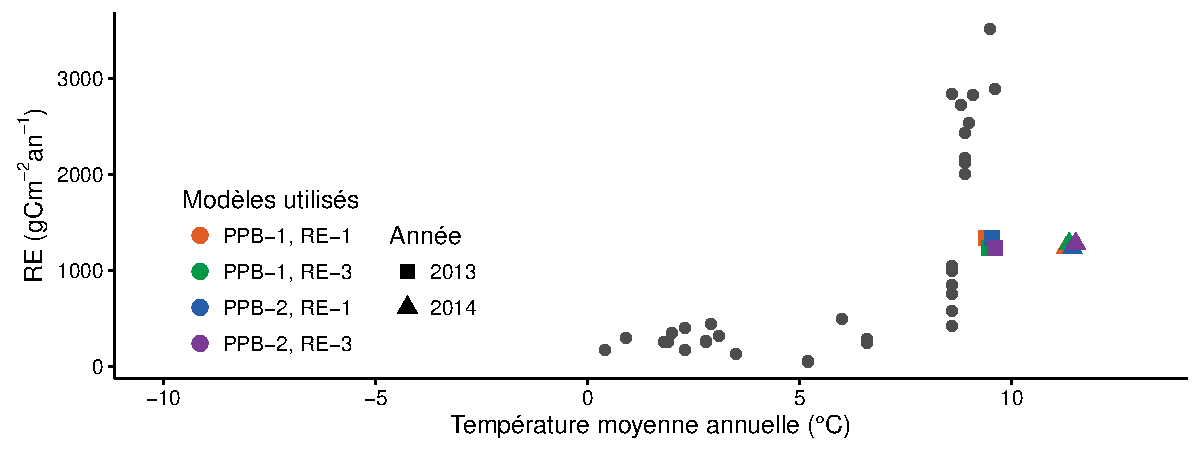
\includegraphics[width=\textwidth]{chap3/bib_vs_re}
\caption{Relation entre la respiration de l'écosystème (RE) et la température moyenne annuelle (en °C) dans la littérature (points gris) et pour ces travaux. Les couleurs correspondent aux différentes combinaisons de modèles utilisées.}
\label{fig:bib_vs_re}
\end{figure}

Les observations sur l'intensité des flux de la PPB sont également valables pour la respiration : la \textbf{RE} estimée sur la tourbière de La Guette est plus élevée que celles mesurées sur les tourbières boréales et plus faible que celles mesurées sur des prairies tourbeuses.
La RE estimée sur la tourbière de La Guette est comprise entre 1232 et \SI{1337}{\gcma} selon l'année et le modèle considéré (Figure~\ref{fig:bib_vs_re}).
Les estimations de la RE sont très proches pour les deux années, ce qui est cohérent avec le niveau de nappe d'eau relativement similaire également observé.
La différence de température de l'air entre 2013 et 2014 (\num{9.1} et \SI{10.1}{\degreeCelsius} respectivement) n'est pas suffisante pour observer une différence significative.

La comparaison de ces valeurs à celles des études citées précédemment, pour la PPB, montre qu'elles sont plus importantes que celles mesurées par \citet{peichl2014} et \citet{trudeau2014} (137 à \SI{443}{\gcma} et 206 à \SI{234}{\gcma} respectivement).
Elles s'approchent également des valeurs mesurées par \citet{beyer2015} (585 à \SI{1052}{\gcma}) et sont plus faibles que celles mesurées par \citet{jacobs2007} ou \citet{gorres2014} (500 à \SI{2000}{\gcma} et 2070 et \SI{3500}{\gcma} respectivement).
Comme pour la PPB, la température moyenne annuelle et la composition végétale des sites sont des explications possibles à ces observations.

De façon générale, les flux estimés sur la tourbière de La Guette sont cohérent avec les estimations relevées dans la littérature.

\subsubsection{Représentativité locale des flux de \coo}

Si l'on excepte la placette n°5, les modèles de la RE calibrés à l'échelle de l'écosystème permettent de représenter les placettes avec une NRMSE plus faible pour RE-3 par rapport à RE-1 : les pics des distributions sont autour de 40 et \SI{55}{\percent} respectivement (Figure~\ref{fig:repr_loc}).
Ces observations permettent de soutenir l'intérêt d'inclure l'indice de végétation dans la modélisation de la RE.

Pour la PPB (et toujours en excluant la placette n°5) la différence entre les deux modèles est moins forte (Figure~\ref{fig:repr_loc}).
La majorité des placettes ayant une NRMSE d'environ \SI{50}{\percent} pour les deux modèles.
Pour chacun d'entre eux il y a autant de placettes ayant une NRMSE inférieure à \SI{50}{\percent} (7) que de placettes ayant une NRMSE supérieure (13).
Il ne semble par y avoir de différences significatives dans la représentativité locale des modèles PPB-1 et PPB-2.

\subsubsection{\fchh}

\begin{figure}
\centering
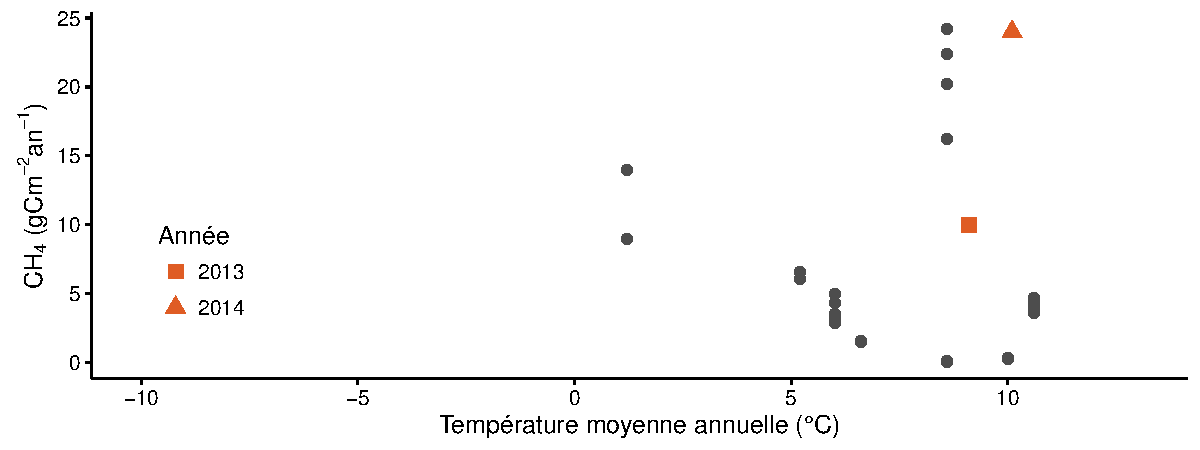
\includegraphics[width=\textwidth]{chap3/bib_vs_ch4}
\caption{Relation entre les flux de \chh  et la température moyenne annuelle (en °C) dans la littérature (points gris) et pour ces travaux (en rouge).}
\label{fig:bib_vs_ch4}
\end{figure}

Comparés aux flux de \coo, les flux de \chh mesurés sur la tourbière de La Guette sont faibles : deux ordres de grandeur inférieurs.
Ces flux sont dans la gamme des valeurs présentes dans la littérature, de 1 à \SI{40}{\gcma} (Figure~\ref{fig:bib_vs_ch4},  \citep{nilsson2001}).
Pour 2013 les valeurs mesurées sont proches de celles mesurées par \citet{nilsson2008} (entre 9 et \SI{14}{\gcma}).
L'absence d'étiage en 2014 expliquerait le doublement des flux en minimisant la zone aérobie et les possibilités d'oxydation du \chh \citep{lai2009}.
Les faibles variations du niveau de nappe sont probablement à l'origine de l'absence de relation entre ce dernier et les flux de \chh.
Ces observations corroborent les observations faites par \citet{trudeau2012} et \textbf{(à developper, de ref ds trudeau2012)}

\subsubsection{Le COD}

Les flux de COD estimés sur la tourbière de La Guette est très faible comparée aux flux de \coo.
Par ailleurs, ils sont du même ordre de grandeur que les flux de \chh.
Les quantités de COD exportées par la tourbière sont dans la gamme de celles présentes dans la littérature.
Elles sont plus faibles que celles estimées par \citet{worrall2009} (entre 10 et \SI{86}{\gcma}), mais plus importantes que celles estimées par \citet{carroll1997} dans une tourbière de bas-marais d’Amérique du nord (\SI{3.4}{\gcma}) ou celles rapportées par \citet{waddington2000} (<\SI{6}{\gcma}) dans une tourbière de haut-marais suédoise.

Le doublement du flux de COD observé en 2014 par rapport à 2013 est lié à une quantité plus importante d'eau quittant la tourbière (Figure~\ref{fig:discharge}) et présentant des concentrations en COD similaires.
Dans le même temps, le niveau de nappe moyen mesuré en 2014 est légèrement supérieur à celui mesuré en 2013 et les précipitations sont du même ordre de grandeur (Figure~\ref{fig:WTL} et \ref{fig:pluvio}).
Ces observations permettent de faire l'hypothèse que l'année 2013 a permis à la tourbière de reconstituer une partie de son stock d'eau perdu lors des années précédentes plus sèches.

\subsubsection{Incertitudes et limitations du bilan}
Les incertitudes les plus fortes du bilan sont sur les flux de \chh avec une NRMSE de \SI{32}{\percent} lors de la calibration et de \SI{68}{\percent} lors de la validation.
Cette différence importante montre que l'estimation des flux de \chh à l'aide de l'indice de végétation a permis l'estimation de sa contribution au bilan de carbone de l'écosystème pour les années 2013 et 2014, mais que son utilisation dans d'autres conditions (année sèche, température moyenne annuelle significativement différente) est limitée.
L'importance faible du \chh dans le bilan de carbone de la tourbière rend ces incertitudes moins critiques que celles faites sur l'estimation de la PPB.
Les incertitudes importantes sur la PPB, sont mises en évidence par les fortes variations des flux interpolés selon l'équation utilisée.
Elles sont la source des variations observées en termes de bilan.
À l'inverse la RE est bien contrainte.
Sur les 2 années la différence entre les différentes équations utilisées ne dépassent pas \SI{25}{\gcma}.

En outre le bilan de carbone est aussi limité par sa représentativité. 
Différents éléments n'ont pas été pris en compte dans les mesures et l'établissement du bilan.
La strate arborée notamment, largement présente dans certaines zones, n'est pas considérée directement.
Les zones, restreintes, de touradons également, de même que les arbustes dépassant la taille de la chambre ou encore les zones d'eau libre.

\subsection{Estimations du bilan net de l'écosystème à l'échelle de la tourbière de La Guette}

\begin{figure}
\centering
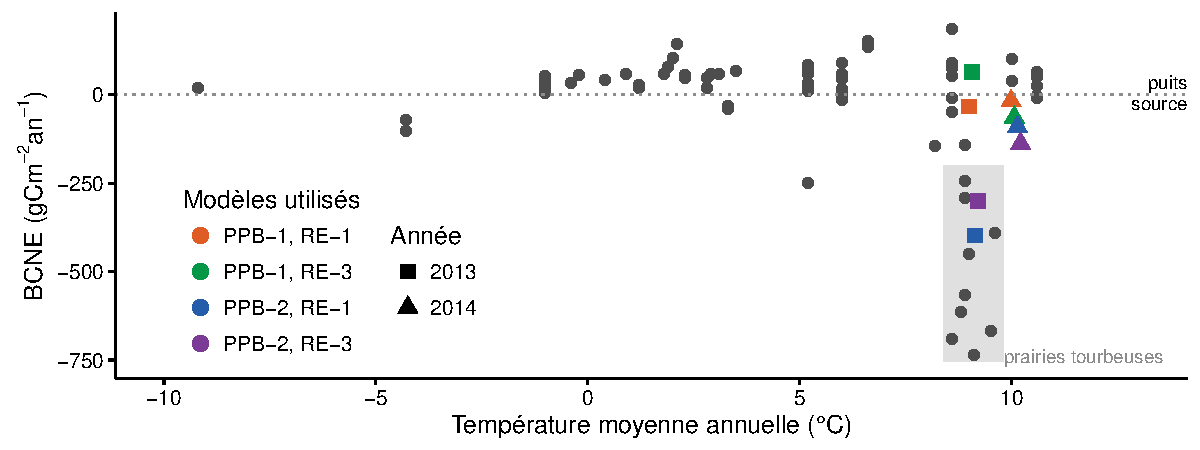
\includegraphics[width=\textwidth]{chap3/bib_vs_necb}
\caption{Relation entre le bilan de carbone net de l'écosystème (BCNE) et la température moyenne annuelle (en °C) dans la littérature (points gris) et pour ces travaux.  Les couleurs correspondent aux différentes combinaisons de modèles utilisées et la ligne de tirets sépare les écosystèmes stockant du carbone (au dessus) de ceux libérant du carbone (en dessous).}
\label{fig:bib_vs_necb}
\end{figure}

\subsubsection{Puits ou source ?}

En considérant les estimations qui semblent les plus pertinentes pour la PPB (PPB-2) et pour la RE (RE-3), on peut dire que la tourbière de La Guette est une source de carbone.
Ainsi elle émet, en moyenne sur les deux années, environ \SI{220(33)}{\gcma} (Tableau~\ref{table:bdc}).
Ces valeurs sont du même ordre de grandeur que celles mesurées dans des prairies tourbeuses (Figure~\ref{fig:bib_vs_necb}).
La tourbière est également une source de carbone plus importante en 2013 (\SI{-301(47)}{\gcma}) qu'en 2014 (\SI{-138(20)}{\gcma}).
La légère baisse du niveau de la nappe d'eau en 2013 ne se traduit pas par une RE plus importante et cette différence est principalement liée à une hausse de la PPB.
Cette hausse de la PPB est peut être liée à l'histoire du site : les années précédant les mesures sont sèches et ont pu amoindrir le potentiel de photosynthèse de l'écosystème, notamment de ses plantes pérennes (bryophytes et chaméphytes ligneux).
Ce potentiel en cours de rétablissement pendant le suivi serait donc plus fort en 2014.
Elles se rapprochent de celles mesurées dans des tourbières de bas-marais d'Amérique du nord : \SI{-145}{\gcma} \citep{carroll1997} ou celles mesurées dans une autre tourbière de bas-marais en Allemagne (\num{-142} à \SI{-565}{\gcma}) mais utilisée comme prairie permanente \citep{beyer2015}.

\subsubsection{Importance relative des flux}

D'une manière générale, les bilans sont principalement fonction de l'intensité des flux de \coo.
Le \chh et le COD ont une place marginale en termes de quantité de carbone.
Malgré tout il faut noter que le méthane a un potentiel de réchauffement global équivalent à 86 fois celui du \coo à l'horizon de 20 ans \citep{myhre2013}.
Cette caractéristique lui confère une importance élevée vis-à-vis du réchauffement malgré les faibles quantité de carbone émises.
Ces observations sont cohérentes avec d'autres études comme \citet{bortoluzzi2006a,worrall2009}.
Cependant si les quantités de C émise sous forme de \chh sont faibles dans le bilan de carbone de la tourbière de La Guette, il faut considérer le fait que seul le flux diffusif de \chh a pu être mesuré et estimé (c'est également le cas pour les études citées précédemment).
Les émissions de \chh par ébullition sont exclues du bilan.
Rarement estimé, ce flux peut représenter 17 à \SI{66}{\percent} d'une émission \citep{gogo2011,christensen2003}, et être potentiellement très fort : plus de \SI{35}{\gcm} par événement \citep{glaser2009}.
La présence de végétaux vasculaires qui en transportant le \chh dans l'atmosphère diminuent la concentration en \chh dans le sol tendraient cependant à diminuer ce phénomène \citep{chanton2005}.

\subsection{Variabilité spatiale sur la tourbière de La Guette}

\subsubsection{Distribution des groupes de végétation}

\begin{figure}
\centering
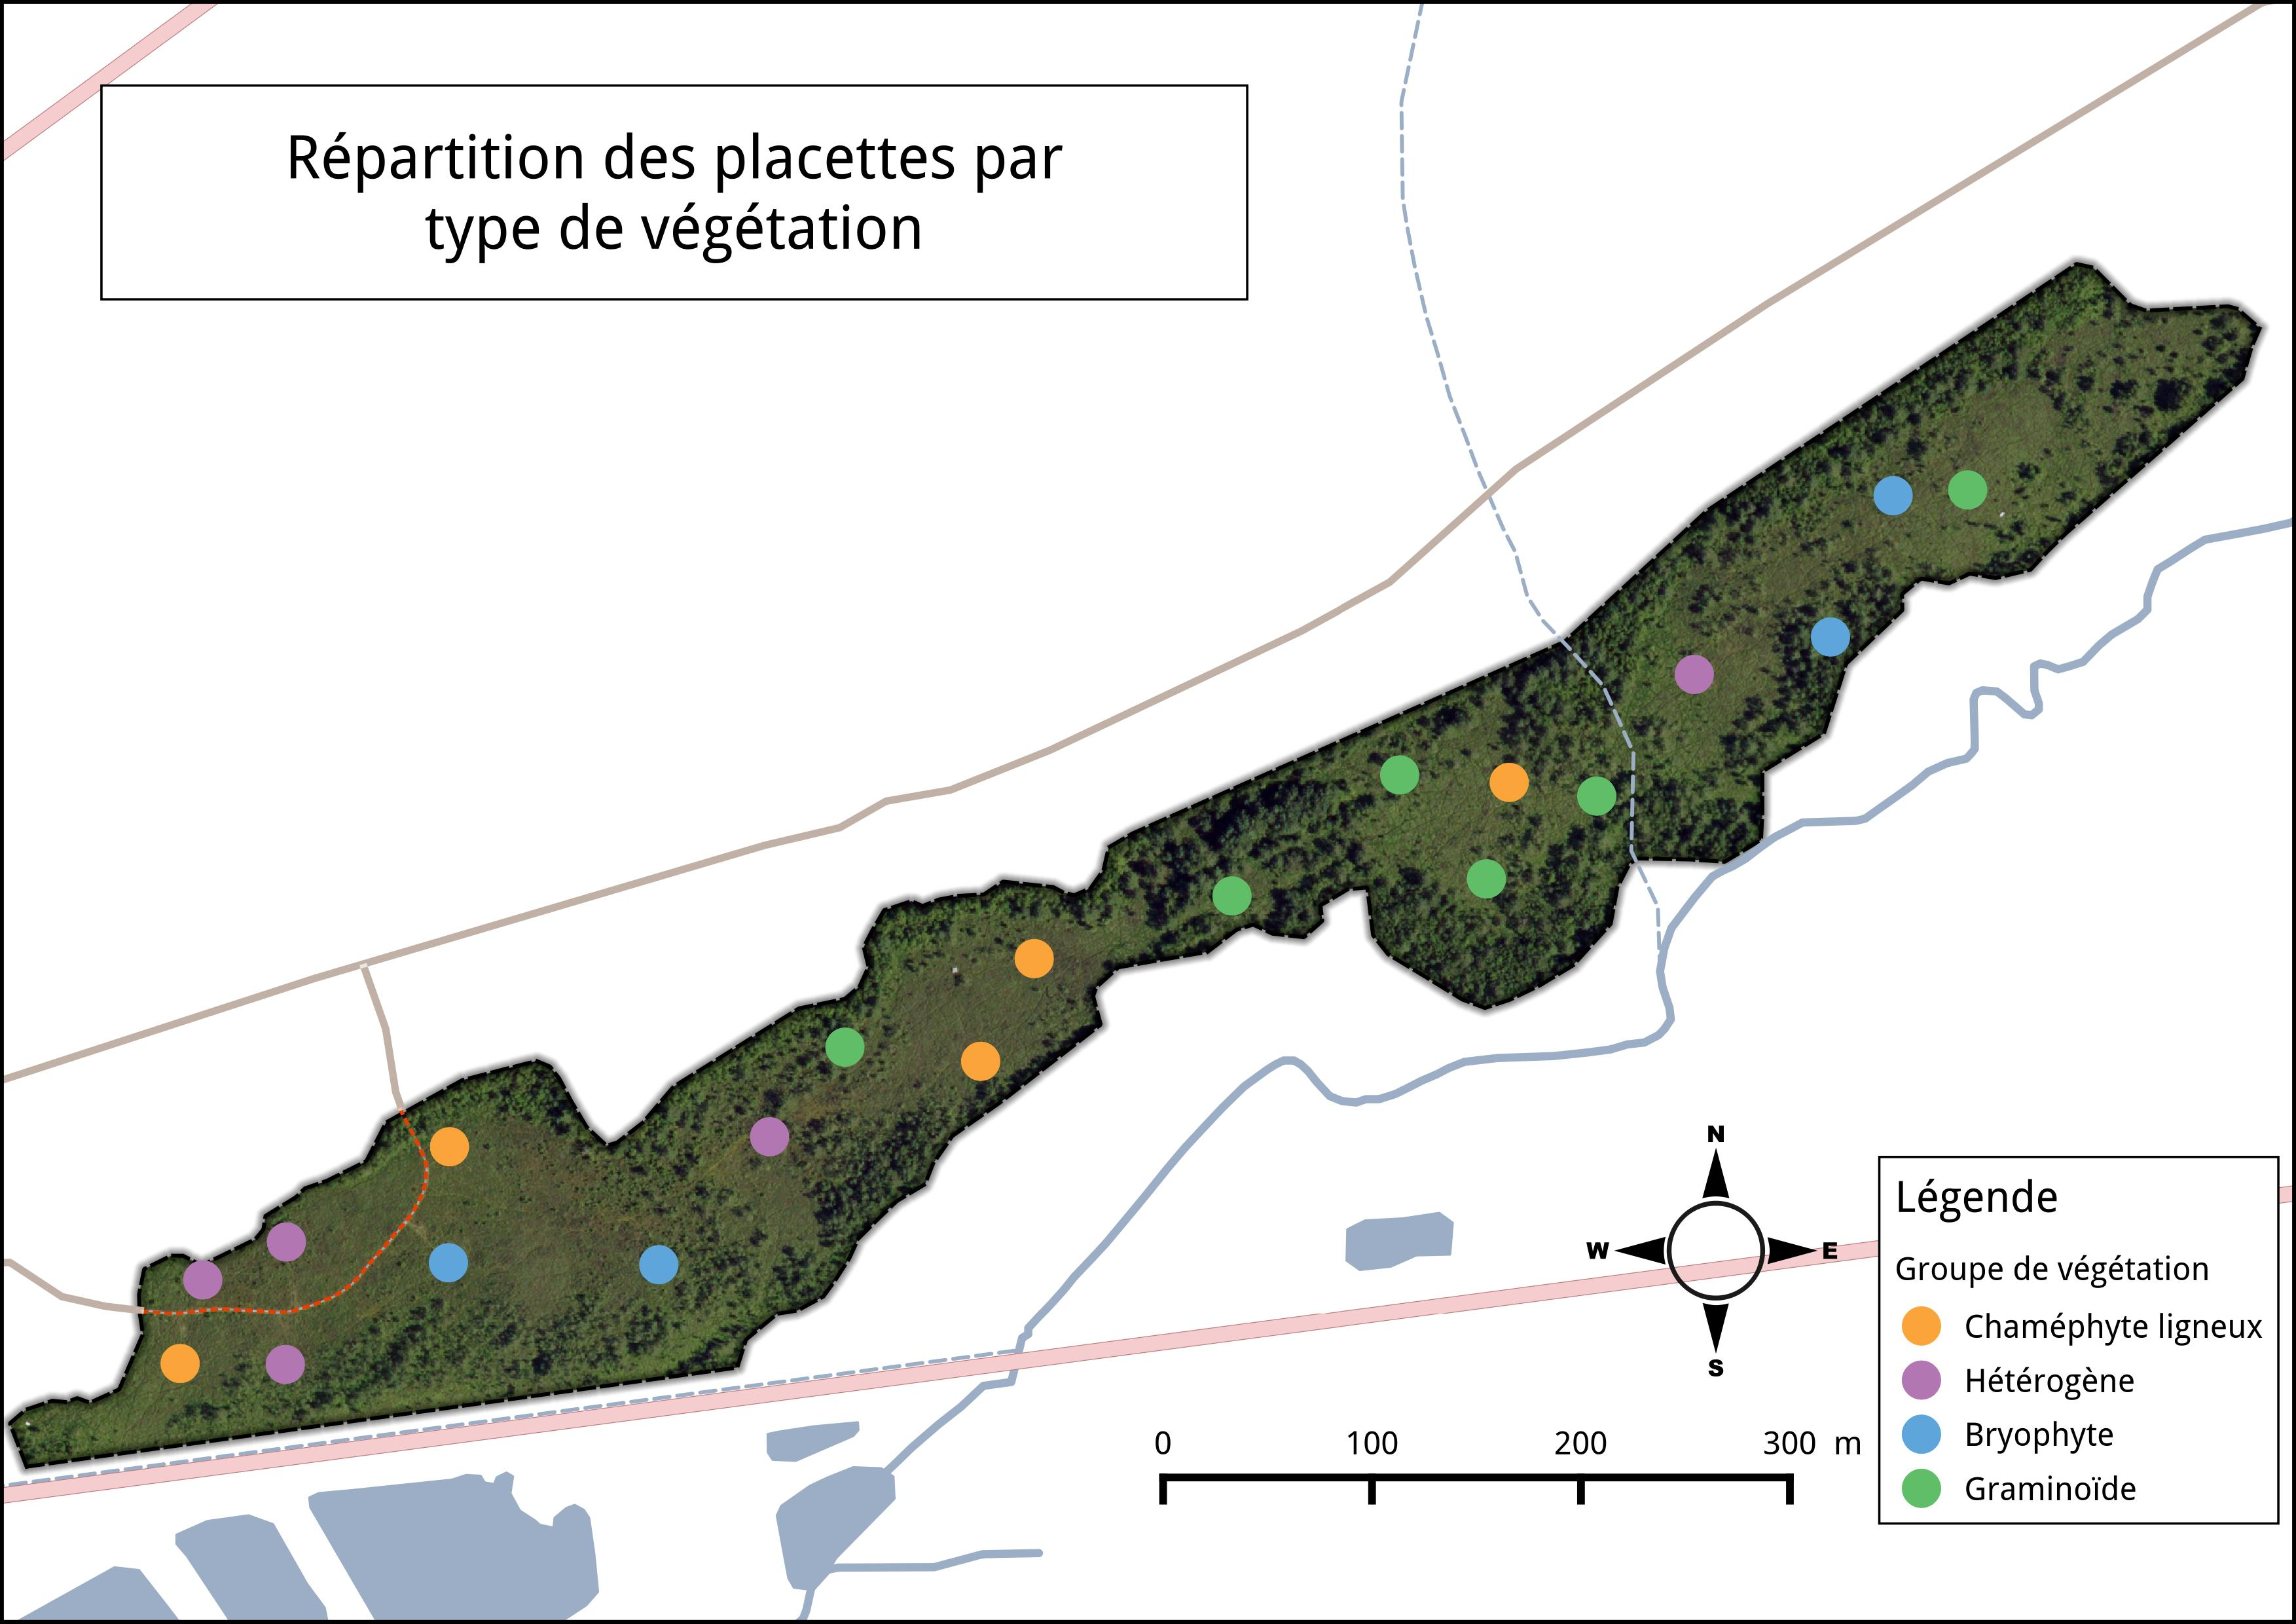
\includegraphics[width=.98\textwidth]{chap3/carte_grpveg}
\caption{Distribution des groupes de végétation sur la tourbière de La Guette.}
\label{fig:carte_grpveg}
\end{figure}

Si quelques placettes proches géographiquement ont des recouvrements végétaux voisins (les placettes p18 et p19 ; p02, p03 et p04 ; p12, p14 et p16) les autres ne présentent pas un tel lien (Figure~\ref{fig:carte_grpveg}).
Par ailleurs, au sein d'une même classe peuvent être rassemblées des placettes très éloignées spatialement, les placettes p01 et p15 par exemple ou les placettes p02 et p17 ou p09 et p20.
Ceci montre une variabilité spatiale importante du recouvrement végétal mais également que cette variabilité ne semble pas répartie géographiquement, selon un gradient quelconque.

\subsubsection{Effet du type de végétation majoritaire sur les flux et le bilan de \coo}

L'estimation des flux par groupe de végétation montre que lorsque la strate muscinale est la plus importante, l'intensité des flux est plus faible.
Cette observation est valable pour la PPB et est cohérente avec la littérature qui rapporte une productivité plus faible des sphaignes (notamment par rapport aux herbacées) \citep{rydin2013b,beyer2015}. 
La RE du groupe Bryophytes est également plus faible que celle des autres groupes.
Dans ce cas le niveau élevé de la nappe et la proportion plus faible de plantes vasculaires, qui permettent l'aération du milieu et la stimulation de la RE par la libération d'exsudats racinaires, peut expliquer la faible intensité du flux.

Les groupes Hétérogène et Chaméphyte ligneux sont proches et sont des sources de carbone importantes quelle que soit la combinaison de modèles.
La RE de ces groupes est plutôt élevée (> \SI{1200}{\gcma}), et est couplée à une PPB plutôt faible (située entre celle du groupe Bryophytes et celle du groupe Graminoïde).
Le point commun de ces deux groupes est la proportion de la strate arbustive qui dépasse \SI{50}{\percent}.
Ceci est cohérent avec la croissance limitée de la strate arbustive (par rapport à la strate herbacée) au cours de la saison de végétation (donc PPB plus faible) \citep{rydin2013b}.
La Re plus forte peut elle s'expliquer par la présence des racines.

Le groupe Graminoïde est le plus particulier, son comportement varie de façon importante en fonction des modèles.
C'est le seul groupe dont une des estimations du bilan de \coo est positive (fonction puits).
Cette observation est contraire à ce que l'on attend.
En effet notre hypothèse de départ relie un envahissement par une végétation vasculaire à une augmentation de la RE, causée par une meilleure aération du milieu, et donc à un bilan qui tendrait davantage à être une source de carbone.
Cette augmentation de la RE n'est pas visible, le groupe Graminoïde est même celui pour lequel la RE est la plus faible.
Pour expliquer cette observation on peut faire l'hypothèse que le potentiel de photosynthèse des plantes pérennes, notamment des sphaignes, n'ait pas encore retrouvé son maximum après avoir été affaibli pendant les années sèches précédant les mesures.
Cette hypothèse est cohérente avec une photosynthèse forte de la Molinie telle qu'on peut l'observer (Tableau~\ref{table:flux_grp}).
La PPB de la strate herbacée (principalement la Molinie) n'est pas ou peu limitée que ce soit par l'histoire du site.

Par ailleurs, la strate herbacée n'est pas ou peu affectée par le niveau élevé de la nappe d'eau.
En effet les espèces de cette strate (\textit{Molinia caerulea} et \textit{Eriophorum augustifolium}) ont la capacité d'échanger du gaz de leur racines à l'atmosphère grâce à l'aérenchyme, ce qui leur permet de se développer dans des milieux inondés \citep{taylor2001,rydin2013c}.
Il n'est donc pas surprenant que la Molinie se soit développée sans difficulté apparente pendant les deux années.

\subsubsection{Quantification de la variabilité spatiale}

La distribution des flux calculés par placette permet, de faire une première estimation quantifié de la variabilité spatiale.
La variabilité spatiale mesurée sur le site de La Guette est relativement importante comparée aux moyennes observées dans différents sites (Figure~\ref{fig:vs_bib}--A).
La variabilité spatiale de la RE, similaire en 2013 et 2014, l'est davantage encore (Figure~\ref{fig:vs_bib}--B).
La variabilité spatiale du bilan, dépasse les moyennes relevées dans la littérature (Figure~\ref{fig:vs_bib}--C).

Ces comparaisons sont évidemment à regarder avec précaution, l'erreur liée aux estimations faites par placette étant forte.
Néanmoins ces graphes montrent l'importance de la variabilité spatiale des flux à l'échelle d'une tourbière et permettent de mettre cette variabilité en perspective par rapport aux moyennes usuellement rapportées.

\begin{figure}[!htb]
\centering
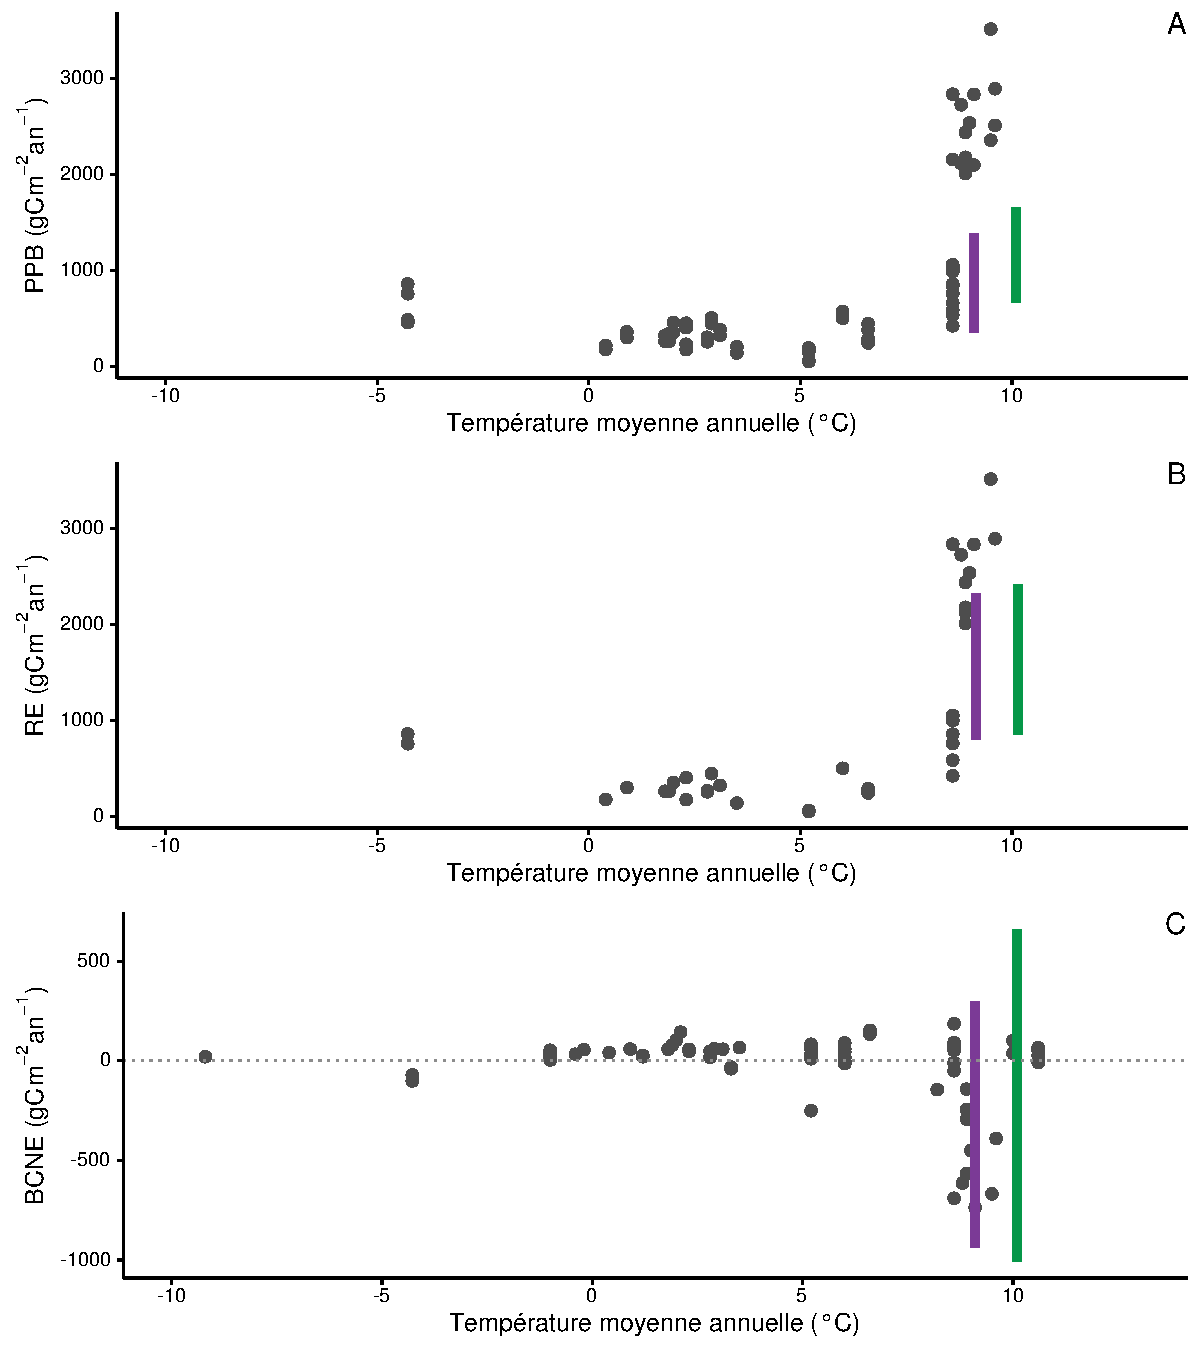
\includegraphics[width=.95\textwidth]{chap3/vs_bib}
\caption{Variabilité spatiale, par placette, des flux issus des modèles PPB-2 et RE-3, comparée aux valeurs relevées dans la littérature (points gris). Les barres violettes représentent les gammes mesurées en 2013 et les barres vertes celles mesurées en 2014. Le tableau de l'annexe~\ref{sec:bibliodata} recense les références utilisées.}
\label{fig:vs_bib}
\end{figure}

\section{Conclusions}
Le bilan de carbone établi pour la tourbière de La Guette montre qu'elle fonctionne comme une source de carbone, et qu'elle émet environ  \SI{220(33)}{\gcma} dans l'atmosphère.
Ce bilan est principalement déterminé par les flux de \coo qui sont importants, le \chh et le COD ayant des flux d'une magnitude moindre.
La calibration des modèles par groupe de placette a montré que les placette d'herbacée étaient les plus proches d'un fonctionnement en puits de carbone de par l'importance de leur photosynthèse.
Ce constat suggère l'importance de l'histoire du site et de l'effet des années précédentes, plus sèches, sur l'écosystème.
L'étude de la variabilité spatiale malgré ses limites montre l'importance qu'elle peut avoir et la nécessité de la considérer lors de l'étude de ces écosystèmes
Enfin l'importance de l'évaluation, rarement effectuée, a également été mise en avant puisqu'elle permet de mieux connaître les limites des modèles employés.
